\documentclass{book}%
\usepackage[T1]{fontenc}%
\usepackage[utf8]{inputenc}%
\usepackage{lmodern}%
\usepackage{textcomp}%
\usepackage{lastpage}%
%
\input{livre_pbs_pylatex.tex}%
\title{   \Huge \textbf{MATHÉMATIQUES EN MPSI} \\ \vspace{10pt}   \huge \textbf{ Problèmes d'automne}}%
\author{Rémy Nicolaï}%
\date{\today}%
%
\begin{document}%
\normalsize%
\maketitle \newpage \pagestyle{empty} \renewcommand{\contentsname}{Liste des problèmes} \tableofcontents \pagestyle{fancy} \addtolength{\headheight}{\baselineskip} \cfoot{\thepage} \newpage \fancyhead[LO,RE]{} \begin{center} \LARGE{\textbf{Introduction}} \end{center} %
Cet ouvrage a été publié en 2014 chez l'éditeur "In Libro Veritas". Depuis cette date, les textes qui le composent ont continués à être mis à jour. La préface de l'ouvrage publié est reproduite au dessous.



La collection "MATH\'EMATIQUES EN MPSI" propose des documents pédagogiques (recueils de problèmes corrigés, livres de cours) en complément de ceux distribués en classe.\newline
Les ouvrages de la collection sont  disponibles sur internet. En fait, ils sont \emph{produits en ligne} à partir d'une base de données (le \emph{maquis documentaire}) accessible à l'adresse
\begin{center}
 \href{http://maquisdoc.net}{http://maquisdoc.net}
\end{center}
Cette base est conçue pour être très souple. Elle accompagne les auteurs et les utilisateurs en leur permettant de travailler librement et au jour le jour.

Il est devenu impossible de travailler sans internet (y compris pour rédiger des problèmes de mathématiques) mais il est également impossible de ne travailler que sur écran. Le papier garde donc toute sa validité et la publication de livres sous la forme imprimée habituelle (à coté d'autres types de services) est encore totalement justifiée.\newline
En revanche, le modèle économique de l'édition est devenu obsolète pour de tels ouvrages péri-scolaires produits à partir de structures web. L'éditeur (\emph{In Libro Veritas}) a accepté de diffuser cette collection sous licence Creative Commons. Les auteurs peuvent ainsi user plus libéralement de leur droit d'auteur et offrir davantage de liberté aux lecteurs.

\begin{center}
 \textbf{"\emph{Problèmes d'automne}"}
\end{center}
est un recueil de problèmes corrigés.\newline
Les énoncés portent sur le "programme de début d'année" qui nous est imposé par les textes officiels. Certains textes sont de simples exercices, en particulier ceux relatifs aux calculs usuels (complexes, trigonométriques) ou aux équations différentielles. D'autres, en particulier en géométrie, sont moins immédiats. Certains sont complexes mais aucun n'est abstrait, en cela ils ne sont pas tout à fait représentatifs de ce qui demandé le reste de l'année mais forment un socle indispensable pour les problèmes de géométrie des concours.\newline
Ces textes sont indiscutablement plus difficiles que ceux du type bac et leur abord peut dérouter. L'étudiant, surtout en début d'année, ne doit pas se condamner à trouver. La lecture de la solution, après un temps de recherche assez court, s'avèrera plus rentable qu'un acharnement infructueux. Il faut aussi ne pas se contenter de trouver mais s'obliger à repérer les tournures qui cristallisent les idées, à reproduire les présentations qui valorisent la copie. Il faut rédiger !


D'autres ouvrages de la collection proposent des textes portant sur l'ensemble du programme : très simples (\emph{Problèmes basiques}) ou moins immédiats (\emph{Problèmes d'approfondissement}).
 
%
\part*{Énoncés} \addcontentsline{toc}{part}{Énoncés.} %
\section*{Problème 1}%
\addcontentsline{toc}{section}{Pb 1 : Une propriété des tangentes à la cardioïde.}%
\fancyhead[LO,RE]{Énoncés - Pb 1 : Une propriété des tangentes à la cardioïde.}%
%<dscrpt>Une propriété des tangentes à la cardioïde.</dscrpt>
Dans ce problème \footnote{d'après E3A 2006}\\ on travaille dans $\R^2$ muni d'un repère
orthonormé direct
$\mathcal{R}=(O,\overrightarrow{i},\overrightarrow{j})$. On choisit
$O$ comme pôle et $(O,\overrightarrow{i})$ comme axe polaire. On
note $\Gamma$  la courbe d'équation polaire
  $\rho=1+\cos \theta$.
  On considère l'application
  $$\fonc{\varphi}{]-\pi,\pi[}{\R}{\theta}{t=\tan\frac\theta2}.$$
\begin{figure}
	\centering
	\input{Ecardioid_1.pdf_t}
	\caption{Courbe $\Gamma$}
\end{figure}

\begin{enumerate}
  \item Montrer que :
\begin{align*}
 x &=2\frac{1-t^2}{(1+t^2)^2} \\
  y &=\frac{4t}{(1+t^2)^2}
\end{align*}
  sont des équations paramétriques de $\Gamma$ privée de l'origine.

Dans la suite du problème, on utilisera cette paramétrisation de $\Gamma$.
  \item Déterminer la direction de la tangente à $\Gamma$ au point de paramètre $t=\sqrt 3$.
  \item  Montrer que la tangente à $\Gamma$ en le point $M$ de   paramètre $\tau$ a pour équation :
\begin{displaymath}
 (\tau^3-3\tau)y+(3\tau^2-1)x+2=0
\end{displaymath}

  \item Montrer que cette tangente recoupe $\Gamma$ en deux  points  $P _1$ de paramètre $t_1$ et $P_2$ de paramètre $t_2$ (avec $t_1\neq t_2$) si et seulement si $\tau^2> 3$. Montrer que dans ce cas :
\begin{align*}
 t_1t_2=3 & & t_1+t_2=-2\tau
\end{align*}
On pourra utiliser que :
\begin{quotation}
 \`A l'aide d'un logiciel de calcul formel, en substituant $\tau +T$ à $t$ dans l'expression
\[(\tau^3-3\tau)4t+2(3\tau^2-1)(1-t^2)+2(1+t^2)\]
on obtient
\[T^4+4\tau T^3+(3\tau^2+3)T^2\]
\end{quotation}
  \item \begin{enumerate}
          \item Exprimer
\begin{displaymath}
 \begin{vmatrix}
    t_1^3-3t_1 & 3t_1^2-1 \\
    t_2^3-3t_2 & 3t_2^2-1
 \end{vmatrix}
\end{displaymath}
 en fonction de $t_1-t_2$ et $\tau$.
 \item Calculer, en fonction de $\tau$, les coordonnées du point d'intersection $N$ des tangentes aux points $P_1$ et $P_2$.
\end{enumerate}

  \item En déduire que l'ensemble des points d'intersection $N$ lorsque $\tau$ décrit 
\begin{displaymath}
 ]-\infty,-\sqrt 3 \,[ \: \cup \: ]+\sqrt 3,+\infty[
\end{displaymath}
  est inclus dans la courbe dont l'équation est :
\begin{displaymath}
 5x^2-27y^2 - 11x+2=0
\end{displaymath}
  \item Reconnaître et déterminer les éléments remarquables de cette
  courbe. La représenter dans le repère  $\cal R$.
\end{enumerate}
%
\newpage%
\section*{Problème 2}%
\addcontentsline{toc}{section}{Pb 2 : Droites, cercles : géométrie élémentaire avec des complexes. }%
\fancyhead[LO,RE]{Énoncés - Pb 2 : Droites, cercles : géométrie élémentaire avec des complexes. }%
%<dscrpt>Droites, cercles : géométrie élémentaire avec des complexes. </dscrpt>
Dans tout le problème \footnote{d'après concours général 2005}, on se place dans un plan $\mathcal P$ muni d'un repère orthonormé direct $(O,\overrightarrow{i},\overrightarrow{j})$ et on convient de désigner les points avec des capitales et les affixes avec des minuscules. Par exemple, l'affixe d'un point $M$ sera le complexe $m$, le représentant d'un nombre complexe $z$ sera le point $Z$.\newline
Soit $A$ et $B$ deux points distincts.\newline
Rappelons la définition d'une symétrie par rapport à une droite. Les points $M$ et $M'$ sont dits symétriques par rapport à la droite $(AB)$ si et seulement si:
\begin{center}
  le milieu de $M$ et $M'$ appartient à $(AB)$ et $\overrightarrow{M M'}$ est orthogonal à $\overrightarrow{AB}$.
\end{center}
\begin{figure}[!ht]
  \centering
  \includegraphics{Ecomp2_0.pdf}
  % Ecomp2_0.pdf: 142x104 px, 72dpi, 5.01x3.67 cm, bb=0 0 142 104
  \caption{Points symetriques par rapport à $(AB)$}
  \label{fig:Ecomp2_0}
\end{figure}
Rappelons aussi la définition de la médiatrice d'un segment. L'ensemble des points à égale distance de $A$ et de $B$ est une droite appelée médiatrice de $AB$.

\subsection*{Partie I. Expression complexe d'une symétrie} \noindent
Soit $A$ et $B$ deux points distincts d'affixes complexes $a$ et $b$ avec $a\neq b$.
\begin{enumerate}
  \item 
  \begin{enumerate}
    \item Donner la définition du nombre complexe $j$ et ses premières propriétés, calculer 
\[
  \frac{j^2 - j}{\overline{j^2 - j}}.
\]

    \item Soit $u$ un nombre complexe non nul. Montrer que les points d'affixes $u$, $ju$, $j^2u$ forment un triangle équilatéral.
  \end{enumerate}

  \item Soit $M$ et $M'$ (d'affixes $m$ et $m'$) deux points symétriques par rapport à $(AB)$.
  \begin{enumerate}
    \item Montrer qu'il existe $\lambda \in \R$ tel que 
    \[
      m' + m = 2a + 2(b-a)\lambda.
    \]
    \item Montrer qu'il existe $\mu \in \R$ tel que 
    \[
      m' - m = \mu i (b-a).
    \]
    \item En déduire
    \[
      \frac{m' - a}{b - a} = \overline{\left(\frac{m - a}{b-a}\right)}.
    \]
  \end{enumerate}

  \item Soit $w_1$ et $w_2$ complexes. On définit la fonction $s$ de $\C$ dans $\C$ par:
  \[
    \forall z \in \C, \; s(z) = w_1 \overline{z} + w_2.
  \]
  \begin{enumerate}
    \item En utilisant les formules de Cramer, calculer $w_1$ et $w_2$ tels que $s(a)=a$ et $s(b)=b$.
    \item Pour $z\in \C$, on note $z' = s(z)$ et $Z$, $Z'$ les points d'affixe $z$ et $z'$. Vérifier que $Z$ et $Z'$ sont symétriques par rapport à $(AB)$.
  \end{enumerate}
\end{enumerate}

\begin{figure}[!ht]
 \centering
 \includegraphics[width=5.5cm]{Ecomp2_1.pdf}
 \caption{Points $M$, $M_1$, $M_2$, $M_3$, $M_4$}
 \label{fig:Ecomp2_1}
\end{figure}

\subsection*{Partie II} \noindent
On considère les points $O$, $A$, $B$, $C$ respectivement d'affixes $0$, $1$, $j$, $j^2$.\newline
Soit $M$ un point d'affixe $m \neq 0$. On note $\rho = \vert m \vert$ et $\theta$ un argument de $m$.\newline
Soit $M_1$, $M_2$, $M_3$, $M_4$ les points symétriques de $M$ respectivement par rapport aux droites $(OA)$, $(OB)$, $(OC)$ et $(BC)$.
\begin{figure}[ht]
 \centering
 \includegraphics[width=5.5cm]{Ecomp2_2.pdf}
 \caption{Alignement de $M_2$, $M_3$, $M_4$}
 \label{fig:Ecomp2_2}
\end{figure}

\begin{enumerate}
 \item Calculer $m_1$, $m_2$, $m_3$, $m_4$ en fonction de $m$. Montrer que $M_1$, $M_2$, $M_3$ est équilatéral.
 \item Montrer que $M_2$, $M_3$, $M_4$ sont alignés si et seulement si $M$ est sur un certain cercle à préciser. Vérifier que, dans ce cas, le point $A$ est aussi sur la droite qui contient $M_2$, $M_3$, $M_4$.
 \item Si $M_2$, $M_3$, $M_4$ ne sont pas alignés, il existe un cercle (appelé cercle circonscrit) qui contient ces trois points.  On note $\Omega$ (d'affixe $\omega$) le centre de ce cercle et $R$ son rayon. On pourra utiliser que le point $\Omega$ est l'intersection des médiatrices des segments $M_2 M_3$, $M_2 M_4$, $M_3 M_4$.
    \begin{enumerate}
     \item Montrer que $O$ et $M_1$ appartiennent à la médiatrice de $M_2 M_3$. En déduire qu'il existe $\lambda$ réel tel que $\omega = \lambda e^{-i \theta}$.
     \item En utilisant le fait que $\Omega$ appartient à la médiatrice de $M_2 M_3$, montrer que
 \[
 \omega = - \frac{1+2\rho \cos \theta}{\rho +2 \cos \theta} \, e^{-i \theta}.
 \]
     \item Montrer que 
\[
  R^2= \rho^2 +\frac{(1-\rho^2)(1+2\rho \cos \theta)}{(\rho + 2 \cos \theta)^2}.
\]
    \end{enumerate}

\item Préciser géométriquement l'ensemble $\Gamma$ des points $M$ tels que les cercles circonscrits à $M_1$, $M_2$, $M_3$ et à $M_2$, $M_3$, $M_4$ aient les mêmes rayons.\newline
Reproduire approximativement, compléter et interpréter les figures~\ref{fig:Ecomp2_3} et \ref{fig:Ecomp2_4} des configurations 1 et 2.
\end{enumerate}

\begin{figure}[ht]
 \centering
 \includegraphics[width=4cm]{Ecomp2_3.pdf}
 \caption{Configuration 1}  \label{fig:Ecomp2_3}
\end{figure}
\begin{figure}[ht]
 \centering
 \includegraphics[width=4cm]{Ecomp2_4.pdf}
  \caption{Configuration 2}\label{fig:Ecomp2_4}
\end{figure}

\clearpage

%
\newpage%
\section*{Problème 3}%
\addcontentsline{toc}{section}{Pb 3 : Propriété des nombres complexes. Etude d'une famille d'équations }%
\fancyhead[LO,RE]{Énoncés - Pb 3 : Propriété des nombres complexes. Etude d'une famille d'équations }%
%<dscrpt>Propriété des nombres complexes. Etude d'une famille d'équations </dscrpt>
Dans tout l'exercice, $n$ désigne un entier naturel non nul, $\mathcal P _n$ désigne l'ensemble des entiers pairs entre $0$ et $n$ et $\mathcal I _n$ désigne l'ensemble des entiers impairs entre $0$ et $n$.

On associe à chaque paramètre complexe $a\neq 0$ deux équations d'inconnue $z$ notées $E_0(n,a)$ et $E_1(n,a)$
\begin{eqnarray*}
 E_0(n,a):\quad \quad \sum_{k\in \mathcal P _n} \binom{n}{k} z^k a^{n-k}&=& 0  \\
 E_1(n,a):\quad \quad \sum_{k\in \mathcal I _n} \binom{n}{k} z^k a^{n-k}&=& 0
\end{eqnarray*}

\begin{enumerate}
 \item Cas particuliers. Former les six équations obtenues pour $n=2$, $n=3$, $n=4$. Dans chaque cas, donner l'ensemble des solutions.
 \item Soit $\lambda$ un nombre complexe non nul, montrer que $w$ est solution de $E_0(n,a)$ si et seulement si $\lambda w$ est solution de $E_0(n,\lambda a)$
 \item 
  \begin{enumerate}
    \item Discuter selon le paramètre complexe $w$ et donner l'ensemble des solutions de l'équation d'inconnue $z$
\begin{displaymath}
 \frac{a+z}{a-z} = w
\end{displaymath}
     \item Pour $\alpha$ réel et $w=e^{i\alpha}$, simplifier
\begin{displaymath}
 \frac{w-1}{w+1}
\end{displaymath}
     \item Déterminer l'ensemble des solutions de l'équation d'inconnue $z$
\begin{displaymath}
 \left( \frac{a+z}{a-z}\right) ^n =1
\end{displaymath}
On exprimera chaque solution sous une forme simple.
     \item En considérant $(z+a)^n$ et $(-z+a)^n$ résoudre l'équation $E_1(n,a)$.
  \end{enumerate}
\item Une autre idée.
\begin{enumerate}
 \item Soit $x$ et $y$ deux nombres réels, exprimer avec des sommations les parties réelle et imaginaire de $(x+iy)^n$.
 \item Montrer que lorsque $\theta$ est un réel tel que $\cos \theta \neq 0$ :
\begin{displaymath}
 \frac{\cos(n\theta)}{\cos ^n \theta} = \sum_{k\in \mathcal P _n} \binom{n}{k} (i \tan \theta )^{k}, \hspace{0.5cm}
 i\,\frac{\sin(n\theta)}{\cos ^n \theta} = \sum_{k\in \mathcal I _n} \binom{n}{k} (i\tan \theta)^k
\end{displaymath}
\item En déduire les solutions de $E_1(n,1)$ puis retrouver celles de $E_1(n,a)$ déjà obtenues en 3.d.
 \item Déterminer les solutions de $E_0(n,i)$ puis de $E_0(n,a)$.
\end{enumerate}

\end{enumerate}


%
\newpage%
\section*{Problème 4}%
\addcontentsline{toc}{section}{Pb 4 : Ellipse: ``bande de papier'' et cercles de Chasles.}%
\fancyhead[LO,RE]{Énoncés - Pb 4 : Ellipse: ``bande de papier'' et cercles de Chasles.}%
%<dscrpt>Ellipse: `bande de papier` et cercles de Chasles.</dscrpt>
\begin{figure}
	\begin{center}
	\input{Econi1_1.pdf_t}
	\end{center}
\caption{Bande de papier.}
\end{figure} 
Sur une bande de papier, on place trois points $Q$, $M$, $P$. Le point $M$ est entre $P$ et $Q$ avec $QM=a\geq MP=b>0$ comme sur la figure.\newline
Un repère orthonormé $(O,\overrightarrow{i},\overrightarrow{j})$ étant fixé, on fait glisser la bande de papier en plaçant le point $Q$ sur l'axe $(Oy)$ et le point $P$ sur l'axe $(Ox)$. On note $\mathcal E$ l'ensemble décrit par les points $M$.
\begin{enumerate}
    \item Construire quelques points de $\mathcal E$ sur une figure.
    \item On note $I$ le point du plan dont les projetés orthogonaux sur les axes sont $P$ et $Q$. On note  $\theta$ l'angle orienté $(\overrightarrow{i},\overrightarrow{OI})$.
    \begin{enumerate}
       \item Calculer $\Vert \overrightarrow{OI} \Vert$.
       \item  Calculer en fonction de $\theta$ les coordonnées de $P$, $Q$, $M$.
       \item Que peut-on en déduire pour $\mathcal E$ ?
    \end{enumerate}

\item (cercles de Chasles) On définit les points $I_\theta$ et $J_\theta$ par :
\begin{align*}
 \overrightarrow{OI_\theta}=(a+b)\overrightarrow{e}_\theta & &
 \overrightarrow{OJ_\theta}=(a-b)\overrightarrow{e}_{-\theta}
\end{align*}
Montrer que le milieu de $[I_\theta, J_\theta]$ est le point $M$ et que la droite $(I_\theta, J_\theta)$ est la normale en $M$ à $\mathcal E$. 
\end{enumerate}
%
\newpage%
\section*{Problème 5}%
\addcontentsline{toc}{section}{Pb 5 : Coniques, enveloppes, cercles directeurs.}%
\fancyhead[LO,RE]{Énoncés - Pb 5 : Coniques, enveloppes, cercles directeurs.}%
%<dscrpt>Coniques, enveloppes, cercles directeurs.</dscrpt>
Dans ce problème, la partie V est indépendante des autres.

Un plan est rapporté à un repère $\mathcal R = (A,\overrightarrow{i},\overrightarrow{j})$. On note
\begin{displaymath}
 \overrightarrow{e}_\theta = \cos \theta \overrightarrow{i}+ \sin \theta \overrightarrow{j}
\end{displaymath}
Soit $a$ et $c$ deux réels strictement positifs. On introduit, pour $\theta \in ]-\pi,\pi]$,  les éléments suivants:
\begin{itemize}
 \item le point $B$ de coordonnées $(2c,0)$
\item le point $C_\theta$  défini par :
\begin{displaymath}
 \overrightarrow{AC_\theta} = 2a \overrightarrow{e}_\theta 
\end{displaymath}
\item la médiatrice $\mathcal{D}_\theta$  de $[B,C_\theta]$.
\item le milieu $H_\theta$ de $[B,C_\theta]$.
\item le point d'intersection $M_\theta$ (lorsqu'il existe) des droites $\mathcal{D}_\theta$ et $(AC_\theta)$.
\item l'ensemble $\mathcal C$ des points $M_\theta$.
\item le nombre $\theta_0 = \arccos \frac{a}{c}$ lorsque $a<c$.
\end{itemize}
Ces notations sont valables dans tout le problème.
\subsubsection*{Partie I. Situation géométrique. Calculs complexes.}
Lorsque $M$ est un point quelconque du plan, on note $z(M)$ l'affixe de $M$ relative au repère $\mathcal R$.
\begin{enumerate}
 \item Faire une figure dans chacun des trois cas :
\begin{align*}
 0<c<a &,& 0<c=a &,& 0<a<c
\end{align*}
\item Quel est l'ensemble $\mathcal C$ lorsque $c=a$ ? Dans toute la suite du problème, on supposera $c\neq a$.
\item Calculer les affixes de $A$, $B$, $C_\theta$, $H_\theta$. Quel est l'ensemble des $H_\theta$ lorsqe $\theta$ décrit $]-\pi,\pi]$ ?
\item 
\begin{enumerate}
 \item Justifier l'existence d'un $\lambda \in \R$ tel que $z(M_\theta)=\lambda e^{i\theta}$.
 \item Montrer que
\begin{displaymath}
 (\lambda-a-ce^{-i\theta})(a-ce^{i\theta}) \in i \R
\end{displaymath}
\item Préciser les $\theta$ pour lesquels $M_\theta$ existe et calculer $z(M_\theta)$.
\end{enumerate}
\item Dans les cas $c<a$ puis $a<c$, former le tableau des signes de
\begin{displaymath}
 \frac{a^2-c^2}{a-c\cos \theta}
\end{displaymath}
pour $\theta \in ]-\pi,\pi]$
\end{enumerate}
\subsubsection*{Partie II. Définition bifocale.}
\begin{enumerate}
 \item Montrer que
\begin{displaymath}
 \left \Vert \overrightarrow{M_\theta C_\theta}\right\Vert = \left \Vert \overrightarrow{M_\theta B}\right\Vert 
\end{displaymath}
\item En discutant de la position relative des trois points alignés $A$, $M_\theta$ et $C_\theta$, montrer que $\mathcal C$ est une conique de foyers $A$ et $B$. On fera une figure dans chaque cas.
\end{enumerate}
\subsubsection*{Partie III. Enveloppes.}
Dans cette partie, $I$ est un intervalle de $\R$ et $U$,$V$,$W$ sont trois fonctions dérivables définies dans $I$ (à valeurs dans $\R$) telles que, pour tous les $t$ de $I$:
\begin{align*}
 U(t)V^\prime (t) - U^\prime (t)V(t)\neq 0 &,& (U^\prime (t),V^\prime(t))\neq (0,0)
\end{align*}
 On définit les droites $\Delta_t$ et $\Delta^\prime _t$ par leurs équations :
\begin{align*}
 \Delta_t &:& U(t)x+V(t)y+W(t)=0 \\
\Delta^\prime_t &:& U^\prime(t)x+V^\prime(t)y+W^\prime(t)=0 
\end{align*}
\begin{enumerate}
 \item Montrer que les droites $\Delta_t$ et $\Delta^\prime_t$ se coupent. On note $f(t)$ leur point d'intersection. La courbe paramétrée $f$ est appelée \emph{enveloppe} de la famille de droites. Le support de la courbe paramétrée $f$ est noté $\mathcal F$.
\item Montrer que $\Delta_t$ est tangente en $f(t)$ à $\mathcal F$.
\item Exemple. Soit $\mathcal C_1$ un cercle de centre $O$ (coordonnées $(0,0)$) et de rayon $R$ et $S$ un point de coordonnées $(s,0)$. On supposera $0<s<R$.
\begin{enumerate}
\item Soit $M$ un point de coordonnées $(R\cos t, R\sin t)$, former l'équation cartésienne de la droite (notée $\Delta_t$) perpendiculaire à $(SM)$ et passant par $M$.
\item Former la courbe paramétrée $f$ enveloppe de ces droites comme en 1.
\end{enumerate}
\end{enumerate}
\subsubsection*{Partie IV. Médiatrices.}
\begin{enumerate}
 \item Former l'équation de $\mathcal D _\theta$.
\item On note $\mathcal{D}^\prime _\theta$ l'équation obtenue à partie de $\mathcal D _\theta$ en dérivant chaque coefficient (comme en III). Montrer que $\mathcal D _\theta$ et $\mathcal D ^\prime _\theta$ se coupent en $M_\theta$. En déduire que $\mathcal D _\theta$ est tangente en $M_\theta$ à $\mathcal C$.
\item Calculer le produit des distances
\begin{displaymath}
 d(A,\mathcal D _\theta)d(B,\mathcal D _\theta)
\end{displaymath}
 des points $A$ et $B$ à la droite $\mathcal D _\theta$.
\item Quelle est la courbe formée par la projection d'un foyer sur les tangentes à une hyperbole ou une ellipse ? (Une telle courbe est appelée podaire)
\end{enumerate}
\subsubsection*{Partie V. Podaire d'un foyer sur une parabole.}
Soit $\mathcal P$ une parabole de foyer $F$ et de directrice $\mathcal D$. On choisit un repère dans lequel :
\begin{itemize}
 \item l'équation de $\mathcal D$ est
\begin{displaymath}
 x+\frac{p}{2}=0
\end{displaymath}
\item les coordonnées de $F$ sont $(\frac{p}{2},0)$
\end{itemize}
\begin{enumerate}
 \item \begin{enumerate}
 \item Former l'équation cartésienne de $\mathcal P$.
 \item Montrer que $\mathcal P$ est le support de la courbe paramétrée $u \rightarrow M_u$ définie dans $\R$ où $M_u$ est le point de coordonnées $(2pu^2,2pu)$.
\end{enumerate}
\item \'Ecrire une équation cartésienne de la tangente $\mathcal T_u$ en $M_u$ à $\mathcal P$.

On note dans toute la suite $K_u$ le projeté orthogonal de $M_u$ sur $\mathcal D$.

\item Calculer la distance de $F$ à $\mathcal T_u$, calculer la distance de $K_u$ à $\mathcal T_u$. Que peut-on en déduire ?
\item  Quel est l'ensemble des projetés orthogonaux de $F$ sur les tangentes à la parabole ?
\end{enumerate}

%
\newpage%
\section*{Problème 6}%
\addcontentsline{toc}{section}{Pb 6 : Strophoïde et cissoïde}%
\fancyhead[LO,RE]{Énoncés - Pb 6 : Strophoïde et cissoïde}%
%<dscrpt>Strophoïde et cissoïde.</dscrpt>
L'objet du probl{\`e}me\footnote{d'après Ecole de l'Air MP 2002} est
la recherche de lieux g{\'e}om{\'e}triques conduisant {\`a}
l'{\'e}tude de courbes planes (appel{\'e}es en g{\'e}n{\'e}ral
cubiques circulaires). Les parties I et II donnent deux exemples de
telles courbes. Dans la troisi{\`e}me partie, on consid{\`e}re le
cas g{\'e}n{\'e}ral.

Dans toute la suite, le plan est rapport{\'e} {\`a} un rep{\`e}re
orthonorm{\'e} d'origine not{\'e}e $O$, d'axes $Ox$ et $Oy$ et on
d{\'e}signe par $a$ un nombre r{\'e}el strictement positif
donn{\'e}.

\subsection*{PARTIE I. \'Etude de la stropho{\"i}de droite}
\begin{figure}[ht]
 \centering
  \input{Ecubcirc_1.pdf_t}
\caption{Définition de la strophoïde droite}
\end{figure}

On d{\'e}signe par $D$ la droite d'{\'e}quation $x = 2a$ et par $C$
le cercle de centre $M_{0}$ de coordonnées $(-2a, 0)$, de rayon $2a$.\newline
Pour tout nombre r{\'e}el $\theta$, on d{\'e}signera par :
\begin{itemize}
\item $H(\theta)$ le point d'intersection, lorsqu'il existe, de la droite (notée $D_\theta$) d'angle polaire $\theta$ et de la droite $D$.
\item $M(\theta)$ le point d'intersection de la droite d'angle polaire $\theta$ et du cercle $C$ (avec la convention que lorsqu'il y a deux points d'intersection, $M(\theta)$ d{\'e}signe le point d'intersection distinct de $O$).
\end{itemize}

\begin{enumerate}
\item Donner une {\'e}quation cart{\'e}sienne, puis une {\'e}quation polaire du cercle $C$.
\item D{\'e}terminer des coordonn{\'e}es polaires de $M(\theta)$ et $H(\theta)$, puis du milieu $I(\theta)$ du segment $[M(\theta)H(\theta)]$.\newline
En d{\'e}duire, lorsque $\theta$ varie, que $I(\theta)$ d{\'e}crit la courbe d'{\'e}quation polaire :
$$r(\theta) = -a \dfrac{\cos{(2\theta)}}{\cos{(\theta)}}.$$

\item Exprimer $r(\theta + 2\pi)$, $r(\pi + \theta)$, $r(-\theta)$  en fonction de $r(\theta)$. Interpr{\'e}ter g{\'e}om{\'e}triquement ces r{\'e}sultats et indiquer sur quelle partie $E$ de $\R$ il suffit d'{\'e}tudier la courbe.

\item D{\'e}terminer la limite de $r(\theta) \sin{(\theta - \pi/2)}$ lorsque $\theta$ tend vers $\pi/2$. Qu'en d{\'e}duit-on g{\'e}om{\'e}triquement ?

\item \'Etudier le signe de $r(\theta)$ pour $\theta \in E$, repr{\'e}senter sur une m{\^e}me figure la droite $D$, le cercle $C$, et
le support de cette courbe $\theta \mapsto I(\theta)$.


\item Donner enfin une {\'e}quation cart{\'e}sienne du support de la courbe $\theta \mapsto I(\theta)$.
\end{enumerate}

\subsection*{PARTIE II. \'Etude de la cisso{\"i}de droite}
\begin{figure}[ht]
 \centering
  \input{Ecubcirc_2.pdf_t}
\caption{Définition de la cissoïde droite}
\end{figure}

\medskip
On d{\'e}signe par $D$ la droite d'{\'e}quation $x = 2a$ et par $C$
le cercle de centre $M_{0} (-a, 0)$, de rayon $a$.\newline
Pour tout nombre r{\'e}el $t$, on d{\'e}signera par :
\begin{itemize}
\item $H(t)$ le point d'intersection de la droite (notée $D_t$) d'{\'e}quation $y = tx$ et de la droite $D$.
\item $M(t)$ le point d'intersection de la droite d'{\'e}quation $y = tx$ et du cercle $C$ (avec la convention que lorsqu'il y a deux points d'intersection, $M(t)$ d{\'e}signe le point d'intersection distinct de $O$).
\end{itemize}
\begin{enumerate}
\item Donner une {\'e}quation cart{\'e}sienne du cercle $C$.
\item D{\'e}terminer les coordonn{\'e}es de $M(t)$ et $H(t)$, puis du milieu $J(t)$ du segment $[M(t)H(t)]$.
\item D{\'e}terminer le vecteur-d{\'e}riv{\'e} {\`a} la courbe $t \mapsto J(t)$, puis en d{\'e}duire le(s) point(s) stationnaire(s)
 (c'est-{\`a}-dire non r{\'e}gulier(s)) de celle-ci. Etudier la tangente au(x) point(s) stationnaire(s).

En d{\'e}duire que la tangente {\`a} la courbe $t \mapsto J(t)$ au
point $J(t_{0})$ a pour {\'e}quation 
$$ t_{0} (t_{0}^{2} + 3)x - 2y = a t_{0}^{3} $$

\item Etudier les variations des coordonn{\'e}es $x(t)$, $y(t)$ du point $J(t)$ pour $t \in \R_{+}$, et repr{\'e}senter sur une m{\^e}me figure la droite $D$, le cercle $C$, et le support de cette courbe $t \mapsto J(t)$.

\item Donner enfin une {\'e}quation cart{\'e}sienne du support de la courbe $t \mapsto J(t)$.
\end{enumerate}



\subsection*{PARTIE III. \'Etude g{\'e}n{\'e}rale des cubiques
circulaires}

On consid{\`e}re un point $M_{0} (x_{0}, y_{0})$ distinct de $O$ et
on d{\'e}signe alors par $D$ la droite d'{\'e}quation $x = 2a$ et
par $C (x_{0}, y_{0})$ le cercle de centre $M_{0} (x_{0}, y_{0})$
passant par $O$.\newline
Pour tout nombre r{\'e}el $t$, on d{\'e}signera par :
\begin{itemize}
\item $H(t)$ le point d'intersection de la droite (notée $D_t$) d'{\'e}quation $y = tx$ et de la droite $D$.
\item $M(t)$ le point d'intersection de la droite d'{\'e}quation $y = tx$ et du cercle $C (x_{0}, y_{0})$ (avec la convention que lorsqu'il y a deux points d'intersection, $M(t)$ d{\'e}signe le point d'intersection distinct de $O$).
\end{itemize}
\begin{enumerate}
\item D{\'e}terminer les coordonn{\'e}es de $M(t)$ et $H(t)$, puis du milieu $K(t)$ du segment $[M(t)H(t)]$.
\item \'Etudier les branches infinies de la courbe $t \mapsto K(t)$.
\item \`A quelle condition sur $M_{0} (x_{0}, y_{0})$ l'origine $O$ appartient-elle au support de la courbe paramétrée $t \mapsto K(t)$ ?\newline
Repr{\'e}senter graphiquement la zone du plan correspondante.

\item \`A quelle condition sur $M_{0} (x_{0}, y_{0})$ la courbe a-t-elle un point double ? \newline
Quel est alors ce point double ? Repr{\'e}senter graphiquement la
zone du plan correspondante.

\item \`A quelle condition sur $M_{0} (x_{0}, y_{0})$ la courbe a-t-elle un point stationnaire (c'est {\`a} dire non r{\'e}gulier) ?\newline
Quel est alors ce point stationnaire ? Repr{\'e}senter graphiquement la zone du plan correspondante.
\end{enumerate}
%
\newpage%
\section*{Problème 7}%
\addcontentsline{toc}{section}{Pb 7 : Sommes de nombres complexes. Noyaux de Dirichlet et de Fejer.}%
\fancyhead[LO,RE]{Énoncés - Pb 7 : Sommes de nombres complexes. Noyaux de Dirichlet et de Fejer.}%
%<dscrpt>Sommes de nombres complexes. Noyaux de Dirichlet et de Fejer.</dscrpt>
Pour $n$ entier naturel sup{\'e}rieur ou {\'e}gal 1 et $\theta$ r{\'e}el, on
pose \footnote{D'apr{\'e}s CCMP 2001 2 eme {\'e}preuve}
\begin{displaymath}
  D_n(\theta)=\sum_{k=-n+1}^{n-1}e^{ik\theta} \hspace{1.5cm}
  F_n(\theta)=\frac{1}{n}\sum_{j=1}^n D_j(\theta) 
\end{displaymath}
\begin{enumerate}
  \item Sans chercher à calculer $D_n$, montrer que
\begin{displaymath}
F_n(\theta)=\sum_{k=-n+1}^{n-1}(1-\frac{|k|}{n})e^{ik\theta}  
\end{displaymath}
  \item Pour $\theta \not \in 2\pi\Z$, en calculant $D_n(\theta)$ à l'aide d'une somme de termes en progresssion géométrique, exprimer $nF_n(\theta)$ comme le carr{\'e} d'un quotient de sinus. (ne pas chercher à utiliser la première question)
\end{enumerate}
%
\newpage%
\section*{Problème 8}%
\addcontentsline{toc}{section}{Pb 8 : Des exercices sur des calculs dans R et des fonctions usuelles.}%
\fancyhead[LO,RE]{Énoncés - Pb 8 : Des exercices sur des calculs dans R et des fonctions usuelles.}%
%<dscrpt>Des exercices sur des calculs dans R et des fonctions usuelles.</dscrpt>
\begin{enumerate}
\item  R{\'e}soudre
\[
\left( \frac{z+i}{z-i}\right) ^{3}+\left( \frac{z+i}{z-i}\right) ^{2}+\left(
\frac{z+i}{z-i}\right) +1=0
\]

\item  Si $a_{0},a_{1},\cdots ,a_{n}$ sont des nombres complexes et
\[
P(z)=a_{0}+a_{1}z+\cdots +a_{n}z^{n}
\]
comment s'exprime $P(z)-P(-z)$ ?\newline
R{\'e}soudre
\[
z^{7}+\binom{7}{2}z^{5}+\binom{7}{4}z^{3}+\binom{7}{6}z=0
\]

\item  D{\'e}terminer l'ensemble des r{\'e}els $x$ tels que
\[
\sin x+\sin 2x<\sin 3x
\]

\item  Montrer que
\[
\arctan 1+\arctan 2+\arctan 3=\pi
\]


\item  Pr{\'e}senter dans un tableau les valeurs de $\arccos (\left| \cos
x\right| )$ et $\arcsin (\left| \sin x\right| )$ dans les intervalles $%
\left[ 0,\frac{\pi }{2}\right] $, $\left[ \frac{\pi }{2},\pi \right] $, $%
\left[ \pi ,\frac{3\pi }{2}\right] $, $\left[ \frac{3\pi }{2},2\pi \right] $

\end{enumerate}
%
\newpage%
\section*{Problème 9}%
\addcontentsline{toc}{section}{Pb 9 : Sommations et nombres complexes.}%
\fancyhead[LO,RE]{Énoncés - Pb 9 : Sommations et nombres complexes.}%
%<dscrpt>Sommations et nombres complexes.</dscrpt>
\begin{enumerate}
\item D{\'e}montrer que 
 \begin{displaymath}
\binom{n}{1}\frac{1}{1}- \binom{n}{2}\frac{1}{2}+\cdots+(-1)^{n-1} \binom{n}{n}\frac{1}{n}=1+\frac{1}{2}+\frac{1}{3}+\cdots+\frac{1}{n} 
 \end{displaymath}

\item Soit $n$ un entier naturel non nul, calculer $\sum_{(i,j)\in T}ij$ avec 
\begin{displaymath}
 T=\left\{ (i,j)\in \left\{ 1,\ldots ,n\right\} ^{2} \  \mathrm{ tq } \ i\leq j\right\}
\end{displaymath}

\item Soit $n$ un entier naturel non nul, calculer $R_{n}^{2}+I_{n}^{2}$ avec
\begin{align*}
 R_{n}=\sum_{k=0}^{\lfloor \frac{n}{2}\rfloor} (-1)^{k}\binom{n}{2k} & & I_{n}=\sum_{k=0}^{\lfloor \frac{n-1}{2}\rfloor} (-1)^{k}\binom{n}{2k+1}
\end{align*}

\item Soit $n$ un entier naturel non nul, $a_{1},a_{2},\cdots ,a_{n}$ des r{\'e}els strictement positifs, montrer
\begin{displaymath}
(a_{1}+a_{2}+\cdots +a_{n})(\frac{1}{a_{1}}+\frac{1}{a_{2}}+\cdots +\frac{1}{a_{n}}) \geq n^{2} 
\end{displaymath}

\item Soit $n$ un entier naturel non nul, calculer
\begin{displaymath}
 \binom{n}{0}-3\binom{n}{2}+3^{2}\binom{n}{4}-3^{3}\binom{n}{6}+\cdots 
\end{displaymath}

\item 
  \begin{enumerate}
    \item D{\'e}velopper $(z-a)(z-b)(z-c)$.
    \item Avec $w=e^{2i\pi /7}$, on considère
\begin{displaymath}
 a = w+w^{6},\, b = w^{2}+w^{5},\, c = w^{3}+w^{4}.
\end{displaymath}
Exprimer les coefficients du développement de la question a en fonction de puissances de $w$ seulement en les simplifiant à l'aide de relations vérifiées par $w$.\newline
En déduire une {\'e}quation de degr{\'e} 3 à coefficients entiers dont $\cos \frac{2\pi}{7}$, $\cos \frac{4\pi}{7}$, $\cos \frac{6\pi}{7}$ sont les racines.
\end{enumerate}


\end{enumerate}
%
\newpage%
\section*{Problème 10}%
\addcontentsline{toc}{section}{Pb 10 : Des exercices sur des calculs dans R et des fonctions usuelles.}%
\fancyhead[LO,RE]{Énoncés - Pb 10 : Des exercices sur des calculs dans R et des fonctions usuelles.}%
%<dscrpt>Des exercices sur des calculs dans R et des fonctions usuelles.</dscrpt>
\begin{enumerate}
\item
\begin{enumerate}
\item  Pour $t$ réel, exprimer 
\begin{displaymath}
\frac{e^{2t}-1}{e^{2t}+1}  
\end{displaymath}
à l'aide des fonctions trigonométriques hyperboliques.

\item Pour tout $\varphi$ r{\'e}el non congru à $\frac{\pi}{2}$ modulo $\pi$, simplifier 
\begin{displaymath}
\frac{\tan ^{2}\varphi -1}{\tan ^{2}\varphi+1}
\end{displaymath}

\item  Montrer que, pour tout $t$ r{\'e}el,
\begin{displaymath}
\arccos (\th (t))+2\arctan (e^{t})=\pi
\end{displaymath}

\item  On considère, pour $x\in \left] 0,\frac{\pi }{2}\right[ $, l'{\'e}quation
\begin{displaymath}
\ch t=\frac{1}{\cos x}
\end{displaymath}
d'inconnue $t$. Montrer qu'elle admet une seule solution positive que l'on exprimera {\`a} l'aide de $\frac{\pi }{4}$, $\frac{x}{2}$, $\tan $, $\ln $.

\item  Former et démontrer, suivant les valeurs de $t$, une formule reliant
\begin{displaymath}
\arcsin (\frac{1}{\ch t})\text{ et }\arccos (\th t)
\end{displaymath}
\end{enumerate}

\item  Simplifier l'{\'e}criture des deux nombres r{\'e}els
\begin{align*}
(7+5\sqrt{2})^{\frac{1}{3}}-(-7+5\sqrt{2})^{\frac{1}{3}}
& &\left( \frac{13+5\sqrt{17}}{2}\right) ^{\frac{1}{3}}-\left( \frac{-13+5\sqrt{17}}{2}\right) ^{\frac{1}{3}}
\end{align*}

\item  Lin{\'e}ariser
\begin{displaymath}
\cos x\cos 2x\cos 3x\sin 2x
\end{displaymath}

\item  Montrer que
\begin{displaymath}
\arctan (1+x)-\arctan x=\arctan (\frac{1}{1+x+x^{2}})
\end{displaymath}
\end{enumerate}
%
\newpage%
\section*{Problème 11}%
\addcontentsline{toc}{section}{Pb 11 : Exercices sur les fonctions usuelles, les nombres complexes et les sommations.}%
\fancyhead[LO,RE]{Énoncés - Pb 11 : Exercices sur les fonctions usuelles, les nombres complexes et les sommations.}%
%<dscrpt>Exercices sur les fonctions usuelles, les nombres complexes et les sommations.</dscrpt>
\begin{enumerate}

%exo2
\item  Dans quelle partie de $\R$ la fonction $f$
\begin{displaymath}
 x \mapsto \arcsin (\frac{2x}{1+x^{2}})
\end{displaymath}
est elle définie? dérivable?\newline
Transformer $f(x)$ en introduisant $\theta = \arctan x$. Présenter dans un tableau les différentes expressions de $f(x)$ et les intervalles dans lesquels elles sont valides.\newline
Retrouver le tableau précédent en utilisant la dérivée.

%exo3
\item
\begin{enumerate}
\item Dans quel cas un nombre complexe admet-il un argument dans $\left] -\frac{\pi}{2}, \frac{\pi}{2}\right[$? 
\item  Soit $a \in \R$ et $t \in \left]-1,+1\right[ $. Calculer la partie réelle et la partie imaginaire de
\[\frac{e^{-ia}+t}{e^{-ia}-t}\]
Montrer que ce nombre complexe a un argument dans $\left] -\frac{\pi }{2},+ \frac{\pi }{2}\right[ $.
\item  On suppose toujours $t\in \left] -1,+1\right[ $ et on pose
\[M=\frac{1}{2}\ln \frac{1+2t\cos a+t^{2}}{1-2t\cos a+t^{2}}\quad N=\arctan
\frac{2t\sin a}{1-t^{2}}\]
Calculer $e^{S}$ pour $S=M+ i N$.
\item \'Enoncer et prouver un résultat analogue à celui de la question $c$ dans le cas $t>1$.
\end{enumerate}

%exo4
\item Préciser dans quelles parties de $\R$ les fonctions $\arcsin \circ \cos$, $\arccos \circ \sin$, $\sin \circ \arccos$ et $\cos \circ \arcsin$ sont définies. Tracer les graphes de ces fonctions.


%exo8
\item Soit $p$ et $q$ deux entiers non nuls, trouver une forme simplifi{\'e}e pour
\begin{displaymath}
 \sum _{k=0}^{p}\binom{p+q}{k} \binom{p+q-k}{p-k}.
\end{displaymath}


%exo10
\item Soit $n$ un entier strictement positif, calculer les sommes suivantes
\begin{displaymath}
\sum _{k=0}^{n}\frac{\sin(kx)}{\cos^{k}x},\hspace{1cm}
\sum _{k=0}^{n}\binom{n}{k}\sin(kx)
\end{displaymath}

\end{enumerate}
%
\newpage%
\section*{Problème 12}%
\addcontentsline{toc}{section}{Pb 12 : Fonctions et calculs usuels.}%
\fancyhead[LO,RE]{Énoncés - Pb 12 : Fonctions et calculs usuels.}%
%<dscrpt>Fonctions et calculs usuels.</dscrpt>
\subsubsection*{Exercice 1}
Après avoir précisé les domaines de définition, donner des expressions plus simples pour chacune des fonctions suivantes.
\begin{align*}
2\arctan \sqrt{\frac{1-x}{1+x}}+\arcsin x\\
\arctan\frac{1}{2x^2}-\arctan\frac{x}{x+1}+\arctan\frac{x-1}{x}
\end{align*}

\subsubsection*{Exercice 2}
\begin{enumerate}
\item Soit $p$ entier et $f(p)=p^2+p+1$, que vaut $f(p-1)$ ?

\item Trouver une suite $(u_n)_{n\in \N^*}$ telle que
$$\forall p\geq 2 , \frac{p^3-1}{ p^3+1}=\frac{u_{p-1}}{u_{p}}$$
\item En déduire
$$\prod_{p=2}^{n}\frac{p^3-1}{p^3+1}$$
\end{enumerate}

%
\newpage%
\section*{Problème 13}%
\addcontentsline{toc}{section}{Pb 13 : Combinaison de fonctions trigonométriques réciproques.}%
\fancyhead[LO,RE]{Énoncés - Pb 13 : Combinaison de fonctions trigonométriques réciproques.}%
%<dscrpt>Combinaison de fonctions trigonométriques réciproques.</dscrpt>
On se propose d'étudier la fonction $f$ définie par :
\begin{displaymath}
 f(x)= \arccos \frac{1-x^2}{1+x^2} + \arcsin \frac{2x}{1+x^2}
\end{displaymath}

\begin{enumerate}
 \item Montrer que $f$ est définie dans $\R$.
 \item \begin{enumerate}
 \item Pour $u\in[-1,1]$, préciser $\arccos (-u)$ et $\arcsin (-u)$ en fonction de $\arcsin u$ et de $\arccos u$ .
  \item Soit $x$ un réel non nul, calculer
\begin{displaymath}
 f(\frac{1}{x})+f(-x)
\end{displaymath}
\end{enumerate}
\item Si $x =\tan \theta$, exprimer 
\begin{align*}
\frac{1-x^2}{1+x^2} & & \frac{2x}{1+x^2} 
\end{align*}
en fonction de $\theta$.
\item En dégageant les cas pertinents pour $x$, simplifier $f(x)$.  Tracer le graphe de $f$.
\end{enumerate}

%
\newpage%
\section*{Problème 14}%
\addcontentsline{toc}{section}{Pb 14 : Un système différentiel.}%
\fancyhead[LO,RE]{Énoncés - Pb 14 : Un système différentiel.}%
%<dscrpt>Un système différentiel.</dscrpt>
On cherche à déterminer les fonctions $f_1$ et $g_1$ définies et dérivables de $\R$ dans $\R$ qui vérifient 
\begin{displaymath}
\forall t\in \R : 
\left\{
\begin{aligned}
f_1^\prime(t) &= 2g_1(t) \\
g_1^\prime(t) &= -f_1(t) + te^t
\end{aligned}
\right .
\end{displaymath}
\begin{enumerate}
\item Résoudre l'équation différentielle
\begin{displaymath}
y^{\prime\prime} + 2y = 2te^t
\end{displaymath}

\item  Soit $(f_1,g_1)$ un couple de fonctions vérifiant le système.
\begin{enumerate}
\item Montrer que $f_1$ est deux fois dérivable et solution d'une équation différentielle à préciser.
\item En déduire $g_1$ puis les solutions du système.
\end{enumerate}
\item Montrer qu'il existe un unique couple $(f_1,g_1)$ de solutions du sytème tel que
\begin{displaymath}
f_1(0)=g_1(0)=0
\end{displaymath}
\end{enumerate}%
\newpage%
\section*{Problème 15}%
\addcontentsline{toc}{section}{Pb 15 : Equations différentielles linéaires et bijections réciproques.}%
\fancyhead[LO,RE]{Énoncés - Pb 15 : Equations différentielles linéaires et bijections réciproques.}%
%<dscrpt>Equations différentielles linéaires et bijections réciproques.</dscrpt>
\begin{enumerate}
  \item
    \begin{enumerate}
     \item La fonction
     \begin{eqnarray*}
     ]0,\pi[ & \rightarrow & ]0,4[\\
     t& \rightarrow &2(1-\cos t)
     \end{eqnarray*}
     est bijective, d{\'e}rivable et sa d{\'e}riv{\'e}e ne s'annule pas dans
     $]0,\pi[$. On note $f$ sa bijection r{\'e}ciproque, pr{\'e}ciser la
     d{\'e}riv{\'e}e de $f$
     \item La fonction
     \begin{eqnarray*}
     ]0,+\infty[ & \rightarrow & ]-\infty ,0[\\
     t& \rightarrow & 2(1-\ch t)
     \end{eqnarray*}
     est bijective, d{\'e}rivable et sa d{\'e}riv{\'e}e ne s'annule pas dans
     $]0,\pi[$. On note $g$ sa bijection r{\'e}ciproque, pr{\'e}ciser la
     d{\'e}riv{\'e}e de $g$

    \end{enumerate}

  \item
    \begin{enumerate}
     \item Calculer les r{\'e}els $a$ et $b$ tels que pour tout r{\'e}el
     $x$ diff{\'e}rent de 0 et de 4, on ait
     \[\frac{x-2}{x(x-4)}=\frac{a}{x}+\frac{b}{x-4}\]
     \item Pr{\'e}ciser  dans chaque intervalle l'ensemble des solutions de l'{\'e}quation
     diff{\'e}rentielle
     \[x(x-4)y'+(x-2)y=0\]
     \item Quelles sont les fonctions continues et d{\'e}rivables dans
     $\R$ et v{\'e}rifiant l'{\'e}quation dans
     $\R$.
    \end{enumerate}

  \item

    \begin{enumerate}
     \item Montrer que la fonction $\frac{f}{\sin \circ f}$ est
     solution dans $]0,4[$ d'une {\'e}quation diff{\'e}rentielle lin{\'e}aire du premier ordre {\`a} pr{\'e}ciser.
     \item Montrer que la fonction $\frac{g}{\mathrm{sh\,} \circ g}$ est
     solution dans $]-\infty,0[$  d'une {\'e}quation diff{\'e}rentielle lin{\'e}aire du premier ordre {\`a} pr{\'e}ciser.
    \end{enumerate}

\end{enumerate}
%
\newpage%
\section*{Problème 16}%
\addcontentsline{toc}{section}{Pb 16 : Equation différentielle linéaire.}%
\fancyhead[LO,RE]{Énoncés - Pb 16 : Equation différentielle linéaire.}%
%<dscrpt>Equation différentielle linéaire.</dscrpt>
R{\'e}soudre sur $\R$, en discutant suivant les valeurs de
$\alpha$, l'{\'e}quation diff{\'e}rentielle

\[y''-(1+\alpha)y'+\alpha y = e^{(1+\alpha) t}\]
%
\newpage%
\section*{Problème 17}%
\addcontentsline{toc}{section}{Pb 17 : Equation differentielle linéaire}%
\fancyhead[LO,RE]{Énoncés - Pb 17 : Equation differentielle linéaire}%
%<dscrpt>Equation differentielle linéaire</dscrpt>
Dans tout l'exercice, les solutions cherchées sont des fonctions à valeurs réelles. Cela n'interdit pas la considération de fonctions à valeurs complexes comme intermédiaire de calcul.

On étudie l'équation fonctionnelle
\begin{equation}
y''(x)+y(-x)=x+\cos x
\end{equation}

\begin{enumerate}
\item Soit $y_1$ et $y_2$ deux solutions de l'équation
\[y''(x)+y(-x)=0\]
et $\lambda$ un réel quelconque; $y_1+y_2$ et $\lambda y_1$ sont ils encore solutions de la même équation ?

\item Résoudre les équations suivantes en précisant pour chacune l'ensemble des solutions paires et impaires.

\begin{eqnarray}
y''(x)+y(x) = \cos x \\
y''(x)-y(x) = x
\end{eqnarray}

\item \emph{question de cours}\newline
Soit $f$ une fonction définie dans $\R$, montrer qu'il existe un unique couple de fonctions $(u,v)$ telles que $u$ soit paire, $v$ soit impaire et $f=u+v$. On prendra soin de rédiger séparément les argumentations assurant l'existence et l'unicité. On dit que $u$ est la partie paire et $v$ la partie impaire de $f$.

\item Soit $f$ une solution de (1), $u$ sa partie paire et $v$ sa partie impaire. Former une équation différentielle dont $u$ est solution, former une équation différentielle dont $v$ est solution.

\item Préciser l'ensemble des solutions de (1).
\end{enumerate}
%
\newpage%
\section*{Problème 18}%
\addcontentsline{toc}{section}{Pb 18 : Equations differentielles.}%
\fancyhead[LO,RE]{Énoncés - Pb 18 : Equations differentielles.}%
%<dscrpt>Equations differentielles.</dscrpt>
Dans cet exercice, la présentation de l'organisation des calculs intermédiaires est un élément important du barême.
\begin{enumerate}
\item Préciser l'ensemble des solutions de l'équation différentielle
\begin{displaymath}
3y''(t)+4y'(t)+y(t)=e^{-t} \sin t 
\end{displaymath}
Trouver la solution particulière $z$  vérifiant $z(0)=1$, $z'(0)=0$.
\item Former l'ensemble des solutions de
\begin{displaymath}
y''(t)+2y'(t)+y(t)=te^{t}\cos t 
\end{displaymath}

\end{enumerate} 
%
\newpage%
\section*{Problème 19}%
\addcontentsline{toc}{section}{Pb 19 : Equation differentielle linéaire du premier ordre et tangentes.}%
\fancyhead[LO,RE]{Énoncés - Pb 19 : Equation differentielle linéaire du premier ordre et tangentes.}%
%<dscrpt>Equation differentielle linéaire du premier ordre et tangentes.</dscrpt>
\begin{figure}[!ht]
 \centering
 \includegraphics{Eeqd7_1.pdf}
 % Eeqd7_1.pdf: 0x0 pixel, 0dpi, nanxnan cm, bb=
 \caption{Des tangentes aux graphes de solutions}
 \label{fig:Eeqd7_1}
\end{figure}

On rappelle que si $f$ est une fonction définie dans un intervalle de $\R$ et à valeurs réelles, l'équation de la tangente en un point $(x_0,f(x_0))$ à la courbe représentative de $f$ s'écrit :
\[
\begin{array}{|cc|}
 x-x_0 & 1  \\ 
 y-f(x_0)& f'(x_0) 
\end{array}=0
\]
On considère l'équation differentielle\footnote{d'après un problème de Serge Dupont (\href{http://moduloserge.free.fr/}{http://moduloserge.free.fr/}) } dans $I=]0,+\infty[$
\begin{equation}
(1+x^2)y'(x)+2xy(x)=\frac{1}{x} \label{Eeqd7:1}
\end{equation}
\begin{enumerate}
\item Soit $f$ une solution de (\ref{Eeqd7:1}), on pose $\lambda=f(1)$.
\begin{enumerate}
\item Former l'équation de la tangente en $(1,\lambda)$ à la courbe de $f$.
\item Montrer que lorsque $\lambda$ varie, ces tangentes sont toutes concourantes en un point à déterminer.
\end{enumerate}
\item Résoudre l'équation (\ref{Eeqd7:1}) sur $I$. Déterminer l'unique solution $f_\lambda$ telle que $f_\lambda(1)=\lambda$.
\item Soit $I$ un intervalle de $\R$ et $a$, $b$, $c$ trois fonctions continues définies dans $I$. On suppose que $a$ ne prend jamais la valeur 0.
On considère l'équation
\begin{equation}
ay'+by=c \label{Eeqd7:2}
\end{equation}
Soit $x_0\in I$ fixé, pour tout $\lambda$ réel, on note $f_\lambda$ la solution de (\ref{Eeqd7:2}) qui prend en $x_0$ la valeur $\lambda$. On note $\mathcal{D}_\lambda$ la tangente en $(x_0,\lambda)$ à la courbe de $f_\lambda$.
Montrer que les droites $\mathcal{D}_\lambda$ sont concourantes ou parallèles. Préciser dans quel cas elles sont parallèles. Lorsqu'elles sont concourantes préciser leur point commun.

\item Soient $J$ un intervalle de $\mathbb{R}$ et $F$ une fonction de $J\times\mathbb{R}$ dan s$\R$. Notons $(E)$ l'équation différentielle
\begin{displaymath}
y'=F(x,y)\qquad (E) 
\end{displaymath}
On suppose que $F$ est telle que:
  \begin{itemize}
\item pour tout $(x_0,y_0)\in J\times \R$, il existe une solution de $(E)$ satisfaisant la condition de Cauchy $y(x_0)=y_0$;
\item les tangentes au point d'abscisse $x_0$ aux solutions de $(E)$ sont soit toutes parallèles, soit toutes concourantes.
  \end{itemize}
  \begin{enumerate}
    \item Pour $x_0\in J$ et $(y_0,y_1)\in\R^2$ avec $y_0\neq y_1$, montrer que 
\begin{displaymath}
\frac{F(x_0,y_0)-F(x_0,y_1)}{y_0-y_1} 
\end{displaymath}
est une quantité qui ne dépend pas du couple $(y_0,y_1)$. On la notera $\alpha(x_0)$ dans la suite .
    \item En déduire que $F(x_0,y_0)-\alpha(x_0)y_0$ ne dépend pas de $y_0$.
    \item Conclure que $(E)$ est linéaire c'est-à-dire que $F$ est de la forme $F(x,y)=\alpha(x)\cdot y+\beta(x)$ , pour $(x,y)\in J\times \R$ avec $\alpha$ et $\beta$ deux fonctions.
  \end{enumerate}

\end{enumerate}
%
\newpage%
\section*{Problème 20}%
\addcontentsline{toc}{section}{Pb 20 : Equations differentielles linéaires}%
\fancyhead[LO,RE]{Énoncés - Pb 20 : Equations differentielles linéaires}%
%<dscrpt>Equations differentielles lin&eacute;aires</dscrpt>
\begin{enumerate}
 \item Résoudre successivement les équations différentielles :
\begin{eqnarray*}
 y\prime\prime(x)+2y\prime(x)+y(x) &=& x e^{(1+i)x}\\
y\prime\prime(x)+2y\prime(x)+y(x) &=& x e^{(-1+i)x}\\
y\prime\prime(x)+2y\prime(x)+y(x) &=& 2x \cos x \ch x
\end{eqnarray*}
Pour la troisième équation, le résultat ne contiendra que des expressions réelles.

\item
Résoudre les équations différentielles :
\begin{eqnarray*}
y\prime\prime(x) + 4y(x) &=& -e^{-2x}\\
y\prime\prime(x) + 4y(x) &=& -\cos (2x)
\end{eqnarray*}

\end{enumerate}

%
\newpage%
\section*{Problème 21}%
\addcontentsline{toc}{section}{Pb 21 : Famille de droites dans un plan.}%
\fancyhead[LO,RE]{Énoncés - Pb 21 : Famille de droites dans un plan.}%
%<dscrpt>Famille de droites dans un plan.</dscrpt>
Le plan euclidien est rapporté à un repère orthonormé $(O,\overrightarrow{i},\overrightarrow{j})$. On utilise la représentation complexe usuelle des points de ce plan.
Pour chaque réel $t$, on note\footnote{d'après E3A 2001 Maths 1} $D(t)$ l'ensemble des points d'affixes
\[e^{it}+\lambda e^{i(t-\frac{\pi}{2})}\]
où $\lambda$ décrit l'ensemble des réels strictement positifs. On remarquera l'égalité $D(t+2\pi)=D(t)$.

\begin{enumerate}
\item Déterminer la nature des ensembles $D(t)$ et représenter graphiquement ces $D(t)$ pour
\[t \in \{-\frac{5\pi}{6},-\frac{\pi}{2},-\frac{\pi}{4},\frac{\pi}{6},\frac{\pi}{3},\frac{2\pi}{3},\frac{5\pi}{6}\}\]
\item Soit $r$ un réel supérieur ou égal à 1 et $\theta$ un réel. Déterminer les couples $(\lambda,t)$ vérifiant les relations
\begin{eqnarray*}
1-\lambda i = r e^{i(\theta - t)}\\
\lambda \geq 0
\end{eqnarray*}
(on pourra chercher à déterminer $\lambda$ et $\theta -t$).
\item Soit $M$ un point d'affixe $re^{i\theta}$ avec $r\geq1$. Déduire la question précédente que $M$ appartient à un seul $D(t)$. Préciser la valeur de $t$ en fonction de $r$ et de $\theta$.
\item Faire une figure dans le cas
\[re^{i\theta}=2i\]
\item Montrer que le vecteur d'affixe
\[1+i\sqrt{r^2-1}e^{i\theta}\]
est orthogonal à l'ensemble $D(t)$ trouvé à la question précédente.
\item On considère une fonction $\theta$ définie dans un intervalle $I$ contenu dans $[1,+\infty[$. Cette fonction définit une courbe paramétrée
\[r\rightarrow M(r)\]
où $M(r)$ est le point d'affixe $re^{i\theta}$
\begin{enumerate}
\item Calculer la dérivée de $r\rightarrow re^{i\theta}$. Le vecteur dont l'affixe est la valeur en $r$ de cette dérivée est noté $\overrightarrow{m'}(r)$.
\item Montrer que pour tout $r$ dans $I$, $M(r)$ appartient à une seule droite $D(t)$ et que si cette droite est orthogonale à $\overrightarrow{m'}(r)$ alors
\[r\theta'(r)=\sqrt{r^2-1}\]
\end{enumerate}
\end{enumerate}
%
\newpage%
\section*{Problème 22}%
\addcontentsline{toc}{section}{Pb 22 : Points cocycliques : quotient de distances d'un point à des cordes.}%
\fancyhead[LO,RE]{Énoncés - Pb 22 : Points cocycliques : quotient de distances d'un point à des cordes.}%
%<dscrpt>Points cocycliques : quotient de distances d'un point à des cordes.</dscrpt>
Dans un plan rapporté à un repère orthonormé, les fonctions coordonnées sont notées $x$ et $y$. \newline
Les points $A$, $B$, $C$, $D$ respectivement d'affixes $e^{ia}$, $e^{ib}$, $e^{ic}$, $e^{id}$ sont sur le cercle unité.
\begin{enumerate}
\item En utilisant
\[e^{ia}+e^{ib}\;,\;e^{ia}-e^{ib}\]
préciser les coordonnées d'un vecteur unitaire orthogonal à la droite $(AB)$ et les coordonnées du milieu de $[A,B]$.
\item Former une équation de la droite  $(AB)$ (chaque coefficient contiendra seulement une fonction trigonométrique).
\item Soit $M_t$ le point d'affixe $e^{it}$, calculer la distance de $M_t$ à la droite $(AB)$. On la mettra sous la forme d'un produit de sinus. Peut-on écrire cette distance sans valeur absolue ?
\item Montrer que le quotient suivant est indépendant de $t$
\[\frac{d(M_t,(AB))\,d(M_t,(CD))}{d(M_t,(AC))\,d(M_t,(BD))}\]
\end{enumerate}%
\newpage%
\section*{Problème 23}%
\addcontentsline{toc}{section}{Pb 23 : Intersection d'une famille de droites.}%
\fancyhead[LO,RE]{Énoncés - Pb 23 : Intersection d'une famille de droites.}%
%<dscrpt>Intersection d'une famille de droites.</dscrpt>
Soit $a$, $b$, $b^\prime$ trois réels strictement positifs tels que $b\neq b^\prime$. Dans un plan muni d'un repère, on définit trois points $A$, $B$, $B^\prime$ par leurs coordonnées 
\begin{align*}
 A : (a,0) & & B : (0,b) & & B^\prime : (0,b^{\prime})
\end{align*}
Soit $\Delta$ une droite passant par l'origine, on note $m$ la pente de $\Delta$ (lorsque cette pente existe).\newline
On note $\Delta^{\prime}$ la droite symétrique de $\Delta$ par rapport à l'axe $Ox$ du repère.\newline
Lorsque les droites se coupent, on note $M$ le point commun à $\Delta$ et à la droite $(AB)$ et $M^{\prime}$ le point commun à $\Delta^{\prime}$ et à la droite $(AB^{\prime})$.
\begin{enumerate}
 \item Construire sur dessin la droite $(MM^\prime)$ à partir d'une droite $\Delta$.
 \item Préciser les valeurs de $m$ pour lesquelles existent les points $M$ et $M^\prime$. Calculer alors les coordonnées de $M$ et $M^\prime$ et montrer que :
 \begin{displaymath} \left\vert
% use packages: array
\begin{array}{ll}
(b+am)x-ab & a(b+b^\prime) \\ 
(b+am)y-abm & -2bb^\prime -am(b^\prime -b)
 \end{array}  \right\vert
= 0
 \end{displaymath}
est une équation de $(MM^\prime)$.
 \item On se propose de montrer qu'il existe un unique point (noté $P$) appartenant à \emph{toutes les droites} $MM^\prime$.
  \begin{enumerate}
 \item Montrer que si $P$ existe, il est forcément sur la droite $(Oy)$ et que son ordonnée  $p$ vérifie 
\begin{displaymath}
 \frac{2}{p} = \frac{1}{b} + \frac{1}{b^\prime} 
\end{displaymath}
 \item La question a. prouve une partie de ce que l'on souhaitait montrer, laquelle ? Achever la démonstration. 

 \item Montrer qu'il existe un réel $\lambda$ tel que
\begin{align*}
 \overrightarrow{OB} = \lambda \overrightarrow{OB^\prime} & & \overrightarrow{PB} = -\lambda \overrightarrow{PB^\prime}
\end{align*}
\end{enumerate}

\item On suppose que $a$, $b$, $b^\prime$ varient de telle sorte que $P$ soit fixe et que la droite $(AB^\prime)$ reste parallèle à la droite d'équation 
\begin{displaymath}
 x + y = 0
\end{displaymath}
\begin{enumerate}
 \item Calculer $a$ et $b$ en fonction de $b^\prime$ et $p$.
 \item Montrer que les droites joignant $B$ au milieu de $[AB^\prime]$ passent par un unique point (noté $Q$) lorsque $b^\prime$ varie. Préciser les coordonnées de $Q$.
\end{enumerate}


\end{enumerate}



%
\newpage%
\section*{Problème 24}%
\addcontentsline{toc}{section}{Pb 24 : Un exercice de géométrie analytique dans l'espace.}%
\fancyhead[LO,RE]{Énoncés - Pb 24 : Un exercice de géométrie analytique dans l'espace.}%
%<dscrpt>Un exercice de géométrie analytique dans l'espace.</dscrpt>
Un repère $(O,\overrightarrow{i},\overrightarrow{j},\overrightarrow{k})$ d'un espace étant fixé, on définit les points suivants par leurs coordonnées
\begin{align*}
 A:(0,0,0) &,& B:(0,1,0) &,& C:(0,0,1) \\
A^\prime:(a,0,0) &,& B^\prime:(b,1,0) &,& C^\prime:(c,0,1) 
\end{align*}
avec $abc\neq0$. On pose de plus
\begin{displaymath}
 s = \frac{1}{a}+\frac{1}{b}+\frac{1}{c}
\end{displaymath}
et on suppose $s\neq 0$. Il n'est pas nécessaire de  faire une figure.
\begin{enumerate}
 \item Montrer que les trois plans $(A^\prime BC)$, $(AB^\prime C)$, $(ABC^\prime )$ ont un point commun $S$ dont on déterminera les coordonnées.
\item Montrer que les trois plans $(AB^\prime C^\prime )$, $(A^\prime B C^\prime )$, $(A^\prime B^\prime C)$ ont un point commun $S^\prime $ dont on déterminera les coordonnées. Montrer que les droites $(SS^\prime )$ et $(AA^\prime )$ sont parallèles.
\item Soit $T$ le point d'intersection de la droite $(SS^\prime)$ avec le plan $(ABC)$ et $T^\prime $ le point d'intersection de la droite $(SS^\prime)$ avec le plan $(A^\prime B^\prime C^\prime )$. Vérifier que 
\begin{displaymath}
 \overrightarrow{TS} = \overrightarrow{SS^\prime } = \overrightarrow{S^\prime T^\prime }
\end{displaymath}

\end{enumerate}
%
\newpage%
\section*{Problème 25}%
\addcontentsline{toc}{section}{Pb 25 :  Géométrie plane: droites, courbe.}%
\fancyhead[LO,RE]{Énoncés - Pb 25 :  Géométrie plane: droites, courbe.}%
%<dscrpt> Géométrie plane: droites, courbe.</dscrpt>
Dans un plan muni d'un rep{\`e}re orthonormal $(O,\overrightarrow{i},\overrightarrow{j})$, le point $B$ est un
point variable de l'axe des ordonn{\'e}es, le point $A$ est fix{\'e} de coordonn{\'e}es $(4,0)$.

\begin{enumerate}
\item Montrer que l'ensemble $\mathcal{P}$ des points $M$ v{\'e}rifiant

\begin{displaymath}
 \left\lbrace 
\begin{aligned}
 BM =& 4 \\
\overrightarrow{MB}\cdot\overrightarrow{MA} =& 0
\end{aligned}
\right. 
\end{displaymath}
et est la r{\'e}union d'une droite $\mathcal{D}$ et d'une courbe $\mathcal{C}$

\item Construire la courbe $\mathcal{C}$.

\item Montrer que $\mathcal{C}$ est le support de la courbe param{\'e}tr{\'e}e d{\'e}finie dans $\R$
\[t\rightarrow (4\frac{1-t^2}{1+t^2},4t\frac{1-t^2}{1+t^2})\]

\item  Deux droites orthogonales passant par l'origine coupent en g{\'e}n{\'e}ral la courbe $\mathcal{C}$ en deux points $C$ et $D$ distincts.
\begin{enumerate}
\item D{\'e}terminer l'{\'e}quation de la droite $(CD)$ en fonction du coefficient directeur de l'une des droites
orthogonales.

\item Montrer que toutes les droites $(CD)$ passent par un m{\^e}me point lorsque les droites orthogonales
varient.
\end{enumerate}
\item  Deux droites passant par l'origine et sym{\'e}triques par rapport {\`a} la premi{\`e}re bissectrice des axes coupent en g{\'e}n{\'e}ral la courbe $\mathcal{C}$ en deux points distincts $E$ et $F$. \newline
D{\'e}terminer l'{\'e}quation de la droite $(EF)$ en fonction du coefficient directeur de l'une des deux droites sym{\'e}triques.

\end{enumerate}
%
\newpage%
\section*{Problème 26}%
\addcontentsline{toc}{section}{Pb 26 : Orbites circulaires d'une homographie.}%
\fancyhead[LO,RE]{Énoncés - Pb 26 : Orbites circulaires d'une homographie.}%
%<dscrpt>Orbites circulaires d'une homographie.</dscrpt>
On définit une application $f$ de $\C-\{-1\}$ dans $\C$ et une application $\varphi$  de $\R -\{1\}$ dans $\R$ par :
\[
 f(z) = \frac{3z -5}{z+1}, \hspace{0.5cm}  \varphi(z) = \frac{1+z}{1-z}.
\]

\begin{enumerate}
 \item Tracer la représentation graphique de la fonction $\varphi$.

 \item Montrer que $f$ définit une bijection de $\C-\{-1\}$ dans $\C-\{3\}$ et que $z$ non réel entraine $f(z)$ non réel.

 \item Soit $a$, $b$ des nombres complexes et $k\in \left]0,1\right[$. Exprimer en fonction de $a$, $b$, $k$ un nombre complexe $u$ et un réel strictement positif $R$ tels que :
\begin{displaymath}
 \forall z \in \C, \; |z-a|^2 = k^2 |z-b|^2 \Leftrightarrow |z-u|^2 = R^2
\end{displaymath}


 \item  Un nombre complexe $z$ est dit \emph{point fixe} de $f$ si et seulement si $f(z)=z$.\newline
Déterminer les points fixes de $f$. On notera $z_1$ celui dont la partie imaginaire est strictement positive et $z_2$ l'autre. On note $Z_1$ et $Z_2$ les points d'affixes $z_1$ et $z_2$.

\item Exprimer $\dfrac{f(z)-z_1}{f(z)-z_2}$ en fonction de $\dfrac{z-z_1}{z-z_2}$.

 \item Soit $k\in]0,1[$. \begin{enumerate}
 \item Montrer que l'ensemble des points dont l'affixe $z$ vérifie 
\begin{displaymath}
 \left \vert \dfrac{z-z_1}{z-z_2}\right \vert = k 
\end{displaymath}
est un cercle (noté $\mathcal C_k$).
\item Calculer les coordonnées du centre de $\mathcal C_k$ et des points d'intersection avec la droite $(Z_1,Z_2)$. Exprimer les deuxièmes coordonnées à l'aide de $\varphi$.
\end{enumerate}

\item \begin{enumerate}
\item Soit $z$ un nombre complexe non réel et $n$ un entier naturel, montrer que tous les points d'affixes 
\begin{displaymath}
 z, f(z), f\circ f(z), \cdots , \underset{n\text{ fois }}{\underbrace{f\circ \cdots \circ f}}(z)
\end{displaymath}
sont sur un même cercle.
\item Préciser ce cercle pour $z=1+i$. Le dessiner en portant les points d'intersection avec la droite $(Z_1Z_2)$ et les points d'affixes $z$ et $f(z)$.
\end{enumerate}
\end{enumerate}
%
\newpage%
\section*{Problème 27}%
\addcontentsline{toc}{section}{Pb 27 : Images de cercles et de droites par inversion.}%
\fancyhead[LO,RE]{Énoncés - Pb 27 : Images de cercles et de droites par inversion.}%
%<dscrpt>Images de cercles et de droites par inversion.</dscrpt>
L'objet de ce problème est de donner quelques propriétés de l'inversion relatives aux droites et cercles (en particulier en liaison avec l'orthogonalité).


Dans tout le problème, un plan $\mathcal P$ est muni d'un repère orthonormé d'origine $O$ qui permet d'associer à chaque point du plan son affixe complexe. On note $\mathcal P ^*$ l'ensemble des points du plan autres que $O$, c'est à dire l'ensemble des points dont l'affixe est un nombre complexe non nul.\newline
On définit également des parties  de $\mathcal P ^*$.

\begin{itemize}
 \item Pour tout $u$ complexe non nul, $\mathcal D(u)$ est défini par :
\begin{displaymath}
 M \text{ (d'affixe $z\neq0$) }\in \mathcal D(u) \Leftrightarrow \dfrac{z-u}{u}\in i\R
\end{displaymath}

 \item Pour tout $u$ complexe non nul, $\Delta(u)$ est défini par :
\begin{displaymath}
 M \text{ (d'affixe $z\neq0$) }\in \Delta(u) \Leftrightarrow \dfrac{z}{u}\in \R
\end{displaymath}

 \item Pour tout $u$ complexe non nul, $\mathcal C^*(u)$ est défini par :
\begin{displaymath}
 M \text{ (d'affixe $z\neq0$) }\in \mathcal C^*(u) \Leftrightarrow |z-u|=|u|
\end{displaymath}

 \item Pour tout $u$ complexe non nul et tout réel strictement positif $r\neq|u|$, $\mathcal C(u,r)$ est défini par :
\begin{displaymath}
 M \text{ (d'affixe $z\neq0$) }\in \mathcal C(u,r) \Leftrightarrow |z-u|=r
\end{displaymath}
\end{itemize}

On définit l'application $\mathcal I$ de $\mathcal P^*$ dans  $\mathcal P^*$ par :
\begin{quotation}
 lorsque $M$ est le point d'affixe $z\neq0$, $\mathcal I (z)$ est le point d'affixe $\dfrac{1}{\overline{z}}$
\end{quotation}

Lorsque $\mathcal E$ est une partie de $\mathcal P^*$, la partie $\mathcal I(\mathcal E)$ est définie par :
\begin{displaymath}
 M \in \mathcal I(\mathcal E) \Leftrightarrow \exists A\in \mathcal E \text{ tel que } M=\mathcal I(A)
\end{displaymath}

\subsection*{Partie I. Images}
\begin{enumerate}
 \item Décrire géométriquement les parties du plan $\mathcal D(u)$, $\Delta(u)$, $\mathcal C^*(u)$, $\mathcal C(u,r)$.
\item Soit $\mathcal E$ une partie quelconque de $\mathcal P^*$, montrer que :
\begin{displaymath}
 M \in \mathcal I(\mathcal E) \Leftrightarrow  \mathcal I(M)\in \mathcal E
\end{displaymath}

\item Préciser $\mathcal I(\mathcal E)$ lorsque $\mathcal E$ est une des parties définies dans l'énoncé.\newline
Chaque cas sera traité séparémént. On trouvera des parties de la forme $\mathcal D(u^\prime)$, $\Delta(u^\prime)$, $\mathcal C^*(u^\prime)$, $\mathcal C(u^\prime, r^\prime)$ (pas forcément dans cet ordre).\newline
Les valeurs de $u^\prime$ (et éventuellement $r^\prime$) seront clairement exprimées en fonction de $u$ (et éventuellement $r$). Les résultats seront rassemblés ensuite dans un tableau.
\end{enumerate}

 
\begin{figure}
 \centering
 \input{Einv_1.pdf_t}
 \caption{II.3. Configuration géométrique}
 \label{fig:Einv_1}
\end{figure}

\subsection*{Partie II. Orthogonalité}
On dira qu'une droite est \emph{orthogonale} à un cercle si et seulement si elle contient le centre.\newline
On dira que deux cercles (respectivement de rayons $r_1$, $r_2$) sécants sont \emph{orthogonaux} si et seulement si
\begin{displaymath}
 d^2 = r_1^2 + r_2^2
\end{displaymath}
la distance entre les deux centres étant notée $d$.\newline
L'orthogonalité entre deux droites est définie comme d'habitude. On utilisera le symbole $\perp$ pour désigner l'orthogonalité ainsi étendue.
\begin{enumerate}
 \item Ici $u$ et $v$ sont des complexes non nuls, $r\neq|u|$ et $\rho\neq|v|$ des réels strictement positifs. Traduire chacune des orthogonalités suivantes par une propriété entre des nombres complexes
\begin{align*}
 \mathcal D(u) &\perp \mathcal D(v)  & \mathcal D(u) &\perp \Delta(v) \\
 \mathcal D(u) &\perp \mathcal C^*(v) & \mathcal D(u) &\perp \mathcal C(v,\rho) \\
 \mathcal C^*(u) &\perp \mathcal C^*(v) & \mathcal C(u,r) &\perp \mathcal C^*(v)
\end{align*}

\item Montrer que :
\begin{displaymath}
 \mathcal E \perp \mathcal E^\prime \Rightarrow \mathcal I(\mathcal E) \perp \mathcal I(\mathcal E^\prime)
\end{displaymath}
dans chacun des cas suivants:
\begin{align*}
 \mathcal E =\mathcal D(u) &,\mathcal E^\prime =\mathcal D(v) & \mathcal E =\mathcal D(u) &,\mathcal E^\prime =\mathcal C^*(v) \\
 \mathcal E =\mathcal C^*(u) &,\mathcal E^\prime =\mathcal C^*(v) &  \mathcal E =\mathcal C^*(u) &,\mathcal E^\prime =\mathcal C(v,\rho)\\
\mathcal E =\Delta(u) &,\mathcal E^\prime =\mathcal C^*(v) & \mathcal E =\Delta(u) &,\mathcal E^\prime =\mathcal C(v,\rho)
\end{align*}

\item Montrer que dans la configuration géométrique de la figure \ref{fig:Einv_1} (où $(C_1A_1)\perp(A_1C)$, $(CA_2)\perp(A_2C_2)$, $(C_1, O, C, C_2)$ alignés), les images par $\mathcal{I}$ (inversion) des cercles $\mathcal C_1$ et $\mathcal C_2$ sont des cercles concentriques.
\end{enumerate}
%
\newpage%
\section*{Problème 28}%
\addcontentsline{toc}{section}{Pb 28 : Orthocentre d'un triangle dont les points sont sur une hyperbole.}%
\fancyhead[LO,RE]{Énoncés - Pb 28 : Orthocentre d'un triangle dont les points sont sur une hyperbole.}%
%<dscrpt>Orthocentre d'un triangle dont les points sont sur une hyperbole.</dscrpt>
On désigne par $x,y$ les fonctions coordonnées relatives à un repère orthonormé $(O,\overrightarrow{i},\overrightarrow{j})$ d'un plan P.\newline
Soit $\Gamma$\footnote{d'après E4A 2001 Maths 2} l'ensemble des points $M$ du plan tels que
\[x(M)y(M)=k\]
$k$ désignant un réel strictement positif fixé.
\begin{enumerate}
\item {\'E}crire l'équation de la hauteur issue de $A$ d'un triangle $(A,B,C)$.\newline
Le résultat sera exprimé à l'aide d'un déterminant faisant intervenir les coordonnées des points $A,B,C$.
\item On considère trois points $A,B,C$ de $\Gamma$ deux à deux distincts dont les abscisses sont notées $a,b,c$ respectivement.\newline
Déterminer les coordonnées $(\lambda,\mu)$ de l'orthocentre $H$ du triangle $(A,B,C)$. Vérifier que $H$ appartient à $\Gamma$.
\end{enumerate} 
%
\newpage%
\section*{Problème 29}%
\addcontentsline{toc}{section}{Pb 29 : Demi-plan de Poincaré.}%
\fancyhead[LO,RE]{Énoncés - Pb 29 : Demi-plan de Poincaré.}%
%<dscrpt>Demi-plan de Poincaré.</dscrpt>
Soit $\mathcal{H}$ l'ensemble des nombres complexes dont la partie imaginaire est strictement positive. On dira que $\mathcal{H}$ est \emph{le demi-plan de Poincar{\'e}}\footnote{D'apr{\`e}s X2001 MP {\'e}preuve 1 partie II}. On note $\Im(z)$ la partie imaginaire d'un nombre complexe $z$.

On d{\'e}finit une fonction $c$ de $\mathcal{H}$ vers $\mathbb{R}$ en posant
\begin{displaymath}
\forall z \in \mathcal{H},\quad c(z)=\frac{|z|^2+1}{2\Im (z)} 
\end{displaymath}
Pour tout $\theta$ réel, on définit une fonction $A_\theta$ dans $\mathcal{H}$ par :
\begin{displaymath}
 \forall z \in \mathcal{H},\quad A_\theta(z)=\frac{z\cos\theta-\sin\theta}{z\sin\theta+\cos\theta}
\end{displaymath}

\begin{enumerate}
  \item
 \begin{enumerate}
 \item Pour tout $z$ dans $\mathcal{H}$ et $\theta$ r{\'e}el, pr{\'e}ciser la partie imaginaire de $A_\theta(z)$.\newline
En déduire que $A_\theta(z)\in \mathcal{H}$.\newline
Dans toute la suite, les fonctions $A_\theta$ seront des fonctions de $\mathcal{H}$ dans $\mathcal{H}$.

 \item  Montrer que 
\begin{align*}
 A_0= Id_\mathcal{H} &;
& \forall (\theta , \theta^\prime)\in \R^2 : A_{\theta+\theta^\prime} = A_\theta \circ A_\theta^\prime
\end{align*}
Montrer que $A_\theta$ est bijective.
\end{enumerate}
  \item
\begin{enumerate}
  \item Montrer que pour tout $\theta$ r{\'e}el, $c\circ A_\theta=c$.
  \item Soit $\theta,\theta '$ deux r{\'e}els et $z\in\mathcal{H}-\{i\}$.\newline
Montrer que $A_\theta(z)=A_{\theta'}(z)$ si et seulement si $\theta -\theta '\in \pi \mathbb{Z}$.
\end{enumerate}
  \item Soit $z_0 \in \mathcal{H}-\{i\}$ et $\mathcal{C}_{z_0}$ le cercle de centre $ic(z_0)$ et de rayon $\sqrt{c(z_0)^2-1}$.\newline
On note $\mathcal{O}=\{A_\theta(z_0),\theta \in \mathbb{R}\}$.
\begin{enumerate}
 \item Montrer que $\mathcal{O}$ est une partie du cercle $\mathcal{C}_{z_0}$.
  \item Montrer que $\mathcal{O}$ est {\'e}gal {\`a} ce cercle.
\end{enumerate}
\end{enumerate}
%
\newpage%
\section*{Problème 30}%
\addcontentsline{toc}{section}{Pb 30 : Construction d'un pentagone régulier.}%
\fancyhead[LO,RE]{Énoncés - Pb 30 : Construction d'un pentagone régulier.}%
%<dscrpt>Construction d'un pentagone régulier.</dscrpt>
Cet exercice porte sur la construction d'un pentagone régulier \footnote{D'après E.N.S.A.I.S 2005}.

Soit $\omega$ un nombre complexe tel que $\omega \neq 1$ et $\omega^5 = 1$. On considère les deux nombres complexes $\alpha$ et $\beta$ définis par :
\begin{align*}
 \alpha &= \omega + \frac{1}{\omega}  &   \beta &= -1 -\alpha 
\end{align*}
\begin{enumerate}
 \item 
 \begin{enumerate}
  \item Montrer que 
\begin{displaymath}
 \overline{\omega} = \frac{1}{\omega} = \omega^4
\end{displaymath}
Former une relation analogue pour $\omega^2$ au lieu de $\omega$. Que peut-on en déduire pour $\omega + \omega^4$ et $\omega^2 + \omega^3$?
  \item Montrer que 
  \begin{displaymath}
   1 + \omega + \omega^2 + \omega^3 + \omega^4 = 0
  \end{displaymath}
 \end{enumerate}

 \item 
 \begin{enumerate}
  \item Montrer que $\alpha$ et $\beta$ sont réels en exprimant $\alpha$ à l'aide d'une partie réelle.
  \item Simplifier $\alpha + \beta$ et $\alpha \beta$. En déduire une équation simple du second degré dont les solutions sont $\alpha$ et $\beta$.
 \end{enumerate}
  
\item Préciser le centre et les intersections avec les axes du cercle d'équation
\begin{align*}
 x^2 +y^2 +x -1 =0
\end{align*}

\item (En utilisant les résultats de terminale.) On suppose
\begin{displaymath}
 \omega = e^{\frac{2i\pi}{5}} = \cos \frac{2i\pi}{5} + i \sin \frac{2i\pi}{5}
\end{displaymath}
Montrer que les 3 points situés sur le cercle de centre 0 et de rayon 2 et dont les abscisses sont respectivement $\alpha$, $\beta$ et $2$  sont des sommets d'un pentagone régulier. En déduire une construction à la règle et au compas d'un pentagone régulier.
\end{enumerate}
%
\newpage%
\section*{Problème 31}%
\addcontentsline{toc}{section}{Pb 31 : Triangles pseudo-rectangles.}%
\fancyhead[LO,RE]{Énoncés - Pb 31 : Triangles pseudo-rectangles.}%
%<dscrpt>Triangles pseudo-rectangles.</dscrpt>
Ce problème\footnote{d'après e3A 2001 M2} étudie quelques propriétés des triangles \emph{pseudo-rectangles}.\newline
Un triangle $(A,B,C)$ est dit pseudo rectangle lorsque les mesures  des angles géométriques $\widehat{A}$, $\widehat{B}$, $\widehat{C}$ (par définition dans $]0,\pi[$) vérifient
\[\widehat{B}-\widehat{C}=\frac{\pi}{2}\]
\subsubsection*{Partie I}
\begin{enumerate}
\item  Quels sont les triangles pseudo-rectangles isocèles ? Décomposer un triangle équilatéral en trois triangles pseudo-rectangles.
\item On se donne deux points $B$ et $C$ et une droite passant par $C$ faisant avec la droite $(B,C)$ un angle $\gamma\in ]0,\frac{\pi}{4}[$. Comment peut-on construire un point $A$ sur cette droite tel que $(A,B,C)$ soit pseudo-rectangle ?
\end{enumerate}
\subsubsection*{Partie II}
\begin{figure}
\centering
\input{Epseudorec_1.pdf_t}
\caption{$D_\beta$ et $\Delta_\gamma$}
\label{fig:Epseudorec_1}
\end{figure} 
Soit $B$ le point de coordonnées $(-1,0)$ et $C$ le point de coordonnées $(1,0)$. Pour tous réels $\beta$ et $\gamma$, on définit les droites (Fig. \ref{fig:Epseudorec_1}) $D_\beta$ et $\Delta_\gamma$ par:
\begin{quotation}
$D_\beta$ passe par $B$ et $\widehat{(D_\beta , (BC))}=\beta$

$\Delta_\gamma$ passe par $C$ et $\widehat{((BC),\Delta_\gamma)}=\gamma$
\end{quotation}
Attention, il s'agit d'angles orientés de droites.
\begin{enumerate}
\item Dans quel cas ces droites se coupent-elles ? Déterminer alors les coordonnées du point d'intersection noté $A$
\item Pour $\gamma \in ]0,\frac{\pi}{4}[$, comment doit-on choisir $\beta$ pour que $(A,B,C)$ soit pseudo-rectangle ? Donner une expression simple des coordonnées de $A$.
\end{enumerate}

\subsubsection*{Partie III}
On considère un réel $\gamma \in ]0,\frac{\pi}{4}[$, un point $B$ de coordonnées $(-1,0)$, un point $C$ de coordonnées $(1,0)$ et un point $A_\gamma$ de coordonnées
\[(-\frac{1}{\cos 2\gamma},-\tan 2\gamma)\]
\begin{enumerate}
\item Déterminer les coordonnées du milieu du segment $BB'$ où $B'$ est l'intersection de $(BC)$ avec la droite perpendiculaire à $(A_\gamma C)$ issue de $A_\gamma$.
\item Déterminer un vecteur directeur de la bissectrice intérieure en $A_\gamma$ au triangle $(A_\gamma , B,C)$.
\item Déterminer les coordonnées du centre $I_\gamma$ du cercle circonscrit à $(A_\gamma , B,C)$. Préciser le rayon $R_\gamma$ de ce cercle.
\item Déterminer les coordonnées de l'orthocentre du triangle $(A_\gamma , B,C)$.
\item Former une équation cartésienne de l'ensemble des points $A_\gamma$ pour $\gamma \in ]0,\frac{\pi}{4}[$.
\end{enumerate}

%
\newpage%
\section*{Problème 32}%
\addcontentsline{toc}{section}{Pb 32 : Triangles pour lesquels la somme des cos est 3/2.}%
\fancyhead[LO,RE]{Énoncés - Pb 32 : Triangles pour lesquels la somme des cos est 3/2.}%
%<dscrpt>Triangles pour lesquels la somme des cos est 3/2.</dscrpt>
\begin{figure}
\centering
\input{Escos_1.pdf_t}
\caption{Exercice II}
\end{figure} 
On cherche les triangles $(ABC)$ tels que la somme des cosinus des angles $\widehat{A}=\alpha$, $\widehat{B}=\beta$, $\widehat{C}=\gamma$. soit $\frac{3}{2}$. (citez un tel triangle)\newline
Pour un triangle $(ABC)$ quelconque, on définit des vecteurs 
\[
\overrightarrow{a}=\frac{1}{\Vert\overrightarrow{BC}\Vert}\overrightarrow{BC} , 
\overrightarrow{b}=\frac{1}{\Vert\overrightarrow{CA}\Vert}\overrightarrow{CA} , 
\overrightarrow{c}=\frac{1}{\Vert\overrightarrow{AB}\Vert}\overrightarrow{AB} 
\]
\begin{enumerate}
\item Préciser les angles entre les vecteurs $\overrightarrow{a}$, $\overrightarrow{b}$, $\overrightarrow{c}$ en fonction de $\widehat{A}=\alpha$, $\widehat{B}=\beta$, $\widehat{C}=\gamma$.
\item Transformer le carré de la norme de $\overrightarrow{a}+\overrightarrow{b}+\overrightarrow{c}$. En déduire les triangles cherchés.
\end{enumerate}
%
\newpage%
\section*{Problème 33}%
\addcontentsline{toc}{section}{Pb 33 : Surface bissectrice de deux droites dans l'espace.}%
\fancyhead[LO,RE]{Énoncés - Pb 33 : Surface bissectrice de deux droites dans l'espace.}%
%<dscrpt>Surface bissectrice de deux droites dans l'espace.</dscrpt>
On considère l'espace euclidien orienté $E$ muni d'un repère orthonormal \repere.\newline 
Soit $D$ et $D'$ deux droites non coplanaires; on note $\overrightarrow{u}$ (respectivement $\overrightarrow{u'}$)
un vecteur directeur unitaire de $D$ (respectivement $D'$) et $A$ (respectivement $A'$) un point de $D$ (respectivement $D'$).\newline
Soit $\Delta$ la perpendiculaire commune à $D$ et $D'$. On note $H$ (respectivement $H'$) le point d'intersection de $\Delta$ avec $D$ (respectivement $D'$).\newline
Dans tout le problème $X$ désigne l'ensemble des points $M$ équidistants des droites $D$ et $D'$.\newline
Le produit mixte des vecteurs $\overrightarrow{a}$, $\overrightarrow{b}$, $\overrightarrow{c}$ est noté $\det(\overrightarrow{a},\overrightarrow{b},\overrightarrow{c})$ ou $vol(\overrightarrow{a},\overrightarrow{b},\overrightarrow{c})$.
\begin{figure}
	\centering
	\input{Esurfbiss_1.pdf_t}
\end{figure}

\begin{enumerate}
\item \begin{enumerate}
\item Citer et démontrer une formule donnant la distance notée $d(M,D)$ d'un point $M$ à la droite $D$.
\item On note $d=HH'$ la distance entre $D$ et $D'$. Montrer que 
\[ d=\frac{|\det(\overrightarrow{AA'},\overrightarrow{u},\overrightarrow{u'})|}{\|\overrightarrow{u}\wedge \overrightarrow{u'}\|}\]
\end{enumerate}
\item Dans cette question, on suppose que l'on a $\overrightarrow{u}=\overrightarrow{j}$, $\overrightarrow{u'}=\overrightarrow{i}$, $A=O$ et que $A'$
est le point de coordonnées $(0,0,1)$.
	\begin{enumerate}
	\item Déterminer une équation de l'ensemble $X$.
	\item Préciser une équation de l'intersection de $X$ avec chacun des plans de coordonnées. Construire les courbes associées après avoir déterminé leur nature.
	\end{enumerate}
\item On revient maintenant au cas général.
	\begin{enumerate}
	\item Soit $O'$ soit le milieu de $[HH']$ et $\overrightarrow{I}$, $\overrightarrow{J}$ définis par 
\[\overrightarrow{I}=\frac{1}{\|\overrightarrow{u}+\overrightarrow{u'}\|}(\overrightarrow{u}+\overrightarrow{u'}) , \; 
\overrightarrow{J}=\frac{1}{\|\overrightarrow{u}-\overrightarrow{u'}\|}(\overrightarrow{u}-\overrightarrow{u'})\]
Comment doit-on choisir $\overrightarrow{K}$ pour que $(O',\overrightarrow{I},\overrightarrow{J},\overrightarrow{K})$ soit un repère orthonormal direct ? 
\item Démontrer que dans ce nouveau repère, les droites $D$ et $D'$ admettent un système d'équations de la forme
\begin{displaymath}
 \left \{
	\begin{aligned}
	y=\varepsilon mx\\
	z=\varepsilon \frac{d}{2}
	\end{aligned}
	\right.
\end{displaymath}
où $\varepsilon \in \{-1,1\}$ et $m \in \R$.
\item Déterminer une équation de l'ensemble $X$ des points équidistants de $D$ et de $D'$.
\end{enumerate}
\item Dans cette question on utilise le repère de la question précédente pour étudier les droites contenues dans $X$.\newline
Montrer que par tout point de $X$ passent deux droites incluses dans $X$. Préciser les coordonnées des vecteurs directeurs.

\item Dans cette question on étudie encore les droites contenues dans $X$ mais sans utiliser de repère, tous les calculs sont vectoriels.\newline
Soit $M\in X$, $\overrightarrow{w}$ un vecteur non nul et $\lambda$ un nombre réel. On définit le point $P_\lambda$ par :
\[\overrightarrow{MP_\lambda}=\lambda \overrightarrow{w}\]
\begin{enumerate}
\item Exprimer $d(P_\lambda,D)^2$ comme une fonction du second degré en $\lambda$.
\item Montrer que les deux relations suivantes :
\begin{displaymath}
\left\lbrace
  \begin{aligned}
\Vert \overrightarrow{w}\wedge \overrightarrow{u}\Vert^2 =& 
   \Vert\overrightarrow{w}\wedge \overrightarrow u'\Vert^2 & & (1)\\ 
\det(\overrightarrow{AM},\overrightarrow{u},\overrightarrow{w}\wedge\overrightarrow{u})  =&  \det(\overrightarrow{A'M},\overrightarrow{u'},\overrightarrow{w}\wedge\overrightarrow{u'}) & & (2) 
\end{aligned}
\right. 
\end{displaymath}
entraînent que $P_\lambda \in X$ pour tout $\lambda$ réel.
\item On définit deux plans $\mathcal P^+$ et $\mathcal P^-$ 
\begin{align*}
 P^+ =\left( \Vect(\overrightarrow u + \overrightarrow u')\right) ^\perp 
& & 
 P^- =\left( \Vect(\overrightarrow u - \overrightarrow u')\right) ^\perp
\end{align*}
Montrer que l'ensemble des $\overrightarrow{w}$ vérifiant $(1)$ est $\mathcal P^+ \cup \mathcal P^-$.
\item Montrer que l'ensemble des $\overrightarrow{w}$ vérifiant $(2)$ est un plan vectoriel à préciser.
\item Montrer que par tout point $M$ de $X$ passent deux droites incluses dans $X$. Préciser les vecteurs directeurs.
\end{enumerate}

\end{enumerate}%
\newpage%
\section*{Problème 34}%
\addcontentsline{toc}{section}{Pb 34 : Un exercice sur les produits vectoriels.}%
\fancyhead[LO,RE]{Énoncés - Pb 34 : Un exercice sur les produits vectoriels.}%
%<dscrpt>Un exercice sur les produits vectoriels.</dscrpt>
Soient $a,b,c,d$ quatre vecteurs de $\R^3$ tels que $a$ et $b$ ne
soient pas colinéaires, $c$ est orthogonal à $a$ et $d$ est
orthogonal à $b$.\\
On cherche une condition nécessaire et suffisante pour qu'il existe
une solution au système, d'inconnue $v$ :
\begin{align*}
(*) &
\left\{
 \begin{aligned}
            a\wedge v  = & c \\
            b\wedge v  = & d
\end{aligned}
\right. 
\end{align*}
\begin{enumerate}
  \item Calculer de deux manières le déterminant de la famille  $(a,b,v)$. En déduire que pour qu'il existe une solution, il est  nécessaire que 
\begin{displaymath}
a.d+b.c=0 
\end{displaymath}
où $x.y$ désigne le produit scalaire des vecteurs $x$ et $y$.
  \item \begin{enumerate}
  \item
  Montrer que l'équation $a\wedge v=c$ possède au moins une  solution. Exprimer toutes les solutions de cette équation
  en fonction d'une solution $w$ et des données de l'exercice.
  \item Montrer que la condition $a.d+b.c=0$ est une condition suffisante pour qu'il existe une solution au système $(*)$.
          \end{enumerate}
\end{enumerate}
%
\newpage%
\part*{Corrigés} \addcontentsline{toc}{part}{Corrigés.} %
\section*{Problème 1}%
\addcontentsline{toc}{section}{Pb 1 : Une propriété des tangentes à la cardioïde.}%
\fancyhead[LO,RE]{Corrigés - Pb 1 : Une propriété des tangentes à la cardioïde.}%
\begin{enumerate}
 \item Le vecteur $\overrightarrow{e}_t$ étant défini relativement à un repère orthonormé dont les fonctions coordonnées sont notées $x$ et $y$. L'énoncé n'est pas très explicite mais définit $\Gamma$ comme le support de la courbe paramétrée ($\theta \in \R$)
\begin{displaymath}
 f(\theta) = O + (1+\cos t)\overrightarrow{e}_\theta
\end{displaymath}
On peut restreindre l'espace de définition à $]-\pi , +\pi [$ car la fonction est clairement $2\pi$ périodique. L'origine du repère est le point associé aux valeurs $-\pi$ et $\pi$ du paramètre. On convient donc de l'enlever de $\Gamma$.\newline
 On peut exprimer $x(f(\theta))$ et $y(f(\theta))$ en fonction de $\tan\frac{\theta}{2}$ :
\begin{align*}
 x(f(\theta)) = 2\dfrac{1-\tan\frac{\theta}{2}^2}{(1+\tan\frac{\theta}{2}^2)^2} & & 
 y(f(\theta)) = \dfrac{4\tan\frac{\theta}{2}}{(1+\tan\frac{\theta}{2}^2)^2}
\end{align*}
On en déduit que $g\circ \varphi = f$ avec
\begin{displaymath}
 g(t) = 0 + 2\dfrac{1-t^2}{(1+t^2)^2}\overrightarrow i + \dfrac{4t}{(1+t^2)^2}\overrightarrow j
\end{displaymath}
Les courbes paramétrées $f$ et $g$ ont donc le même support $\Gamma$, la fonction $\varphi$ réalisant un changement de paramètre admissible entre les deux\index{changement de paramètre admissible}.
\item Notons respectivement $u$ et $v$ les fonctions $x\circ g$ et $y\circ g$ :
\begin{align*}
 u(t) = 2\dfrac{1-t^2}{(1+t^2)^2} & & v(t) = \dfrac{4t}{(1+t^2)^2}
\end{align*}
Pour préciser une direction de tangente, on calcule $u^\prime$ et $v^\prime$ en s'attachant à factoriser. On obtient
\begin{displaymath}
 \overrightarrow{g^\prime}(t) = u^\prime(t)\overrightarrow i +v^\prime(t)\overrightarrow j
= -\dfrac{4}{(1+t^2)^3}\left( (-t^3+3t)\overrightarrow i +(3t^2-1)\overrightarrow j\right)  
\end{displaymath}
On en déduit que la direction de la tangente au point de paramètre $\sqrt{3}$ est $\overrightarrow j$ car le $-t^3+3t$ (coefficient de $\overrightarrow i$) s'annule.

\item D'après le calcul précédent, l'équation de la tangente (notée $\mathcal T_\tau$) en $M=g(\tau)$ est :
\begin{equation*}
 \begin{vmatrix}
  x - \dfrac{2(1-\tau^2)}{(1+\tau^2)^2} & -\tau^3 + 3\tau \\
 y - \dfrac{4\tau}{(1+\tau^2)^2}& -1+3\tau^2
 \end{vmatrix}
=0
\end{equation*}
ce qui s'écrit encore
\begin{equation*}
 (3\tau^2-1)x + (\tau^3-3\tau)y + \dfrac{1}{(1+\tau^2)^2} \left( 
 2(1-\tau^2)(1-3\tau^2) -4\tau(\tau^3-3\tau^2)
\right) =0
\end{equation*}
En fait, la dernière parenthèse se réduit à
\begin{displaymath}
 2(1+\tau^2)^2
\end{displaymath}
ce qui conduit à l'équation de la tangente annoncée :
\begin{equation*}
 (\tau^3-3\tau)y+(3\tau^2-1)x+2=0
\end{equation*}

\item Formons l'équation d'inconnue $t$ caractérisant que $g(t)\in\Gamma$. Après multiplication par $(1+t^2)^2\neq0$ elle s'écrit :
\begin{equation*}
 (\tau^3-3\tau)4t + 2(3\tau^2-1)(1-t^2)+ 2(1+t^2)^2 = 0
\end{equation*}
Cette équation est de degré $4$ et l'énoncé 
\footnote{voir à la fin du coorigé} nous indique qu'elle s'écrit
\begin{equation*}
 T^2\left( T^2+4\tau T +3(\tau^2 +1) \right)
\end{equation*}
lorsque $t=\tau+T$. Cela montre que $\tau$ est racine (double) de cette équation et que $\mathcal T_t$ recoupe $\Gamma$ aux points $g(t)$ pour $t=\tau + u$ avec $u$ racine de
\begin{equation*}
 T^2 +4\tau T +3(\tau^2+1)
\end{equation*}
d'inconnue $T$. Le discriminant de cette équation est
\begin{displaymath}
 16\tau^2 -12(\tau^2 +1) = 4(\tau^2 -3)
\end{displaymath}
Ceci montre que $\mathcal T_t$ recoupe $\Gamma$ en deux points si et seulement si $\tau^2 > 3$.
Lorsque cette condition est réalisée, l'équation admet deux solutions $u_1$ et $u_2$ vérifiant :
\begin{equation*}
\left\lbrace 
 \begin{aligned}
  u_1 + u_2 &= -4 \tau \\
 u_1u_2 &= 3(\tau^2 +1)
 \end{aligned}
\right. 
\end{equation*}
(relation entre coefficients et racines dans une équation du second degré) \index{relation entre coefficient et racines}\newline
La tangente $\mathcal T_t$ recoupe $\Gamma$ en deux points $g(t_1)$ et $g(t_2)$ avec $t_1=\tau +u_1$ et $t_2=\tau +u_2$. On en déduit :
\begin{align*}
 t_1t_2 &= \tau^2 + \tau(u_1+u_2) = u_1u_2 = 3 \\
 t_1 + t_2 &= 2\tau -4\tau = -2 \tau
\end{align*}

\item \begin{enumerate}
 \item En utilisant les relations précédentes, on obtient après calculs :
\begin{equation*}
 \begin{vmatrix}
    t_1^3-3t_1 & 3t_1^2-1 \\
    t_2^3-3t_2 & 3t_2^2-1
 \end{vmatrix}
 = (60-4\tau^2)(t_1 -t_2)
\end{equation*}

\item Le système d'équation régissant l'intersection des tangentes $\mathcal T_{t_1}$ et $\mathcal T_{t_2}$ est :
\begin{equation*}
 \left\lbrace 
\begin{aligned}
 (3t_1 -1)x + (t_1^3 -3t_1)y &= -2 \\
(3t_2 -1)x + (t_2^3 -3t_2)y &= -2
\end{aligned}
\right. 
\end{equation*}
Le déterminant a été calculé en a. Les formules de Cramer\index{formules de Cramer} conduisent à :
\begin{align*}
 x &= \dfrac
{
\begin{vmatrix}
 -2 & t_1^3 -3t_1\\
 -2 & t_2^3 -3t_2
\end{vmatrix}
}
{(60-4\tau^2)(t_1-t_2)}
 = \dfrac{2\tau^2 - 3}{\tau^2 - 15}\\
y &= \dfrac
{
\begin{vmatrix}
 3t_1^2 -1 & -2 \\
 3t_2^2 -1 & -2
\end{vmatrix}
}
{(60-4\tau^2)(t_1-t_2)}
= \dfrac{3\tau}{\tau^2-15}
\end{align*}
\end{enumerate}

\item Lorsque la tangente en $M=g(\tau)$ recoupe $\Gamma$ en deux autres points, les tangentes en ces points se coupent en $N_\tau$ dont les coordonnées sont :
\begin{align*}
  x_\tau = \dfrac{2\tau^2 - 3}{\tau^2 - 15}  & & y_\tau = \dfrac{3\tau}{\tau^2-15}
\end{align*}
La première relation permet d'exprimer $\tau^2$ puis $\tau^2 -15$ en fonction de $x_\tau$ :
\begin{align*}
 \tau^2 = \dfrac{-3+15x}{x_\tau-2} & & \tau^2 -15 = \dfrac{27}{x_\tau-2}
\end{align*}
La deuxième relation permet alors d'exprimer $\tau$ en fonction de $x_\tau$ et de $y_\tau$ :
\begin{displaymath}
 \tau = \dfrac{9y_\tau}{x_\tau-2}
\end{displaymath}
En remplaçant dans la relation exprimant $\tau^2$ en fonction de $x_\tau$, on obtient l'équation d'une courbe qui contient tous les points $N_\tau$.
\begin{equation*}
 \left( \dfrac{9y_\tau}{x_\tau-2}\right) ^2 = \dfrac{3(5x_\tau-1)}{x_\tau-2} \Leftrightarrow
5x_\tau^2 -27y_\tau^2 - 11x_\tau+2 =0
\end{equation*}

\begin{figure}[h]
 \centering
 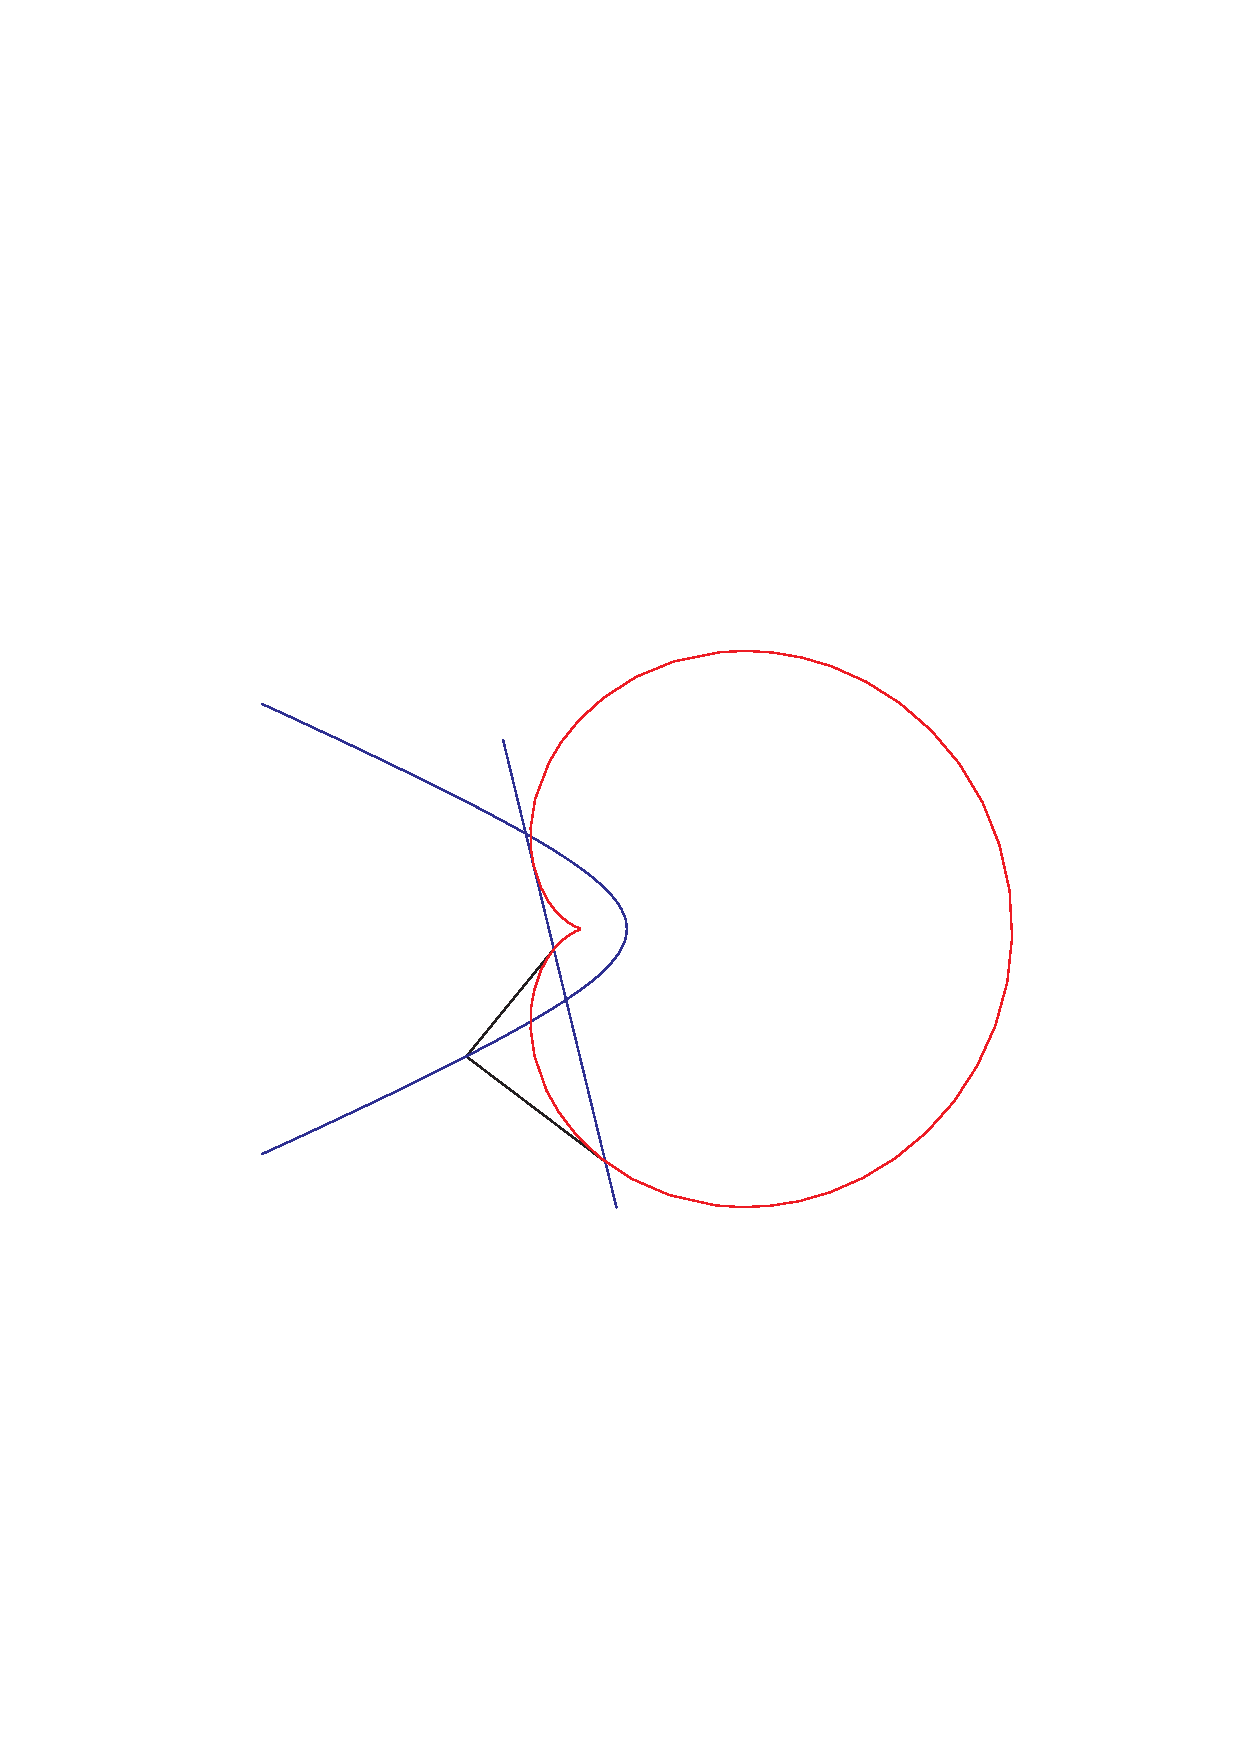
\includegraphics[width=8cm]{Ccardioid_1.pdf}
 % Ccardioid_1.pdf: 612x792 pixel, 72dpi, 21.59x27.94 cm, bb=0 0 612 792
\caption{Question 7.}
\end{figure}
\item Pour mettre l'équation précédente sous la forme d'une équation réduite de conique, on considère les termes en $x$ et $x^2$ comme le début d'un carré comme dans la méthode de factorisation canonique. On obtient une hyperbole d'équation réduite
\begin{equation*}
 \dfrac{\left( x - \dfrac{11}{10}\right)^2 }{\left( \dfrac{9}{10}\right)^2 }
- \dfrac{y^2}{\left( \dfrac{\sqrt{3}}{2\sqrt{5}}\right)^2}
= 1
\end{equation*}
d'axe focal $Ox$, de centre le point de coordonnées $(\frac{11}{10},0)$
\end{enumerate}

\subsubsection*{Annexe}
Les lignes de code suivantes permettent de réaliser avec Maple la substitution utilisée en question 4.
\begin{verbatim*}
A:=(3*tau^2-1)*(1-t^2)+(tau^3-3*tau)*2*t+(1+t^2)^2;
expand(subs(t=T+tau,A));
\end{verbatim*}
%
\newpage%
\section*{Problème 2}%
\addcontentsline{toc}{section}{Pb 2 : Droites, cercles : géométrie élémentaire avec des complexes. }%
\fancyhead[LO,RE]{Corrigés - Pb 2 : Droites, cercles : géométrie élémentaire avec des complexes. }%
\subsection*{Partie I.}
\begin{enumerate}
 \item
 \begin{enumerate}
   \item Le nombre complexe $j$ est défini comme la solution de partie imaginaire positive de l'équation $1 + z + z^2=0$. On sait aussi que
\[
  j = -\frac{1}{2} + i \frac{\sqrt{3}}{2} = e^{\frac{2i \pi}{3}},\hspace{0.5cm} j^3 = 1, \hspace{0.5cm} j^2 = \overline{j} = \frac{1}{j}, \hspace{0.5cm} |j| = 1.
\]
Comme $j^2$ est le conjugué de $j$:
\[
\frac{j^2 - j}{\overline{j^2 - j}} = \frac{\overline{j} - j}{j - \overline{j}} = -1.
\]
   \item  Avec les propriétés précédentes $|1-j| = |\overline{1-j}| = |1 - j^2|$ et $|1-j| = |j||1-j| = |j-j^2|$. On peut montrer que c'est $\sqrt{3}$.\newline
En multipliant par $u$, les modules sont multipliés par $|u|$ et les égalités sont conservées:
\begin{displaymath}
 |u-ju| = |ju-j^2u|=|j^2u -u|=\sqrt{3}|u|
\end{displaymath}
ce qui entraine que le triangle formé par les points d'affixes $u$, $ju$, $j^2u$ est équilatéral.

 \end{enumerate}

 \item
 \begin{enumerate}
   \item L'affixe du milieu de $M M'$ est $\frac{m + m'}{2}$. Comme $M$ et $M'$ sont symétriques, ce point est sur la droite $(A,B)$ donc il existe $\lambda$ réel tel que
\[
  \text{milieu de } MM' = A + \lambda \overrightarrow{AB} \Rightarrow
  \frac{m + m'}{2} = a + \lambda(b-a) \Rightarrow m + m' = 2a + 2 \lambda(b-a).
\]

   \item De manière analogue, $\overrightarrow{M M'}$ est orthogonal à $\overrightarrow{AB}$ car les points sont symétriques par rapport à $(AB)$. Cela se traduit par 
\[
  \frac{m' - m}{b-a} \in i \R \Rightarrow \exists \mu \in \R \text{ tq } m' - m = \mu i(b-a).
\]

   \item En ajoutant et en soustrayant les deux relations précédentes, on obtient
\[
\left\lbrace  
\begin{aligned}
  m' &= a + \lambda(b-a) + i \mu \frac{b-a}{2} \\
  m  &= a + \lambda(b-a) - i \mu \frac{b-a}{2}
\end{aligned} \right.
\Rightarrow
\left\lbrace 
\begin{aligned}
  \frac{m'-a}{b-a} &= \lambda + i  \frac{\mu}{2} \\
  \frac{m-a}{b-a}  &= \lambda - i \frac{\mu}{2}
\end{aligned} \right.
\Rightarrow \frac{m'-a}{b-a} = \overline{\left(\frac{m-a}{b-a}\right)}
\]
car $\lambda$ et $\mu$ sont réels.
 \end{enumerate}
 \item
 \begin{enumerate}
   \item Les relations $s(a)=a$ et $s(b)=b$ se traduisent par un système de deux équations aux inconnues $w_1$ et $w_2$
\[
  \left\lbrace
  \begin{aligned}
    \overline{a}\, w_1 + w_2 &= a \\ \overline{b}\,w_1 + w_2 &= b
  \end{aligned}
\right. .
\]
Son discriminant est
\[
  D = 
  \begin{vmatrix}
    \overline{a} & 1 \\ \overline{b} & 1
  \end{vmatrix}
= \overline{a} - \overline{b} \neq 0.
\]
Il admet un unique couple solution donné par les formules de Cramer
\[
  ( 
  \frac{
    \begin{vmatrix}
      a & 1 \\ b & 1
    \end{vmatrix}
  }{D} , 
  \frac{
    \begin{vmatrix}
      \overline{a} & a \\ \overline{b} & b
    \end{vmatrix}
  }{D} )
  = (\frac{a - b}{\overline{a - b}}, \frac{\overline{a}b - \overline{b}a}{\overline{a - b}}).
\]

   \item Pour exprimer $\frac{z' - a}{b -a}$, utilisons $m'=s(m)$, $a=s(a)$ et $b=s(b)$. \newline
   Comme $s(z) = w_1z + w_2$, les $w_2$ disparaissent dans les différence et il vient
\[
  \frac{z' - a}{b -a} = \frac{w_1 \bar{z} - w_1\bar{a}}{w_1 \bar{b} - w_1\bar{a}} = \overline{\left( \frac{z-a}{b-a}\right)}.
\]
Il s'agit de la même relation que celle obtenue en question 1 en échangeant $m$ et $z$. Les points $Z$ et $Z'$ sont donc symétriques par rapport à $(AB)$.
 \end{enumerate}
\end{enumerate}

\subsection*{Partie II.}
\begin{enumerate}
 \item Calculons les points demandés à partir de la relation de la question I.1.c. Présentons les résultats dans un tableau 
\begin{center}
\renewcommand{\arraystretch}{1.8}
\begin{tabular}{|c|c|c|c|} \hline
$(OA)$   & $(OB)$   & $(OC)$   & $(BC)$\\ \hline
$\frac{m_1-0}{1-0} = \overline{\left(\frac{m-0}{1-0}\right)}$ & 
$\frac{m_2-0}{j-0} = \overline{\left(\frac{m-0}{j-0}\right)}$ & 
$\frac{m_3-0}{j^2-0} = \overline{\left(\frac{m-0}{j^2-0}\right)}$ & 
$\frac{m_4-j}{j^2-j} = \overline{\left(\frac{m-j}{j^2-j}\right)}$\\ \hline
$m_1 = \overline{m}$ & $m_2 = j^2\, \overline{m}$ & $m_3 = j\,\overline{m}$ & $m_4 = -\overline{m} -1 $ \\ \hline
\end{tabular}
\end{center}
Certains calculs intermédiaires ont été effectués. par exemple
\[
  \frac{j}{\overline{j}} = \frac{j^4}{j^2} = j^2,\hspace{0.3cm}
  \frac{j^2}{\overline{j^2}} = \frac{j^2}{j} = j,\hspace{0.3cm}
  \frac{j^2 - j}{\overline{j^2 - j}} = \frac{\overline{j} - j}{j - \overline{j}} = -1.
\]
Les expressions de $m_1$, $m_2$, $m_3$ et la question I.1.b montrent que les points $M_1$, $M_2$, $M_3$ forment un triangle équilatéral.

\item On va montrer que $M_2$, $M_3$, $M_4$ sont alignés si et seulement si $M$ est sur le cercle de rayon $1$ et de centre le point d'affixe $-1$.\newline
Pour étudier la condition d'alignement de $M_2$, $M_3$, $M_4$ formons $\frac{m_2-m_4}{m_3-m_4}$ et utilisons la relation $1+j+j^2=0$ :
\begin{multline*}
 \frac{m_2-m_4}{m_3-m_4} = \frac{j^2\overline{m}+\overline{m}+1}{j\overline{m}+\overline{m}+1} 
= \frac{-j\overline{m}+1}{-j^2\overline{m}+1} \\ 
= \frac{1-jm -j\overline{m}+j^2|m|^2}{|-j^2\overline{m}+1|^2}
= \frac{1-2j\Re(m)+j^2|m|^2 }{|-j^2\overline{m}+1|^2}
\end{multline*}
Avec $x=\Re(m)$ et $y=\Im(m)$, l'expression précédente est réelle si et seulement si sa partie imaginaire est nulle c'est à dire:
\begin{displaymath}
 0=-\sqrt{3}x-\frac{\sqrt{3}}{2}(x^2+y^2) \Leftrightarrow (x+1)^2 + y^2 = 1
\end{displaymath}
ce qui démontre le résultat annoncé.\newline
Pour vérifier que $A$ est sur la droite, on considère la condition d'alignement de $A$ (d'affixe $1$) avec $M_2$ et $M_3$:
\[
 \frac{m_2 - 1}{m_3 - 1} = \frac{j^2 \overline{m} -1}{j \overline{m} -1} = \frac{m_3 - m_4}{m_2 - m_4} \in \R. 
\]
Ceci montre que $A$ est sur la même droite comme la figure de l'énoncé semble l'indiquer.

\item \begin{enumerate}
 \item Ici $M_2$, $M_3$, $M_4$ ne sont pas alignés et $\Omega$ est le centre du cercle circonscrit. On va prouver que $\Omega$ est  sur la droite $(OM_1)$ en montrant que $(OM_1)$ est la médiatrice de $M_2$ et $M_3$.\newline
Il suffit de montrer que $O$ et $M_1$ sont sur cette médiatrice. Comme $m_2=j^2\overline{m}$ et $m_3=j\overline{m}$, ils ont le même module donc le point $O$ est sur la médiatrice de $M_2$ et $M_3$.\newline
De même :
\begin{displaymath}
 |m_1 - m_2|=|1-j^2||m| = |1-\overline{j}||m| = |1-j||m| = |m_1-m_3| 
\end{displaymath}
donc $M_1$ est sur la médiatrice de de $M_2$ et $M_3$.

\item On note ici $m=\rho e^{i\theta}$ $\omega$ l'affixe de $\Omega$. Comme $\Omega\in (OM_1)$, il existe un réel $\lambda$ tel que $\omega=\lambda e^{-i\theta}$. \'Ecrivons que $|\omega-m_3|=|\omega-m_4|$, cela entraine :
\begin{multline*}
 |\lambda e^{-i\theta} -j\rho e^{-i\theta}| = |\lambda e^{-i\theta}+1 +\rho e^{-i\theta}| \Leftrightarrow
|\lambda -j\rho| = |\lambda+\rho +e^{i\theta}| \\
\Leftrightarrow (\lambda + \frac{\rho}{2})^2 + \frac{3}{4}\rho^2 = (\lambda + \rho + \cos \theta)^2 + \sin^2\theta \\
\Leftrightarrow  \lambda(\rho + 2\cos\theta)+1+2\rho\cos \theta = 0
\end{multline*}
d'où l'expression de $\lambda$ et celle de $\omega$ demandée par l'énoncé.

\item Pour calculer $R$, on utilise le point $M_3$.
\begin{multline*}
 R = |m_3-\omega| = \left\vert j\rho e^{-i\theta} + \frac{1+2\rho\cos \theta}{\rho +2\cos \theta}e^{-i\theta}\right\vert
= \left\vert j\rho  + \frac{1+2\rho\cos \theta}{\rho +2\cos \theta}\right\vert\\
\Rightarrow R^2 
= \rho^2 + \left(\frac{1+2\rho\cos \theta}{\rho +2\cos \theta}\right)^2 + 2\rho\,\frac{1+2\rho\cos \theta}{\rho +2\cos \theta}\Re(j)\\
= \rho^2 + \left(\frac{1+2\rho\cos \theta}{\rho +2\cos \theta}\right)\left( \frac{1+2\rho\cos \theta}{\rho +2\cos \theta} - \rho\right)
= \rho^2 + \frac{(1 + 2\rho\cos \theta)(1-\rho^2)}{(\rho + 2\cos \theta)^2}.
\end{multline*}
\end{enumerate}

\item On va montrer que $\Gamma$ est l'union du cercle unité et de la droite $(BC)$.\newline
Le cercle circonscrit aux points $M_1$, $M_2$, $M_3$ d'affixes $m_1 = \overline{m}$, $m_2 = j^2\overline{m}$ , $m_3 = j\overline{m}$ est de centre $O$ et de rayon $|m|=\rho$. D'après la question 3.c., les rayons des deux cercles circonscrits sont égaux si set seulement si :
\begin{displaymath}
 R^2 = \rho^2 \Leftrightarrow \frac{(1+2\rho\cos\theta)(1-\rho^2)}{(\rho+2\cos \theta)^2} = 0
\end{displaymath}
c'est à dire si et seulement si on est dans une des deux situations suivantes:
\[
\begin{aligned}
  &1+2\rho\cos\theta = 1+2x=0 &\Leftrightarrow& M \in (BC)\\
  &\rho =1 &\Leftrightarrow& M \text{ sur le cercle unité}.
\end{aligned}
\]
On remarque de plus que dans le premier cas, $M = M_4$ car $M \in (BC)$ et $\Omega= O$ d'après la question 3.b. Les deux cercles circonscrits ont le même centre et le même rayon, ils sont confondus.\newline
La figure 4 complétée en figure \ref{fig:Ccomp2_1} présente le cas où $M$ est à sur $(BC)$. Dans ce cas les deux cercles sont confondus (de centre $O$).
\begin{figure}
 \centering
\includegraphics[width=5cm]{Ccomp2_1}
\caption{$M\in (BC)$} \label{fig:Ccomp2_1}
\end{figure} \newline
La figure 5 complétée en figure \ref{fig:Ccomp2_2} présente le cas où $M$ est sur le cercle unité. Les deux cercles sont alors de même rayon mais distincts.
\begin{figure}
 \centering
\includegraphics[width=5cm]{Ccomp2_2}
\caption{$M$ sur le cercle unité} \label{fig:Ccomp2_2}
\end{figure}
\end{enumerate}
%
\newpage%
\section*{Problème 3}%
\addcontentsline{toc}{section}{Pb 3 : Propriété des nombres complexes. Etude d'une famille d'équations }%
\fancyhead[LO,RE]{Corrigés - Pb 3 : Propriété des nombres complexes. Etude d'une famille d'équations }%
\begin{enumerate}
 \item Les résultats sont présentés dans un tableau
\begin{displaymath}
% use packages: array
\renewcommand{\arraystretch}{2}
\begin{array}{c|c|c}
n &  E_0(n,a) & E_1(n,a) \\ 
\hline n=2 & 
\begin{array}{c}
 z^2 + a^2=0 \\
 \{ia,-ia\}
\end{array}

&
\begin{array}{c}
 2za=0  \\ \{ 0 \}
\end{array}\\
\hline n=3 & 
\begin{array}{c}
3z^2a+a^3=0 \\ \{ \frac{ia}{\sqrt{3}}, -\frac{ia}{\sqrt{3}}\}
\end{array}

&
\begin{array}{c}
 z^3+3za^2=0 \\ \{0, i\sqrt{3}a, - i\sqrt{3}a\}
\end{array}


  \\ 
\hline n=4 &
\begin{array}{c}
 z^4+6z^2a^2+a^4=0 \\ \mathcal S
\end{array}
 & 
\begin{array}{c}
4z^3a+4za^3=0 \\ \{ 0,ia, -ia\}
\end{array}
\end{array}
\end{displaymath}
avec
\begin{displaymath}
 \mathcal S = \left\lbrace ia\sqrt{3+2\sqrt{2}}, -ia\sqrt{3+2\sqrt{2}}, ia\sqrt{3-2\sqrt{2}}, -ia\sqrt{3-2\sqrt{2}},  \right\rbrace 
\end{displaymath}
L'ensemble $\mathcal S $ s'obtient en prenant les racines carrées des solutions de l'équation 
\begin{displaymath}
z^2+6u^2z+a^4 
\end{displaymath}
d'inconnue $z$.
On peut remarquer que $(1+\sqrt 2)^2 = 3+2\sqrt{2}$ et donc remplacer $\sqrt{3+2\sqrt{2}}$ par $1+\sqrt 2$ dans l'expression de $\mathcal S$.
\item Dans cette question, le point important est que l'on puisse écrire $\lambda^n=\lambda^k \lambda^{n-k}$. Comme $\lambda\neq 0$, on peut multiplier par $\lambda^n$ donc $w$ est solution de $E_0(n,a)$ si et seulement si
\begin{displaymath}
 \lambda^n \sum_{k\in \mathcal P _n}\binom{n}{k}w^ka^{n-k}=0
\Leftrightarrow
\sum_{k\in \mathcal P _n}\binom{n}{k}(\lambda w)^k(\lambda a)^{n-k}=0
\end{displaymath}
C'est à dire lorsque $\lambda w$ est solution de $E_0(n,\lambda a)$. Le raisonnement est exactement le même pour $E_1(n,a)$.
\item 
\begin{enumerate}
 \item 
   \begin{itemize}
     \item Si $w=-1$ l'équation n'admet pas de solution.
     \item Si $w\neq -1$ l'équation admet une unique solution
\begin{displaymath}
 a\frac{w-1}{w+1}
\end{displaymath}
   \end{itemize}
\item En utilisant $e^{i\frac{\alpha}{2}}$ comme dans le cours, on obtient
\begin{displaymath}
 \frac{w-1}{w+1} = i\tan \frac{\alpha}{2}
\end{displaymath}
\item L'ensemble cherché est formé par les solutions des équations 
\begin{displaymath}
 \frac{a+z}{a-z} = u
\end{displaymath}
pour les $u$ de $\U_n$.
\begin{itemize}
 \item Lorsque $n$ est impair, $-1$ n'est pas dans $\U_n$ donc d'après a. et b. l'ensemble des solutions est
\begin{displaymath}
 \left\lbrace ia \tan \frac{k\pi}{n}, n\in \{0,\cdots n-1\}\right\rbrace 
\end{displaymath}
\item  Lorsque $n$ est pair, $-1$ est pas dans $\U_n$ donc d'après a. et b. il y a une solution de moins. L'ensemble des solutions est
\begin{displaymath}
 \left\lbrace ia \tan \frac{k\pi}{n}, n\in \{0,\cdots n-1\}-\{\frac{n}{2}\}\right\rbrace 
\end{displaymath}
\end{itemize}
\item Le développement (selon la formule du binôme) de $(-z+a)^n$ s'obtient à partir de celui de $(z+a)^n$ en affectant chaque coefficient de $z^k$ d'un $-1$ lorsque $k$ est impair. On en déduit que
\begin{displaymath}
 (z+a)^n - (-z+a)^n = 2 \sum_{k\in \mathcal I _n}\binom{n}{k}w^k a^{n-k}
\end{displaymath}
puis que les solutions de $E_1(n,a)$ sont les mêmes que celles de l'équation du c.

\end{enumerate}

\item \begin{enumerate}
 \item En développant selon la formle du binôme, on obtient
\begin{eqnarray*}
 \Re \left( (x+iy)^n\right)  &=& \sum_{k\in \mathcal P _n}\binom{n}{k}x^{n-k} (iy)^{k} \\
 i \Im \left( (x+iy)^n\right)  &=& \sum_{k\in \mathcal I _n}\binom{n}{k}x^{n-k} (iy)^{k}
\end{eqnarray*}
\item On peut appliquer ces formules avec $x=\cos \theta$ et $y=\sin \theta$, comme de plus
\begin{displaymath}
 (\cos \theta + i\sin\theta)^n = e^{in\theta}
\end{displaymath}
On en déduit
\begin{eqnarray*}
 \cos n\theta  &=& \sum_{k\in \mathcal P _n}\binom{n}{k}(\cos \theta)^{n-k} (i\sin \theta)^{k} \\
 i \sin n\theta  &=& \sum_{k\in \mathcal I _n}\binom{n}{k}(\cos \theta)^{n-k} (i\sin \theta)^{k}
\end{eqnarray*}
En mettant $(\cos \theta )^n$ en facteur, on obtient :
\begin{eqnarray*}
\frac{\cos n\theta}{(\cos \theta )^n}   &=& \sum_{k\in \mathcal P _n}\binom{n}{k}\left( \frac{i\sin \theta}{\cos \theta}\right) ^{k} \\
 i \frac{\sin n\theta}{(\cos \theta )^n}   &=& \sum_{k\in \mathcal I _n}\binom{n}{k}\left( \frac{i\sin \theta}{\cos \theta}\right) ^{k} 
\end{eqnarray*}
\item D'après la question précédente, les nombres $i\tan \theta$ pour lesquels $\sin n\theta = 0$ sont des solutions de $E_1(n,1)$ (avec le paramêtre $a=1$). D'après la question 2. les nombres $ai\tan \theta$ pour lesquels $\sin n\theta = 0$ sont des solutions de $E_1(n,a)$. On retrouve donc l'ensemble
\begin{displaymath}
\left\lbrace ia \tan \frac{k\pi}{n}, n\in \{0,\cdots n-1\}-\{\frac{n}{2}\}\right\rbrace 
\end{displaymath}

\item D'après la question 4.b., les nombres $i\tan \theta$ pour lesquels $\cos n\theta = 0$ sont des solutions de $E_0(n,1)$ (avec le paramêtre $a=1$). Comme on en trouve le bon nombre suivant la parité de $n$ ce sont toutes les solutions. D'après la question 2., les solutions de $E_0(n,a)$ sont les $ai\tan \theta$ pour lesquels $\cos n\theta = 0$.
\end{enumerate}

\end{enumerate}
%
\newpage%
\section*{Problème 4}%
\addcontentsline{toc}{section}{Pb 4 : Ellipse: ``bande de papier'' et cercles de Chasles.}%
\fancyhead[LO,RE]{Corrigés - Pb 4 : Ellipse: ``bande de papier'' et cercles de Chasles.}%
\begin{figure}[ht]
 \centering
 \includegraphics{Cconi1_1.pdf}
 % Cconi1_1.pdf: 302x283 pixel, 72dpi, 10.65x9.98 cm, bb=0 0 302 283
\caption{Construction de quelques points}
\label{fig:Cconi_1}
\end{figure} 
\begin{figure}[ht]
 \centering
\input{Cconi1_2.pdf_t}
\caption{Cercles de Chasles}
\label{fig:Cconi_2}
\end{figure}

\begin{enumerate}
 \item Voir la figure.
\item \begin{enumerate}
 \item Par définition, $0$, $P$, $I$, $Q$ est un rectangle donc les diagonales sont égales :
\begin{displaymath}
 OI = PQ =a+b
\end{displaymath}
 
\item Les coordonnées de $I$ s'obtiennent de la question précédente et de la définition de $\theta$, celles de $P$ et $Q$ s'en déduisent immédiatement :
\begin{align*}
 \text{coordonnées de $I$} &: ((a+b)\cos \theta , (a+b)\sin \theta) \\
 \text{coordonnées de $P$} &: ((a+b)\cos \theta , 0) \\
 \text{coordonnées de $Q$} &: (0 , (a+b)\sin \theta) 
\end{align*}
Par définition, $M$ est le barycentre de $(P,a)$ et de $(Q,b)$ donc
\begin{displaymath}
 (a+b)\overrightarrow{OM} = a\overrightarrow{OP} +  b\overrightarrow{OQ}
\end{displaymath}
Les coordonnées de $M$ sont donc
\begin{displaymath}
 (a\cos \theta , b \sin \theta)
\end{displaymath}
\item D'après la question précédente $\mathcal E$ est une ellipse.
\end{enumerate}
\item Voir la figure. Le point $I(\theta)$ est sur le cercle $\Gamma$, le point $J(\theta)$ est sur le cercle $\Gamma '$.
\begin{align*}
 \text{coordonnées de $I(\theta)$} &:  ((a+b)\cos \theta , (a+b)\sin \theta) \\
 \text{coordonnées de $J(\theta)$} &:  ((a-b)\cos \theta , (-a+b)\sin \theta) \\
 \text{coordonnées du milieu} &: (a\cos \theta , b\sin \theta) 
\end{align*}
On en déduit que le milieu est le point $M$ de la question 2.\newline
Les coordonnées de $\overrightarrow{I(\theta)J(\theta)}$ sont 
\begin{displaymath}
 (-2b\cos \theta , -2a \sin \theta)
\end{displaymath}
La tangente en $M(\theta)$ à l'ellipse $\mathcal E$ est portée par la dérivée dont les coordonnées sont :
\begin{displaymath}
 (-a\sin \theta , b\cos \theta)
\end{displaymath}
Ce vecteur est orthogonal à $\overrightarrow{I(\theta)J(\theta)}$ donc $(IJ)$ est la normale en $M$ à l'ellipse.
\end{enumerate}
%
\newpage%
\section*{Problème 5}%
\addcontentsline{toc}{section}{Pb 5 : Coniques, enveloppes, cercles directeurs.}%
\fancyhead[LO,RE]{Corrigés - Pb 5 : Coniques, enveloppes, cercles directeurs.}%
\subsubsection*{Partie I.}
\begin{figure}
	\begin{center}
	\input{Cconi2_1.pdf_t}
	\end{center}
\caption{I.1. Cas $0<c<a$.}
\label{fig:Cconi2_1}
\end{figure} 
\begin{figure}
	\begin{center}
	\input{Cconi2_2.pdf_t}
	\end{center}
\caption{I.1.Cas $0<c=a$.}
\label{fig:Cconi2_2}
\end{figure} 
\begin{figure}
	\begin{center}
	\input{Cconi2_3.pdf_t}
	\end{center}
\caption{I.1. Cas $0<a<c$.}
\label{fig:Cconi2_3}
\end{figure} 

\begin{enumerate}
 \item Voir Fig. \ref{fig:Cconi2_1}, Fig. \ref{fig:Cconi2_2}, Fig.\ref{fig:Cconi2_3} .
 \item Lorsque $c=a$, comme $B$ et $C_\theta$ sont sur le même cercle (Fig. 2.) de centre $A$, l'intersection de la médiatrice de $[BC_\theta]$ avec la droite $(AC_\theta)$ est toujours $A$.
\begin{displaymath}
 \mathcal C = \{A\}
\end{displaymath}
\item Les calculs sont évidents :
\begin{align*}
 z(A)=0 &,& z(B)=2c &,& z(C_\theta)=2ce^{i\theta} &,& z(H_\theta)=c+ae^{i\theta} 
\end{align*}
Lorsque $\theta$ varie, le point $H_\theta$ décrit le cercle de centre de point de coordonnées $(c,0)$ et de rayon $a$.
\item 
\begin{enumerate}
 \item Comme $M_\theta$ est sur la droite $(AC_\theta)$, il existe un réel $\lambda$ tel que
\begin{displaymath}
 z(M_\theta) = \lambda e^{i\theta}
\end{displaymath}
\item \'Ecrivons l'orthogonalité de $\overrightarrow{H_\theta M_\theta}$ et $\overrightarrow{BC_\theta}$ avec les affixes complexes :
\begin{displaymath}
 \frac{\lambda e^{i\theta} -c - a e^{i\theta}}{2ae^{i\theta}-2c} \in i\R
\end{displaymath}
Le $2$ qui se met en facteur au dénominateur ne change pas la condition d'être imaginaire pur. On le fait donc disparaitre. On multiplie par $e^{-i\theta}$ en haut et en bas. La condition devient :
\begin{displaymath}
 \frac{\lambda -a -c e^{-i\theta} }{a-ce^{-i\theta}} \in i\R
\end{displaymath}
Si on multiplie en haut et en bas par la quantité conjuguée du dénominateur, celui ci devient un réel sctrictement positif et peut donc disparaitre de la condition. On obtient alors :
\begin{displaymath}
 (\lambda -a -c e^{-i\theta})(a-ce^{i\theta}) \in i\R
\end{displaymath}
\item Le point $M_\theta$ existe lorsque la médiatrice de $BC_\theta$ coupe $AC_\theta$. Le point n'est pas correctement défini lorsque ces droites sont parallèles c'est à dire lorsque le triangle $AC_\theta B$ est rectangle en $C_\theta$. Cela ne peut se produire que si 
\begin{align*}
 c>a & & \cos \theta =\dfrac{a}{c}
\end{align*}
Il existe donc un point $M_\theta$
\begin{itemize}
 \item pour tous les $\theta$ lorsque $c<a$
\item pour tous les $\theta$ autres que $\theta_0$ et $-\theta_0$ lorsque $c>a$.
\end{itemize}
Calculons $M_\theta$ dans ces cas.\newline
D'après b., l'affixe de $M_\theta$ est de la forme $\lambda e^{i\theta}$ avec $\lambda$ vérifiant :
\begin{displaymath}
 (\lambda -a-ce^{i\theta})(a-ce^{i\theta})\in i\R
\end{displaymath}
\'Ecrivons que la partie rélle est nulle :
\begin{displaymath}
 (\lambda - a-c \cos \theta)(a-c \cos \theta)-(c\sin \theta)(-c\sin \theta)=0\Leftrightarrow
\lambda = \dfrac{a^2-c^2}{a-c\cos \theta}
\end{displaymath}
\end{enumerate}
\item Lorsque $c<a$, pour tous les $\theta$ : $\lambda >0$.\newline
Lorsque $a<c$, on peut former le tableau :
\begin{displaymath}
\begin{array}{ccccccc}
 -\pi &   & -\theta_0 &   & \theta_0 &   & \pi \\ \hline
      & - &   \Vert  & + & \Vert    & - &  
\end{array}
 \end{displaymath}

\end{enumerate}
\subsubsection*{Partie II.}
\begin{figure}[ht]
 \centering
\input{Cconi2_4.pdf_t}
\caption{Définition bifocale : ellipse $c<a$}
\label{fig:Cconi2_4}
\end{figure}
\begin{figure}[ht]
 \centering
\input{Cconi2_5.pdf_t}
\caption{Définition bifocale : branches d'hyperbole $a<c$}
\label{fig:Cconi2_5}
\end{figure}
\begin{enumerate}
 \item Par construction, le point $M_\theta$ est sur la médiatrice de $BC_\theta$ donc $M_\theta C_\theta=M_\theta B$. 
\item D'après les questions précédentes, l'affixe de $M_\theta$ est $\lambda e^{i\theta}$ avec 
\begin{displaymath}
 \lambda = \dfrac{a^2-c^2}{a-\cos \theta}
\end{displaymath}
L'ordre dans lequel sont placés les points alignés $A$, $M_\theta$, $C_\theta$ dépend du signe de $\lambda$ et de $2a-\lambda$.\newline
Dans le cas où $c<a$, ces deux réels sont strictement positifs. Les points $A$, $M_\theta$, $C_\theta$ sont alignés dans cet ordre avec
\begin{displaymath}
 AM_\theta + BM_\theta = AM_\theta + M_\theta C_\theta = 2a
\end{displaymath}
Le point $M_\theta$ décrit alors une ellipse de foyers $A$ et $B$ et de grand axe $2a$ (Fig.\ref{fig:Cconi2_4})\newline
Lorsque $a<c$, le point $M_\theta$ décrit les branches d'une hyperbole de foyers $A$ et $B$ (Fig. \ref{fig:Cconi2_5}). Le détail est présenté dans un tableau:
\begin{displaymath}
\begin{array}{cccccccc}
             &-\pi &   & -\theta_0 &   & \theta_0 &   & \pi \\ \hline
     \lambda & |   & - &   \Vert  & + & \Vert    & - &  \\ \hline
 2a- \lambda & |   & + &   \Vert  & - & \Vert    & + &  \\ \hline
\text{alignement} & |   & MAC &   \Vert  & ACM & \Vert    & MAC &  \\ \hline
2a= & |   & MB -MA &   \Vert  & MA-MB & \Vert &  MB -MA &  
\end{array}
 \end{displaymath}
\end{enumerate}

\begin{figure}[ht]
 \centering
 \includegraphics[width=7.5cm]{Cconi2_7.pdf}
 % Cconi2_7.pdf: 595x842 pixel, 72dpi, 20.99x29.70 cm, bb=0 0 595 842
\caption{III.3.b Enveloppe d'une famille de droites}
\label{fig:Cconi2_7}
\end{figure}
\subsubsection*{Partie III.}
\begin{enumerate}
 \item L'intersection des deux droites est régie par un système de deux équations linéaires dont le déterminant est 
\begin{displaymath}
 U(t)V^\prime(t)-U^\prime(t)V(t)\neq 0
\end{displaymath}
Ce système admet donc pour chaque $t$ un unique couple solution. On le note $(a(t),b(t))$.
\item Il ne faut \emph{surtout pas} chercher à préciser lescoordonnées $(a(t),b(t))$ du point $f(t)$.  \'Ecrivons que $f(t)\in \Delta_t$ puis dérivons cette relation :
\begin{eqnarray*}
 0&=& U(t)a(t)+V(t)b(t)+W(t) \\
0 &=& \left( U^\prime(t)a(t)+V^\prime(t)b(t)+W^\prime(t)\right)  + U(t)a^\prime(t)+V(t)b^\prime(t)
\end{eqnarray*}
La parenthèse est nulle car $f(t)\in \Delta^\prime _t$. Le reste de la relation traduit l'orthogonalité de $\overrightarrow{f^\prime}(t)$ avec le vecteur de coordonnées $(U(t),V(t))$. Or ce vecteur est normal à $\Delta_t$ (d'après son équation), on en déduit donc que $\overrightarrow{f^\prime}(t)$ est dans la direction de $\Delta_t$ ce qui assure que c'est la tangente car elle contient $f(t)$.
\item
\begin{enumerate}
 \item Pour former l'équation de $\Delta_t$, on écrit la nullité du produit scalaire des vecteurs de coordonnées
\begin{align*}
 \begin{pmatrix}
  x-R\cos t \\ y-R\sin t
 \end{pmatrix}
& &
\begin{pmatrix}
 R\cos t -s \\ R\sin t
\end{pmatrix}
\end{align*}
On obtient après calculs :
\begin{displaymath}
 \text{équation de $\Delta_t$ } : 
(R\cos t -s)x+R\sin t y -R^2+Rs\cos t =0
\end{displaymath}

\item Les coordonnées de $f(t)$ sont les solutions du système
\begin{displaymath}
 \left\lbrace 
\begin{aligned}
 (R\cos t -s)x+R\sin t y -R^2+Rs\cos t =& 0\\
 -R\sin t x +R \cos t y -Rs\sin t =&0
\end{aligned}
\right. 
\end{displaymath}
 Que l'on résoud (après division de la deuxième équation par $-R$) à l'aide des formules de Cramer. On obtient
\begin{align*}
 x=R\,\dfrac{s-R\cos t}{s\cos t -R} & & y=(s^2-R^2)\dfrac{\sin t}{s\cos t -R}
\end{align*}
Sur la figure \ref{fig:Cconi2_7}, on voit se dessiner une ellipse.
\end{enumerate}

\end{enumerate}

\subsubsection*{Partie IV.}
\begin{enumerate}
 \item Par définition, $\mathcal D_\theta$ est la médiatrice de $B$ et de $C_\theta$. Pour obtenir l'équation, écrivons l'égalité des carrés des distance à ces deux points
\begin{displaymath}
 (x-2a\cos \theta)^2+(y-2a\sin \theta)^2=(x-2c)^2+y^2
\end{displaymath}
après simplifications 
\begin{align*}
 \text{équation de $\mathcal D_\theta$ : } & &
(c-a\cos \theta)x - a\sin\theta y +a^2-c^2 =0
\end{align*}

\item On forme l'équation de $\mathcal D'_\theta$ en dérivant les coefficients
\begin{displaymath}
 a\sin \theta x-a\cos \theta y =0
\end{displaymath}
On résout le système constitué par les deux équations avec les formules de Cramer:
\begin{align*}
 \begin{vmatrix}
  c-a\cos\theta & -a\sin \theta \\
  \sin \theta & -\cos\theta
 \end{vmatrix} =& -c\cos \theta +a \\
\begin{vmatrix}
 -a^2+c^2 & -a\sin \theta \\
0 & -\cos \theta
\end{vmatrix}=&(a^2-c^2)\cos\theta \\
\begin{vmatrix}
 c-a\cos\theta &-a^2+c^2 \\
\sin \theta & 0
\end{vmatrix}=&(a^2-c^2)\sin \theta
\end{align*}
Les coordonnées du point d'intersection sont donc
\begin{displaymath}
 \left( \dfrac{a^2-c^2}{a-c\cos\theta}\cos \theta , \dfrac{a^2-c^2}{a-c\cos\theta}\sin \theta \right) 
\end{displaymath}
ce qui correspond bien à l'affixe complexe de $M_\theta$ trouvée en I. D'après la partie III, la courbe $\mathcal C$ est l'enveloppe des droites $\mathcal D_\theta$. Chacune de ces droites est donc tangente à $\mathcal C$ en $M_\theta$.
\item La distance d'un point à une droite s'obtient en utilisant l'équation de cette droite (obtenue en 1.)
\begin{displaymath}
 d(A,\mathcal D_\theta)d(B,\mathcal D_\theta)
=\dfrac{(a^2-c^2)\left((c-a\cos\theta)2c+a^2-c^2 \right) }{(c-a\cos\theta)^2+a^2\sin^2\theta}
=a^2-c^2
\end{displaymath}

\item Comme $\mathcal D_\theta$ est tangente à la conique et orthogonale à $C_\theta B$, la projection orthogonale sur la tangente en $M_\theta$ est $H_\theta$. L'affixe de ce point est 
\begin{displaymath}
 c+ae^{i\theta}
\end{displaymath}
Il décrit un cercle de centre $B$ et de rayon $a$. La podaire d'un foyer sur une conique (ellipse ou hyperbole) est donc un cercle. Le cas d'une parabole est examiné dans la dernière partie.
\end{enumerate}

\begin{figure}[ht]
 \centering
\input{Cconi2_6.pdf_t}
\caption{Podaire d'un foyer sur une parabole}
\label{fig:Cconi2_6}
\end{figure}
\subsubsection*{Partie V.}
\begin{enumerate}
\item\begin{enumerate}
 \item Pour obtenir l'équation cartésienne de $\mathcal P$, on écrit que $M$ de coordonnées $(x,y)$ est sur $\mathcal P$ si et seulement si $d(M,\mathcal D)=MF$
\begin{displaymath}
 \vert x+\dfrac{p}{2}\vert=\sqrt{(x-\dfrac{p}{2})^2+y^2}
\Leftrightarrow
(x+\dfrac{p}{2})^2=(x-\dfrac{p}{2})^2+y^2
\Leftrightarrow
y^2=2px
\end{displaymath}
 \item Les coordonnées de $M_u$ vérifient l'équation cartésienne de la parabole.
\end{enumerate}
 
\item On connait les coordonnées de $M_u$ et de sa dérivée :
\begin{align*}
 M_u:(2pu^2,2pu) & & \overrightarrow M_u :(4pu,2p)
\end{align*}
On en déduit l'équation de la tangente en $M_u$:
\begin{align*}
\text{équation de $\mathcal T_u$ : }& &
 \begin{vmatrix}
  x-2pu^2 & 2u \\
y-2pu & 1
 \end{vmatrix}=0
\Leftrightarrow
x-2uy+2pu^2=0
\end{align*}

\item Les coordonnées de $K_u$ sont $(-\frac{p}{2},2pu)$, écrivons encore une fois les distances à la droite avec son équation:
\begin{align*}
 d(F,\mathcal T_u)=&\dfrac{\frac{p}{2}+2pu^2}{\sqrt{1+4u^2}}\\
d(K_u,\mathcal T_u)=&\dfrac{\left\vert -\frac{p}{2}-2u(2pu)+2pu^2 \right\vert}{\sqrt{1+4u^2}}
= d(F,\mathcal T_u)
\end{align*}
On en déduit que $\mathcal T_u$ est la médiatrice de $[K_u,F]$.
\item Comme $\mathcal T_u$ est la médiatrice de $[K_u,F]$, le projeté $H_u$ de $F$ sur la tangente $\mathcal T_u$ est le milieu de $[F,K_u]$. Par conséquent, comme $F$ a pour coordonnées $(\frac{p}{2},0)$, lorsque $K_u$ décrit $\mathcal D$ (d'équation $x=\frac{p}{2}$), le point $H_u$ décrit l'axe $Oy$ (Fig. \ref{fig:Cconi2_6}).
\end{enumerate}

\clearpage%
\newpage%
\section*{Problème 6}%
\addcontentsline{toc}{section}{Pb 6 : Strophoïde et cissoïde}%
\fancyhead[LO,RE]{Corrigés - Pb 6 : Strophoïde et cissoïde}%
Dans tout le corrigé, on désignera par $\overrightarrow{e}_\theta$ le vecteur dont les coordonnées sont $(\cos \theta , \sin \theta)$ dans la base $\overrightarrow{i},\overrightarrow{j}$ attachée au repère fixé.
\begin{figure}[ht]
 \centering
 \input{Ccubcirc_1.pdf_t}
 \caption{Stropho{\"i}de droite}
 \label{fig:Ccubcirc_1} 
\end{figure}

\subsection*{PARTIE I. \'Etude de la stropho{\"i}de droite}
\begin{enumerate}
 \item Les coordonnées du centre du cercle sont $(-2a, 0)$, son rayon est $2a$. On en déduit l'équation cartésienne. On obtient l'expression en coordonnées polaires de cette équation cartésienne en remplaçant $x$ par $\rho \cos \theta$ et $y$ par $\rho \sin \theta$.
\begin{displaymath}
 (x+2a)^2+y^2 = 4a^2 \Leftrightarrow x^2+y^2+4ax=0
\Leftrightarrow \rho^2 + 4a\rho \cos \theta =0 
\Leftrightarrow \rho(\rho + 4a \cos \theta) =0 
\end{displaymath}
Il est utile de remarquer que l'équation polaire du cercle privé de $O$ est :
\begin{displaymath}
 \rho + 4a \cos \theta =0
\end{displaymath}
\item Comme le point $M(\theta)$ est sur le cercle $C$ et la droite passant par l'origine dirigée par $\overrightarrow{e}_\theta$, on obtient immédiatement :
\begin{displaymath}
 M(\theta) = O +\rho \overrightarrow{e}_\theta
= O  -4a\cos \theta \overrightarrow{e}_\theta
\end{displaymath}
De même, on forme l'équation cartésienne puis l'expression en coordonnées polaires de l'équation de la droite :
\begin{displaymath}
 x=2a \Leftrightarrow \rho \cos \theta =2a
\end{displaymath}
On en déduit $H(\theta)$
\begin{displaymath}
 H(\theta) = O +\rho \overrightarrow{e}_\theta
= O  +\dfrac{2a}{\cos \theta} \overrightarrow{e}_\theta
\end{displaymath}
puis le point $I(\theta)$ milieu des deux précédents.
\begin{displaymath}
 I(\theta)=O + \left( \dfrac{a}{\cos \theta} -2a\cos \theta \right)\overrightarrow{e}_\theta 
= O + a \dfrac{1-2\cos^2 \theta}{\cos \theta}\overrightarrow{e}_\theta 
= O - a \dfrac{\cos 2\theta}{\cos \theta}\overrightarrow{e}_\theta 
\end{displaymath}

\item L'expression de $r$ conduit à :
\begin{align*}
 &r(\theta+2\pi) = r(\theta) & &I(\theta +2\pi) = I(\theta)  \\
 &r(\theta+ \pi) = -r(\theta) & &I(\theta + \pi) = I(\theta)  \\
 &r(-\theta) = r(\theta) & &I(-\theta ) = s_{Ox}(I(\theta))  \text{ avec $s_{Ox}$ symétrie par rapport à $Ox$}
\end{align*}
La fonction $I$ étant $\pi$-périodique, on peut se limiter à $[-\frac{\pi}{2} +\frac{\pi}{2}]$. L'image de $[-\frac{\pi}{2},0]$ s'obtient par symétrie par rapport à $Ox$ à partir de l'image de $[0,\frac{\pi}{2}]$. On étudiera la courbe sur $E = [0,\frac{\pi}{2}]$.

\item Il est évident que, au voisinage de $\frac{\pi}{2}$, 
\begin{displaymath}
 r(\theta)\sin(\theta - \dfrac{\pi}{2}) = -r(\theta)\cos \theta = a\cos 2\theta 
\rightarrow -a
\end{displaymath}
On en déduit $x(I(\theta)) = r(\theta)\cos \theta \rightarrow a$. La courbe admet donc comme asymptote la droite d'équation $x=a$.
\item Le signe de $r$ est donné dans le tableau suivant :
\renewcommand{\arraystretch}{1.8}
\begin{displaymath}
 \begin{array}{|c|ccccc|} \hline
          & 0   &   & \dfrac{\pi}{4} &   & \dfrac{\pi}{2} \\ \hline
r(\theta) & -a  & - &       0        & + &  \Vert \\ \hline
\end{array}
\end{displaymath}
Ce tableau montre que pour $\theta$ entre $0$ et $\frac{\pi}{4}$, le point $I(\theta)$ est dans le secteur angulaire symétrique de $\overrightarrow{e}_\theta$ par rapport au point $O$. La figure \ref{fig:Ccubcirc_1} présente le cercle $C$, la droite $D$ et le support de $I$.
\item Notons (abusivement) $x=x(I(\theta))$ et $y=y(I(\theta))$. On peut alors écrire :
\begin{align*}
 x=-a\cos2\theta = a -2a\cos^2\theta 
&\Rightarrow  \cos^2 \theta = \dfrac{a-2x}{2a} \\
y=-a\dfrac{\cos 2\theta}{\cos \theta}\sin \theta =x\tan \theta 
&\Rightarrow \tan \theta =\dfrac{y}{x} \\
1+ \tan^2 \theta = \dfrac{1}{\cos^2 \theta}
&\Rightarrow \left( \dfrac{y}{x}\right)^2 = \dfrac{2a}{a-x}-1=\dfrac{a+x}{a-x} 
\end{align*}
On en déduit que le suppoort de la courbe paramétrée $I$ est inclus dans la courbe d'équation cartésienne
\begin{displaymath}
 (a-x)y^2 = x^2(a+x)
\end{displaymath}

\end{enumerate}

\begin{figure}[ht]
 \centering
 \input{Ccubcirc_2.pdf_t}
 \caption{Cisso{\"i}de droite}
 \label{fig:Ccubcirc_2} 
\end{figure}
\subsection*{PARTIE II. \'Etude de la cisso{\"i}de droite}
\begin{enumerate}
\item L'équation cartésienne du cercle $S$ est immédiate :
\begin{displaymath}
 (x+a)^2+y^2=a^2 \Leftrightarrow x^2 +2ax +y^2 =0
\end{displaymath}

\item Pour calculer les coordonnées de $M(t)$ et $H(t)$, on remplace $y$ par $tx$ dans les équations cartésiennes du cercle $C$ et de la droite $D$. On obtient :
\begin{align*}
 \text{coordonnées de $M(t)$} &: (\dfrac{-2a}{1+t^2},\dfrac{-2a}{1+t^2}) \\
\text{coordonnées de $H(t)$} &: (2a,2at) 
\end{align*}
Les coordonnées de $J(t)$ se calculent en prenant la moyenne des précédentes. Après calcul :
\begin{displaymath}
 \text{coordonnées de $J(t)$} : (\dfrac{at^2}{1+t^2},\dfrac{at^3}{1+t^2})
\end{displaymath}

\item Le calcul de la dérivée de $J(t)$ est plus commode en utilisant une forme vectorielle :
\begin{displaymath}
 J(t)=O + \dfrac{at^2}{1+t^2}\left( \overrightarrow{i}+t\overrightarrow{j}\right) 
\end{displaymath}
Comme souvent dans un calcul de dérivée, il est utile de factoriser le résultat. Il vient finalement :
\begin{displaymath}
 \overrightarrow{J'}(t)= \dfrac{at^2}{(1+t^2)^2}\left(2 \overrightarrow{i}+t(3+t^2)\overrightarrow{j}\right) 
\end{displaymath}
D'après l'expression précédente, seul $J(0)$ est un point stationnaire. Comme $\frac{y(t)}{x(t)}=t$ tend vers $0$ en $0$. La tangente est horizontale, avec un point de rebroussement de première espèce car le $y(t)$ change de signe et pas le $x(t)$.\newline
Soit $t_0\neq 0$. Pour former la tangente en $J(t_0)$, on n'utilise que la direction de la vitesse sans le facteur scalaire. L'équation est un déterminant :
\begin{multline*}
 \begin{vmatrix}
  x-\dfrac{at_0^2}{1+t_0^2} & 2 \\
y - \dfrac{at_0^3}{1+t_0^2} & t_0(3+t_0^2)
 \end{vmatrix}
=0
\Leftrightarrow
 \begin{vmatrix}
  (1+t_0^2)x-at_0^2 & 2 \\
  (1+t_0^2)y - at_0^3 & t_0(3+t_0^2)
 \end{vmatrix}
=0 \\
\Leftrightarrow
t_0(3+t_0^2)x - 2y =at_0^3
\end{multline*}

\item La fonction $x$ est paire, la fonction $y$ est impaire. On en déduit $J(-t)=s_{Ox}(J(t))$. La courbe est symétrique par rapport à l'axe des $x$. Dans l'intervalle $[0,+\infty[$, la fonction $x$ est croissante de $0$ à $a$, la fonction $y$ est croissante de $0$ à $+\infty$. La droite d'équation $x=a$ est asymptote. La courbe est tracée en figure \ref{fig:Ccubcirc_2}.
\item Pour obtenir l'équation cartésienne
\begin{displaymath}
\left. 
\begin{aligned}
 x= \dfrac{at^2}{1+t^2} &\Rightarrow t^2 = \dfrac{x}{a-x} \\
 y= \dfrac{at^3}{1+t^2} &\Rightarrow t = \dfrac{y}{x}
\end{aligned}
\right\rbrace  
\Rightarrow
\left( \dfrac{y}{x}\right)^2 =  \dfrac{x}{a-x} 
\end{displaymath}
Le support de $J$ est inclus dans la courbe d'équation cartésienne
\begin{displaymath}
 y^2(a-x)=x^3
\end{displaymath}
\end{enumerate}

\begin{figure}[ht]
 \centering
 \input{Ccubcirc_3.pdf_t}
 \caption{Conditions sur $M_0$.}
 \label{fig:Ccubcirc_3} 
\end{figure}
\subsection*{PARTIE III. \'Etude g{\'e}n{\'e}rale des cubiques
circulaires}
\begin{enumerate}
 \item Les coordonnées de $H(t)$ découlent des définitions : $(2a,2at)$.\newline
Pour obtenir celles de $M(t)$, on forme d'abord l'équation cartésienne de $C$ :
\begin{displaymath}
 x^2 - 2x_0x + y^2 -2y_0y =0
\end{displaymath}
Dans  laquelle on remplace $y$ par $tx$ puis on simplifie par $x$ :
\begin{displaymath}
 x-2x_0t+xt^2-2y_0t=0
\end{displaymath}
On en déduit l'expression de $x$ en fonction de $t$ puis :
\begin{displaymath}
 \text{Coordonnées de $H(t)$ : } (2\dfrac{y_0t+x_0}{1+t^2},2t\dfrac{y_0t+x_0}{1+t^2})
\end{displaymath}
Les coordonnées de $K(t)$ sont les moyennes des deux précédentes :
\begin{displaymath}
 \text{Coordonnées de $K(t)$ : } (\dfrac{y_0t+x_0}{1+t^2}+a,t\left( \dfrac{y_0t+x_0}{1+t^2}+a\right) )
\end{displaymath}

\item Pour la courbe $K(t)$, les seules branches infinies se produisent lorsque $t$ tend vers $+\infty$ ou $-\infty$. La droite d'équation $x=a$ est asymptote à la courbe.
\begin{align*}
 \text{ en } +\infty &:& x(K(t)) = \dfrac{at^2+y_0t+x_0+a}{1+t^2}\rightarrow a &,& y(t)=tx(t)\rightarrow +\infty \\
 \text{ en } -\infty &:& x(K(t)) = \dfrac{at^2+y_0t+x_0+a}{1+t^2}\rightarrow a &,& y(t)=tx(t)\rightarrow -\infty 
\end{align*}

\item D'après l'expression des coordonnées de $K$, le point $O$ est dans le support de $K$ si et seulement si ol existe un $t$ réel tel que 
\begin{displaymath}
 x(t)=0 \Leftrightarrow at^2 +y_0t +x_0+a=0
\end{displaymath}
La condition est donc que le discriminant soit positif ou nul c'est à dire
\begin{displaymath}
 y_0^2 -4(x_0+a)a \geq 0 \Leftrightarrow y_0^2 \geq 4(x_0+a)a
\end{displaymath}
Le point $M_0$ doit donc se trouver "à l'extérieur (au sens large)" d'une certaine parabole (voir figure \ref{fig:Ccubcirc_3}). Lorsque $M_0$ est à l'extérieur au sens strict, l'origine est atteinte pour deux valeurs distinctes de $t$ c'est donc un point double. Lorsque $M_0$ est sur la parabole, l'origine n'est atteinte que pour une valeur de $t$.
\item On a déjà vu sous quelle condition l'origine était un point double. En fait, l'origine est le \emph{seul} point double possible. En effet, pour un point $K(t)$ de la courbe, $y(K(t))=tx(K(t))$. Si $K$ n'est pas l'origine, la \emph{seule} valeur possible du paramètre $t$ est $\frac{y(K)}{x(K)}$ ce qui interdit à $K$ d'être un point multiple. La courbe admet donc un point double si et seulement si l'origine appartient à la courbe (voir figure \ref{fig:Ccubcirc_3}).
\item Pour une certaine fonction $\lambda$, la fonction $K(t)$ est de la forme :
\begin{displaymath}
 K(t) = 0 +\lambda(t)\left( \overrightarrow{i}+t\overrightarrow{j}\right) 
\end{displaymath}
On en déduit :
\begin{displaymath}
 \overrightarrow{K'}(t) = \lambda'(t)\left( \overrightarrow{i}+t\overrightarrow{j}\right) 
+\lambda(t)\overrightarrow{j}
= \lambda'(t)\overrightarrow{i} + (t\lambda'(t)+\lambda(t))\overrightarrow{j}
\end{displaymath}
Par conséquent, si $K(t_0)$ est stationnaire :
\begin{displaymath}
 \left. 
\begin{aligned}
 \lambda'(t_0) &= 0 \\
t\lambda'(t_0)+\lambda(t_0) &= 0
\end{aligned}
\right\rbrace
\Rightarrow
\lambda(t_0) = \lambda'(t_0) = 0 
\end{displaymath}
Le seul point stationnaire possible est donc l'origine. La condition annulant le $\lambda'$ est la même que celle annulant le discriminant de la question 3.. La courbe admet donc un point stationnaire si et seulement si $M_0$ est sur la parabole (voir figure \ref{fig:Ccubcirc_3}) et ce point stationnaire est l'origine.
\end{enumerate}
%
\newpage%
\section*{Problème 7}%
\addcontentsline{toc}{section}{Pb 7 : Sommes de nombres complexes. Noyaux de Dirichlet et de Fejer.}%
\fancyhead[LO,RE]{Corrigés - Pb 7 : Sommes de nombres complexes. Noyaux de Dirichlet et de Fejer.}%
Pour $n$ entier naturel sup{\'e}rieur ou {\'e}gal 1 et $\theta$
r{\'e}el, on pose
\begin{displaymath}
  D_n(\theta)=\sum_{k=-n+1}^{n-1}e^{ik\theta}\hspace{1cm}
  F_n(\theta)=\frac{1}{n}\sum_{j=1}^n D_j(\theta)
\end{displaymath}

\begin{enumerate}
  \item   Chaque $D_j(\theta)$ figurant dans $F_n$ est une somme de $e^{ik\theta}$. Combien de fois obtient-on un $e^{ik\theta}$ pour un $k$ fixé?\newline
  {\'E}crivons en ligne pour $j= 1, 2, 3, \cdots, n$ les $k$ qui apparaissent dans $F_n$:
\begin{center}
\begin{tabular}{ccccccc}
   &    &    & 0        &   &   &   \\
   &    & -1 & 0        & 1 &   &   \\
   & -2 & -1 & 0        & 1 & 2 &   \\
-3 & -2 & -1 & 0        & 1 & 2 & 3 \\
   &    &    & $\vdots$ &   &   & 
\end{tabular}
\end{center}
Il est clair que 0 figure $n$ fois,  1 et -1 figurent $n-1$ fois, 2 et -2 figurent $n-2$ fois, ... $k$ et $-k$ figurent $n-k$ fois. On en d{\'e}duit la relation demand{\'e}e.
\begin{displaymath}
  F_n(\theta)=\sum_{k=-n+1}^{n-1}(1-\frac{|k|}{n})e^{ik\theta}
\end{displaymath}

  \item Il ne faut pas essayer d'utiliser la premi{\`e}re question. Commen\c{c}ons par calculer $D_n$ en multipliant par $e^{i\theta}-1$ . Il ne reste que les termes extrêmes:
\begin{displaymath}
  (e^{i\theta}-1)D_n(\theta)=e^{i(n)\theta}-e^{i(-n+1)\theta}
  \Rightarrow 
  D_n(\theta)=\frac{\sin(n-\frac{1}{2})\theta}{\sin \frac{\theta}{2}}
\end{displaymath}
Calculons ensuite $\sum_{k=1}^{n}\sin(n-\frac{1}{2})\theta$ comme la partie imaginaire de
\begin{displaymath}
e^{i(\frac{\theta}{2})}+e^{i(\frac{\theta}{2}+\theta)}+ \cdots + e^{i(-\frac{\theta}{2}+n\theta)}
= \frac{e^{(\frac{1}{2}+n)\theta}-e^{i\frac{\theta}{2}}}{e^{i\theta}-1} 
= \frac{\sin \frac{n}{2}\theta}{\sin\frac{\theta}{2}}\,e^{i\frac{n}{2}\theta}
\end{displaymath}
On en d{\'e}duit finalement
\begin{displaymath}
  F_n (\theta)=\frac{1}{n}\sum_{k=0}^n D_k(\theta)=\frac{1}{n}\left(\frac{\sin\frac{n}{2}\theta}{\sin\frac{\theta}{2}}\right)^2
\end{displaymath}
\end{enumerate}
%
\newpage%
\section*{Problème 8}%
\addcontentsline{toc}{section}{Pb 8 : Des exercices sur des calculs dans R et des fonctions usuelles.}%
\fancyhead[LO,RE]{Corrigés - Pb 8 : Des exercices sur des calculs dans R et des fonctions usuelles.}%


\begin{enumerate}
\item Un nombre complexe $z$ est solution si et seulement si il est diff{\'e}rent de $i$ et si $\frac{z+i}{z-i}$ est solution de $1+w+w^{2}+w^{3}=0$ dont les racines sont 
\begin{displaymath}
 U_{4}-\left\{ 1\right\}=\left\{ -1,i,-i\right\}
\end{displaymath}
D'autre part la fonction homographique $z\rightarrow \frac{z+i}{z-i}$ est une bijection de $\C-\left\{ i\right\}$ vers $\C-\left\{1\right\}$ dont la bijection r{\'e}ciproque est $w\rightarrow i\frac{w+1}{w-1}$. On en d{\'e}duit que l'ensemble des solutions est
\[
\left\{ 0,1,-1\right\}
\]

\item Il est {\'e}vident que $P(z)-P(-z)$ se r{\'e}duit
aux termes d'indice impair compt{\'e}s deux fois soit
\[
2(a_{1}z+a_{3}z^{3}+a_{5}z^{5}+\cdots )
\]
Pour $P(z)=(1+z)^{7}$ et gr{\^a}ce {\`a} la formule du bin{\^o}me,
l'{\'e}quation propos{\'e}e revient {\`a} $(1+z)^{7}=(1-z)^{7},$ soit comme $1$ n'est pas solution {\`a}
\[
\left( \frac{1+z}{1-z}\right) ^{7}=1
\]
ou encore {\`a} $\frac{1+z}{1-z}\in U_{7}$. L'homographie $z\rightarrow \frac{1+z}{1-z}$ est une bijection de $\C-\left\{ 1\right\}$ vers $\C-\left\{ -1\right\}$ dont la bijection r{\'e}ciproque est $w\rightarrow \frac{w-1}{w+1}$. De plus, si $w=e^{it}$
\[
\frac{e^{it}-1}{e^{it}+1}=i\tan \frac{t}{2}
\]
Comme $-1$ n'est pas racine 7${{}^\circ}$ toutes les racines de l'unit{\'e}
correspondent {\`a} des solutions de l'{\'e}quation propos{\'e}e dont
l'ensemble est
\[
\left\{ i\tan \frac{k\pi }{7},k\in \left\{ 0,\cdots ,6\right\} \right\}
\]

\item  Remarquons que $-\sin x+\sin 3x=2\sin x\cos x$.
\newline
 En utilisant $\sin 2x=2\sin x\cos x$, les in{\'e}quations suivantes sont {\'e}quivalentes

\[0<\sin x(2\cos ^{2}x-1-\cos x)\]
\[0< \sin x(\cos x-1)(2\cos x+1)\]
\[ \sin x(2\cos x+1)<0\]

On en d{\'e}duit  que l'ensemble des solutions est
\[
\bigcup_{k\in \Z}\left] -\frac{2\pi }{3}+2k\pi ,+2k\pi
\right[ \cup \left] \frac{2\pi }{3}+2k\pi ,\pi +2k\pi \right[
\]

\item Comme $\arctan 1=\frac{\pi }{4}$, il suffit de
prouver que $\arctan 2+\arctan 3=\frac{3\pi }{4}$.\newline
D'une part
$\arctan 2+\arctan 3\in \left[ \frac{\pi }{4}+\frac{\pi
}{4},\frac{\pi }{2}+\frac{\pi }{2}\right] =\left[ \frac{\pi
}{2},\pi \right] $.\newline D'autre part,
\[
\tan (\arctan 2+\arctan 3)=\frac{2+3}{1-2\times 3}=-1
\]
c'est {\`a} dire $\arctan 2+\arctan 3\in -\frac{\pi }{4}+\pi
\Z$. La seule possibilit{\'e} dans l'intervalle $\left[
\frac{\pi }{2},\pi \right] $ est $\frac{3\pi }{4}$.

\item On peut former le tableau suivant.
\begin{center}
\begin{tabular}{|c|c|c|c|c|}
\hline
& $\left[ 0,\frac{\pi }{2}\right] $ & $\left[ \frac{\pi }{2},\pi \right] $ &
$\left[ \pi ,\frac{3\pi }{2}\right] $ & $\left[ \frac{3\pi }{2},2\pi \right]
$ \\ \hline
$\sin $ & $+$ & $+$ & $-$ & $-$ \\ \hline
$\cos $ & $+$ & $-$ & $-$ & $+$ \\ \hline
$\left| \sin \right| $ & $\sin x$ & $\sin x$ & $-\sin x$ & $-\sin x$ \\
\hline
$\left| \cos \right| $ & $\cos x$ & $-\cos x$ & $-\cos x$ & $\cos x$ \\
\hline
$\arcsin (\left| \sin \right| )$ & $x$ & $\pi -x$ & $x-\pi $ & $2\pi -x$ \\
\hline
$\arccos (\left| \cos \right| )$ & $x$ & $\pi -x$ & $x-\pi $ & $2\pi -x$ \\
\hline
\end{tabular}
\end{center}
%}\end{floatingtable}
\end{enumerate}
%
\newpage%
\section*{Problème 9}%
\addcontentsline{toc}{section}{Pb 9 : Sommations et nombres complexes.}%
\fancyhead[LO,RE]{Corrigés - Pb 9 : Sommations et nombres complexes.}%
\begin{enumerate}
 \item Posons
$$S_n=\sum_{k=1}^n\frac{(-1)^{k-1}}{k}\binom{n}{k}$$
et utilisons $\binom{n}{k}= \binom{n+1}{k} - \binom{n}{k-1} $ pour transformer $S_n$. Il vient
\begin{eqnarray*}
S_n=\sum_{k=1}^{n}\frac{(-1)^{k-1}}{k}\binom{n+1}{k}
    +\sum_{k=1}^n\frac{(-1)^k}{k}\binom{n}{k-1}\\
=S_{n+1}-\frac{(-1)^n}{n+1}+\sum_{k=1}^n\frac{(-1)^k}{k}\binom{n}{k-1}
\end{eqnarray*}
Or $\frac{1}{k}\binom{n}{k-1}=\frac{1}{n+1}\binom{n+1}{k}$ donc le deuxieme terme de l'expression pr{\'e}c{\'e}dente de $S_n$ est
\begin{displaymath}
\frac{1}{n+1}\sum_{k=1}^n (-1)^k \binom{n+1}{k}=
\frac{1}{n+1} \left[ (1-1)^{n-1}-1-(-1)^{n+1}\right]
\end{displaymath}
Ce qui entraine $S_n=S_{n+1}-\frac{1}{n+1}$. On en d{\'e}duit, par récurrence, la formule demand{\'e}e.

\item
Consid{\'e}rons $C=\{ 1,\ldots ,n \} ^{2}$. Cet ensemble de couples est un \og carré\fg. Introduisons les deux \og triangles\fg~ formés avec la première \og diagonale\fg.
\[
T_{+} = \{(i,j)\in C \, \text{ tq } \, i<j\},\;
T_{-} = \{(i,j)\in C \, \text{ tq } \, j<i\},\;
D = \{(i,i),i\in \{ 1,\ldots ,n \}. 
\]
On a alors $T=T_{+}\cup D$, $C=T_{-}\cup T_{+}\cup D$ et par symétrie
\[
\sum_{(i,j)\in T_{+}}ij=\sum_{(i,j)\in T_{-}}ij \text{ (on peut poser $i^{\prime }=j$, $j^{\prime}=i$ dans la premi{\`e}re somme)}. 
\]
Notons $S$ la somme étendue à $\mathcal{T}$ qui nous int{\'e}resse, on peut {\'e}crire
\begin{eqnarray*}
\sum_{(i,j)\in C}ij = \sum_{(i,j)\in T_{+}}ij+\sum_{(i,j)\in D}ij + \sum_{(i,j)\in T_{-}}ij = 2S - \sum_{(i,j)\in D}ij \\
\sum_{(i,j)\in C}ij = \left( \sum_{i\in \left\{ 1,\ldots ,n\right\} }i\right) \left( \sum_{j\in \left\{ 1,\ldots ,n\right\} }j\right) =\left( \frac{n(n+1)}{2}\right) ^{2} \\
\sum_{(i,j)\in D}ij = 1+2^{2}+\cdots n^{2} = \frac{n(n+1)(2n+1)}{6}
\end{eqnarray*}
On en d{\'e}duit
\begin{multline*}
S = \frac{1}{2}\left( \left( \frac{n(n+1)}{2}\right) ^{2} + \frac{n(n+1)(2n+1)}{6}\right)
= \frac{n(n+1)}{24}\left( 3n(n+1) + 2(2n+1)\right) \\
= \frac{n(n+1)}{24}\left( 3n^2 + 7n + 2\right) 
= \frac{n(n+1)}{24}(n+2)(3n+1).
\end{multline*}

\item
Consid{\'e}rons $(1+i)^{n}$, la s{\'e}paration en parties r{\'e}elle
et imaginaire correspond {\`a} la s{\'e}paration des exposants pairs et impairs dans la formule du bin{\^o}me d'o{\`u}
\begin{eqnarray*}
(1+i)^{n}=R_{n}+iI_{n} \\
R_{n}^{2}+I_{n}^{2}=\left| (1+i)^{n}\right| ^{2}=2^{n}
\end{eqnarray*}

\item
Notons $P$ le produit que l'on veut minorer et développons le
\[
 P =\sum_{i=1}^{n}a_i\, \frac{1}{a_i} + \sum_{\substack{(i,j)\in \N^2 \\ i < j}}\left( \frac{a_i}{a_j} + \frac{a_j}{a_i}\right)  
\]
Or 
\[
 \frac{a_i}{a_j} + \frac{a_j}{a_i} = \left( \sqrt{\frac{a_i}{a_j}} - \sqrt{\frac{a_j}{a_i}}\right)^2 + 2 \geq 2.
\]
On en déduit
\[
 P \geq n + 2\frac{n(n-1)}{2} = n^2.
\]
Si on connait la formule de Cauchy-Schwarz (ce qui ne devrait pas être le cas en début de sup), on peut l'utiliser avec $x_{i}=\sqrt{a_{i}}$ et $y_{i}=1/\sqrt{a_{i}}$ on a alors
\begin{eqnarray*}
x_{1}y_{1}+x_{2}y_{2}+\cdots +x_{n}y_{n} &\leq& \sqrt{\left(
x_{1}^{2}+x_{2}^{2}+\cdots +x_{n}^{2}\right) }\sqrt{\left(
y_{1}^{2}+y_{2}^{2}+\cdots +y_{n}^{2}\right) } \\
n &\leq& \sqrt{\left( a_{1}+a_{2}+\cdots +a_{n}\right) }\sqrt{\left( \frac{1}{a_{1}}+\frac{1}{a_{2}}+\cdots +\frac{1}{a_{n}}\right) }
\end{eqnarray*}
On obtient la formule demand{\'e}e en {\'e}levant au carr{\'e}.

\item
Notons $S$ l'expression {\`a} calculer. Elle fait penser à la formule du bin{\^o}me suivante
\begin{displaymath}
 (1+i\sqrt{3})^{n}=\sum_{k=0}^n\binom{n}{k}(i\sqrt{3})^k
\end{displaymath}
L'expression $S$ est la partie de la somme venant des $k$ pairs. C'est donc aussi la partie r{\'e}elle de cette somme. Comme $1+i \sqrt{3}=2e^{i\pi /3}$, on obtient
\[ S=2^{n}\cos \frac{n\pi }{3}\mathrm{.} \]

\item
\begin{enumerate}
\item
On obtient
\begin{displaymath}
(z-a)(z-b)(z-c)=z^{3}-(a+b+c)z^{2}+(ab+bc+ca)z-abc 
\end{displaymath}
\item
Posons
\begin{align*}
a &= w+w^{6} = w + \overline{w} = 2\cos (2\pi /7)&\\
b &= w^{2}+w^{5} = w^2 + \overline{w^2}  = 2\cos (4\pi /7)&\\
c &= w^{3}+w^{4}  = w^3 + \overline{w^3} = 2\cos (6\pi /7)&
\end{align*}
et calculons $a+b+c$, $ab+bc+ca$, $abc$ en fonction de puissances de $w$. On simplifie en utilisant
\begin{align*}
 w^7 = 1 & & 1+w+w^2+w^3+w^4+w^5+w^6=0
\end{align*}
par exemple :
\begin{displaymath}
 \left. 
\begin{aligned}
 ab &= w^3+w^6+w+w^4\\
 bc &= w^5+w^6+w+w^2\\
 ca &= w^4+w^5+w^2+w^3
\end{aligned}
\right\rbrace \Rightarrow
ab+bc+ca = -2
\end{displaymath}
Après des simplifications analogues, on obtient
\begin{eqnarray*}
a+b+c=-1 \\ ab+bc+ca=-2 \\abc=1
\end{eqnarray*}
On en d{\'e}duit que $2\cos (2\pi /7)$, $2\cos (4\pi /7)$, $2\cos (6\pi /7)$ sont les trois racines de
$$z^{3}+z^{2}-2z-1=0$$
L'{\'e}quation dont les racines sont les trois cosinus de l'{\'e}nonc{\'e} est donc
$$8z^{3}+4z^{2}-4z-1=0$$
\end{enumerate}

\end{enumerate}%
\newpage%
\section*{Problème 10}%
\addcontentsline{toc}{section}{Pb 10 : Des exercices sur des calculs dans R et des fonctions usuelles.}%
\fancyhead[LO,RE]{Corrigés - Pb 10 : Des exercices sur des calculs dans R et des fonctions usuelles.}%
\begin{enumerate}
 \item \begin{enumerate}
 \item Par définition de la tangente hyperbolique:
\begin{displaymath}
\frac{e^{2t}-1}{e^{2t}-1} = \frac{e^{t}-e^{-t}}{e^{t}+e^{-t}} = \th t
\end{displaymath}

\item Avec les relations usuelles de trigonométrie circulaire:
\begin{displaymath}
\frac{\tan ^{2}\varphi - 1}{\tan ^{2}\varphi+1} = \cos^2\varphi \,(\frac{\sin^2 \varphi}{\cos^2 \varphi} -1)
= \sin^2\varphi - \cos^2 \varphi = -\cos 2\varphi
\end{displaymath}

\item On cherche à montrer que
\begin{displaymath}
  \pi -2\arctan(e^t) = \arccos(\th t)
\end{displaymath}
Posons $\theta = \pi -2\arctan(e^t)$.\newline
A-t-il le bon cosinus?\newline
Utilisons la question pr{\'e}c{\'e}dente avec $\varphi = \arctan(e^t)$ donc $\tan \varphi = e^t$:
\begin{displaymath}
\cos \theta = -\cos (2\arctan (e^{t}))= \frac{e^{2t}-1}{e^{2t}+1}=\th t
\end{displaymath}

Comme $e^{t}$ est strictement positive, $\arctan (e^{t})\in \left[ 0,\frac{\pi }{2}\right]$. On en tire que
\begin{displaymath}
2\arctan (e^{t})\in \left[ 0,\pi \right] \Rightarrow \theta \in \left[ 0,\pi \right] 
\end{displaymath}
Il est donc dans le bon intervalle et on peut conclure
\begin{displaymath}
\pi -2\arctan(e^t) = \arccos(\th t) \Rightarrow  \arccos(\th t) + 2\arctan(e^t) = \pi
\end{displaymath}


\item D'apr{\`e}s l'expression de la fonction $\ch$, le réel strictement positif $t$ est solution de l'équation proposée si et seulement si $e^{t}$ est une solution plus grande que 1 de l'équation d'inconnue $z$
\begin{displaymath}z^{2}-\frac{2z}{\cos x}+1=0\end{displaymath}
Cette équation s'étudie sans problème, son discriminant est 
\begin{displaymath}
  \frac{4}{\cos^2 x} -4 = 4 \tan^2 x
\end{displaymath}
ses racines sont
\begin{displaymath}
\frac{1+ \sin x}{\cos x}, \hspace{0.5cm}\frac{1 - \sin x}{\cos x}  
\end{displaymath}
Elles sont positives et leur produit est 1. Une seule est plus grande que 1, c'est :
\begin{displaymath}
 \frac{1+\sin x}{\cos x}
\end{displaymath}
 On en d{\'e}duit
\begin{displaymath}
t=\ln (\frac{1+\sin x}{\cos x}) 
\end{displaymath}
On peut transformer cette expression, en posant $y=\frac{\pi}{2} - x$ et en passant à $\frac{y}{2}$:
\begin{displaymath}
\frac{1+\sin x}{\cos x} = \frac{1+\cos y}{\sin y} = \frac{2\cos^2 \frac{y}{2}}{2\sin\frac{y}{2}\cos\frac{y}{2}} 
= \frac{\cos\frac{y}{2}}{\sin \frac{y}{2}}  = \tan(\frac{\pi}{2}-\frac{y}{2}) = \tan(\frac{\pi}{4} + \frac{x}{2})
\end{displaymath}
L'unique solution est donc
\begin{displaymath}
  \ln\left( \tan(\frac{\pi}{4} + \frac{x}{2})\right) 
\end{displaymath}

\item Calculons $\cos (\arcsin (\frac{1}{\ch t}))$ en remarquant que le $\cos $ d'un $\arcsin $ est toujours positif ;
\begin{displaymath}
\cos (\arcsin (\frac{1}{\ch t}))=\sqrt{1-\frac{1}{\ch ^{2}t}}=\sqrt{\frac{\ch ^{2}t-1}{\ch ^{2}t}}=\left| \th t\right|
\end{displaymath}
Comme $\arcsin (\frac{1}{\ch t})$ et $\pi -\arcsin (\frac{1}{\ch t})$ sont dans $[0,\frac{\pi }{2}]\subset [0,\pi]$, on peut conclure.\newline 
Pour $t\geq 0$,
\begin{displaymath}
\cos (\arcsin (\frac{1}{\ch t}))=\th t \Rightarrow \arcsin (\frac{1}{\ch t})=\arccos (\th t)
\end{displaymath}
Pour $t\leq 0$,
\begin{displaymath}
\cos (\arcsin (\frac{1}{\ch t}))=-\th t \Rightarrow \pi - \arcsin (\frac{1}{\ch t})=\arccos (\th t)   
\end{displaymath}

\end{enumerate}

\item  Posons $a=(7+5\sqrt{2})^{\frac{1}{3}}$, $b=(-7+5\sqrt{2})^{\frac{1}{3}}$ et utilisons l'identit{\'e}
\begin{displaymath}
a^{3}-b^{3}=(a-b)(a^{2}+ab+b^{2})=(a-b)((a-b)^{2}+3ab)
\end{displaymath}
Comme $a^{3}-b^{3}=14$ et $ab=1$, on en d{\'e}duit que le nombre $x$ que l'on nous demande de simplifier est racine de
\begin{displaymath}
x^{3}+3x-14=(x-2)(x^{2}+2x+7)
\end{displaymath}
donc $x=2$ car $x^{2}+2x+17$ est sans racine r{\'e}elle.\newline
De m{\^e}me, si $a=\left( \frac{13+5\sqrt{17}}{2}\right) ^{\frac{1}{3}}$ et $b=\left( \frac{-13+5\sqrt{17}}{2}\right) ^{\frac{1}{3}}$, $a^{3}-b^{3}=13$
et $ab=4$, on en d{\'e}duit que le nombre $x$ que l'on nous demande de simplifier est racine de
\begin{displaymath}
x^{3}+12x-13=(x-1)(x^{2}+x+13)
\end{displaymath}
donc $x=1$ car $x^{2}+x+13$ est sans racine r{\'e}elle.
 
\item En utilisant les formules de transformation de produits en sommes, on obtient
\begin{displaymath}
\frac{1}{8}(\sin 2x+\sin 6x+\sin 8x)
\end{displaymath}

\item D'après la formule donnant la tangente d'une somme,
\begin{displaymath}
\tan (\arctan (1+x)-\arctan x)=\frac{1+x-x}{1+(1+x)x}=\frac{1}{1+x+x^{2}}
\end{displaymath}
On en tire qu'il existe un entier $k$ tel que
\begin{displaymath}
  \arctan (1+x)-\arctan x = \arctan \frac{1}{1+x+x^{2}} + k\pi
\end{displaymath}
Il s'agit maintenant de montrer que $k$ est nul.\newline
Remarquons d'abord que $1+x+x^{2}>0$ pour tous les r{\'e}els $x$ donc.
\begin{displaymath}
  \arctan \frac{1}{1+x+x^{2}} \in \left]0,\frac{\pi}{2}\right[
\end{displaymath}

D'autre part, par croissance et d{\'e}finition de la fonction $\arctan $, 
\begin{displaymath}
\arctan (1+x)-\arctan x\in \left[ 0,\pi \right[   
\end{displaymath}
On en déduit
\begin{displaymath}
k\pi = \arctan (1+x)-\arctan x - \arctan \frac{1}{1+x+x^{2}} \left]-\frac{\pi}{2}, \pi\right[
\end{displaymath}
On en tire $k=0$ donc
\begin{displaymath}
\arctan (1+x)-\arctan x=\arctan \frac{1}{1+x+x^{2}}
\end{displaymath}
\end{enumerate}%
\newpage%
\section*{Problème 11}%
\addcontentsline{toc}{section}{Pb 11 : Exercices sur les fonctions usuelles, les nombres complexes et les sommations.}%
\fancyhead[LO,RE]{Corrigés - Pb 11 : Exercices sur les fonctions usuelles, les nombres complexes et les sommations.}%
\begin{enumerate}

%exo2
\item  La contrainte vient de ce que $\arcsin$ est définie seulement dans $[-1,1]$. Notons $A(x) = \frac{2x}{1+x^2}$ et montrons que la fonction $f$ est définie dans $\R$ car
\begin{displaymath}
 \forall x \in \R,\; -1 \leq A(x) \leq 1.
\end{displaymath}
En effet
\begin{align*}
\frac{2x}{1+x^{2}}+1=\frac{(1+x)^{2}}{1+x^{2}}\geq 0 &\Rightarrow -1 \leq A(x)\\
\frac{2x}{1+x^{2}}-1=-\frac{(1-x)^{2}}{1+x^{2}}\geq 0 &\Rightarrow A(x) \leq 1. 
\end{align*}
Comme $\arcsin$ est continue dans $[-1,1]$, la fonction $f$ est également continue dans $\R$. En revanche $\arcsin$ n'est dérivable que dans l'ouvert et 
\begin{displaymath}
 A(x) = 1 \Leftrightarrow x = 1, \hspace{1cm} A(x) = -1 \Leftrightarrow x = -1.
\end{displaymath}
La fonction $f$ est donc dérivable seulement dans $\left] -\infty, -1\right[ {} \cup {}  \left] 1 , 1\left[  {} \cup  {} \right] 1 , -\infty\right[$.\newline
Remarque pour étudier la dérivabilité, il ne faut pas chercher à calculer la dérivée mais rappeler les domaines de dérivabilité des fonctions en jeu.\newline
Posons $\theta =\arctan x$, l'expression devient :
\begin{displaymath}
 \frac{2x}{1+x^{2}} = \frac{2\tan \theta }{1+\tan ^{2}\theta }
  = 2\tan \theta \cos ^{2}\theta =\sin 2\theta.
\end{displaymath}
Par cons{\'e}quent, $2\theta $ est un ant{\'e}c{\'e}dent de $\frac{2x}{1+x^{2}}$ pour $\sin $ mais, suivant $x$, il n'est pas forcément dans le bon intervalle ($\left[ -\frac{\pi}{2}, \frac{\pi}{2}\right] $) pour $\arcsin$. Présentons les cas dans un tableau
\begin{center}
\renewcommand{\arraystretch}{1.5}
\begin{tabular}{|c|c|c|c|} \hline
$x$       & $\left] -\infty, -1\right] $                  & $\left[ -1 , 1\right] $                        & $\left[ 1 , +\infty\right[ $                 \\ \hline
$\theta$  & $\left] -\frac{\pi}{2}, \frac{\pi}{4}\right]$ & $\left[ -\frac{\pi}{4}, \frac{\pi}{4}\right]$  & $\left[ \frac{\pi}{4}, \frac{\pi}{2}\right[$ \\ \hline
$2\theta$ & $\left] -\pi, \frac{\pi}{2}\right]$           & $\left[ -\frac{\pi}{2}, \frac{\pi}{2}\right]$  & $\left[ \frac{\pi}{2}, \pi \right[$          \\ \hline
$f(x)$    & $-\pi - 2\arctan x $                          & $2\arctan x$                                   & $\pi - 2 \arctan x$                          \\ \hline
\end{tabular}
\end{center}
On peut justifier les expressions par les remarques suivantes.
\begin{itemize}
\item  Si $x \geq 1$, alors $2\theta \in \left[ \frac{\pi }{2},\pi \right[ $ donc $\pi -2\theta \in \left] 0,\frac{\pi }{2}\right] $ a le m{\^e}me sinus que $2\theta$.
\item  Si $x \leq -1$, on conclut en remarquant que $f$ est impaire.
\begin{displaymath}
 \forall x \leq -1,\; f(x) = -f(-x) = -\left( \pi - 2 \arctan (-x)\right) = -\pi -\arctan x. 
\end{displaymath}

\end{itemize}
Une autre méthode consiste à dériver. 
\begin{multline*}
\forall x \in \R\setminus \left\lbrace  -1 , +1\right\rbrace, \;
f'(x) = \left( \frac{2}{1+x^2} - \frac{4x^2}{(1+x^2)^2}\right) \frac{1}{\sqrt{1-\frac{4x^2}{(1+x^2)^2}}}\\
= \left( \frac{2}{1+x^2} - \frac{4x^2}{(1+x^2)^2}\right) \frac{1+x^2}{\left|1-x^2\right|} 
= 2 \, \frac{1 - x^2}{\left|1-x^2\right|} \frac{1}{1 + x^2}.
\end{multline*}
On obtient une expression qui est au signe près la dérivée de $2\arctan$. On forme un tableau analogue et on calcule les constantes en prenant les valeurs en $-1$ et $1$.

%exo3
\item
\begin{enumerate}
\item Un nombre complexe admet un argument dans $\left] -\frac{\pi}{2}, \frac{\pi}{2}\right[$ si et seulement si sa partie réelle est strictement positive.

\item Nommons $A$ le complexe à étudier. Ses parties r{\'e}elles et imaginaires se calculent en multipliant par $e^{ia}-t$ le num{\'e}rateur et le d{\'e}nominateur. On obtient respectivement
\begin{displaymath}
 \frac{1-t^{2}}{1-2t\cos a+t^{2}}, \hspace{1cm} \frac{2t\sin a}{1-2t\cos a+t^{2}}.
\end{displaymath}
Comme $ -1 < t < 1$ et $1-2t\cos a+t^{2} = \left| e^{ia} -t\right|^2>0$, la partie r{\'e}elle est strictement positive. Comme on l'a rappelé dans la question a., cela entraine que $A$ admet un argument (nommons le $\theta$) dans $\left] -\frac{\pi }{2},+\frac{\pi }{2}\right[$. 
\item Montrons que le $N$ proposé par l'énoncé de cette question est en fait l'argument $\theta$ introduit dans la question précédente.
\begin{displaymath}
\left. 
\begin{aligned}
 \tan \theta = \frac{\sin \theta}{\cos \theta} = \frac{|A|\sin \theta}{|A|\cos \theta}
 = \frac{\Im(A)}{\Re(A)} = \frac{2t\sin a}{1-t^{2}}.\\
 \theta \in \left] -\frac{\pi }{2},+\frac{\pi }{2}\right[
\end{aligned}
\right\rbrace \Rightarrow
\theta = \arctan \frac{2t\sin a}{1-t^{2}}.
\end{displaymath}
D'autre part
\begin{displaymath}
\left. 
\begin{aligned}
 1-2t\cos a+t^{2} &= \left| 1-e^{-ia}\right| ^{2}\\
 1+2t\cos a+t^{2} &= \left| 1+e^{-ia}\right| ^{2}
\end{aligned}
\right\rbrace \Rightarrow
 |A| = \sqrt{\frac{1+2t\cos a+t^{2}}{1 - 2t\cos a+t^{2}}} = e^M.
\end{displaymath}
On en déduit
\begin{displaymath}
 e^{S} = e^M e^{iN} = |A| e^{i\theta} = A = \frac{e^{-ia}+t}{e^{-ia}-t}.
\end{displaymath}

\item Lorsque $t>1$, la partie r{\'e}elle de $A$ est n{\'e}gative. Par cons{\'e}quent, $N = \arctan \frac{2t\sin a}{1-t^{2}}$ n'est plus un argument de $A$ mais $N+\pi$ (qui a la même tangente) en est un. On en d{\'e}duit
\begin{displaymath}
 e^{S} = e^M e^{iN} = |A| e^{i N} = - |A| e^{i(N+\pi)}= - A = - \frac{e^{-ia}+t}{e^{-ia}-t}.
\end{displaymath}
\end{enumerate}


%exo4
\item Les fonctions $\arccos \circ \sin$ et $\arcsin \circ \cos$ sont définies dans $\R$. Nommons les respectivement $acs$ et $asc$.  Elles sont  $2\pi$-périodiques. On peut aussi préciser diverses transformation en utilisant les propriétés de cours de $\arccos$ et $\arcsin$.
\begin{align*}
 acs(x+\pi) = \arccos \circ \sin (x+\pi) = \arccos(-\sin(x)) &= \pi - acs(x)\\
 asc(x+\pi) = \arcsin \circ \cos (x+\pi) = \arcsin(-\cos(x)) &= - asc(x) \\
 acs(-x) = \arccos(-\sin x) &= \pi -acs(x) \\
 asc(-x) = \arcsin(cos x) &= asc(x). 
\end{align*}
On peut ainsi réduire le domaine d'étude à $\left[ 0 , \frac{\pi}{2}\right] $. 
\begin{displaymath}
 \forall x \in \left[ 0 , \frac{\pi}{2}\right],  
 \left. 
 \begin{aligned}
\frac{\pi}{2} -x &\in  \left[ 0 , \frac{\pi}{2}\right] \\
\cos\left( \frac{\pi}{2} -x\right) &= \sin x \\ 
\sin\left( \frac{\pi}{2} -x\right) &= \cos x 
 \end{aligned}
\right\rbrace \Rightarrow
 acs(x) = asc(x) = \frac{\pi}{2} -x
\end{displaymath}
\begin{figure}[h]
 \centering
 \includegraphics{./Celem4_1.pdf}
 % Celem4_1.pdf: 0x0 pixel, 0dpi, 0.00x0.00 cm, bb=
 \caption{Graphe de $\arcsin \circ \cos$.}
 \label{fig:Celem4_1}
\end{figure}
\begin{figure}[h]
 \centering
 \includegraphics{./Celem4_2.pdf}
 \caption{Graphe de $\arccos \circ \sin$.}
 \label{fig:Celem4_2}
\end{figure}
Les graphes sont présentés en figures \ref{fig:Celem4_1} et \ref{fig:Celem4_2}.\newline
Les fonctions $\sin \circ \arccos$ et $\arccos \circ \sin$ sont très différentes. Elles sont définies dans le segment $\left[ -1,1\right]$ seulement. Elles sont égales entre elles et à la fonction $x \mapsto \sqrt{1-x^2}$ car les intervalles dans lesquels les fonctions $\arcsin$ et $\arccos$ prennent leurs valeurs permettent de lever l'ambiguité du signe devant la racine. Leur graphe est le demi-cercle unité. 
\begin{figure}[h]
 \centering
 \includegraphics{./Celem4_3.pdf}
 \caption{Graphe de $\sin \circ \arccos$ et $\cos \circ \arcsin$.}
 \label{fig:Celem4_3}
\end{figure}


%exo8
\item Transformons le produit des deux coefficients du bin{\^o}me.
\begin{displaymath}
\binom{p+q}{k}\binom{p+q-k}{p-k} = \frac{(p+q)!(p+q-k)!}{k ! (p+q-k)! (p-k)!q!}
 = \frac{(p+q)! }{k ! (p-k)!q!}\frac{p!}{p!}
 = \binom{p+q}{p} \binom{p}{k} 
\end{displaymath}
On peut alors utiliser la formule du bin{\^o}me. La forme simple cherchée est donc
\begin{displaymath}
\binom{p+q}{p}\sum _{k=0}^{p}\binom{p}{k} = 2^{p} \binom{p+q}{p} 
\end{displaymath}

%exo10
\item La premi{\`e}re somme est la partie imaginaire de
\begin{multline*}
\sum _{k=0}^{n}\left(\frac{e^{ix}}{\cos x}\right)^k 
= \frac{1-\frac{e^{(n+1)ix}}{\cos^{n+1}x}}{1-\frac{e^{ix}}{\cos x}}
= \frac{1}{\cos^n x} \frac{\cos^{n+1}x - e^{(n+1)ix}}{\cos x - e^{ix}}\\
= \frac{1}{\cos^n x} \frac{\cos^{n+1}x - e^{(n+1)ix}}{- i\sin x}
= i\,\frac{\cos^{n+1}x - e^{(n+1)ix}}{\cos^{n}x \sin x}
\end{multline*}
soit
\begin{displaymath}
\frac{\cos x}{\sin x}-\frac{\cos(n+1)x}{\cos^{n}x\sin x} 
\end{displaymath}

La deuxi{\`e}me somme est la partie imaginaire de
\begin{displaymath}
 \left( 1+e^{ix}\right)^{n} = \left( 2\cos\frac{x}{2}e^{i\frac{x}{2}}\right)^{n}
\end{displaymath}
soit
\begin{displaymath}
2^{n}\cos^{n}\frac{x}{2}\sin\frac{nx}{2} 
\end{displaymath}


\end{enumerate}%
\newpage%
\section*{Problème 12}%
\addcontentsline{toc}{section}{Pb 12 : Fonctions et calculs usuels.}%
\fancyhead[LO,RE]{Corrigés - Pb 12 : Fonctions et calculs usuels.}%
\subsubsection*{Exercice 1}
\begin{itemize}
\item Traitement de
\begin{displaymath}
S(x)=2\arctan \sqrt{\frac{1-x}{1+x}}+\arcsin x  
\end{displaymath}
Il est clair que le domaine est $]-1,1]$. On introduit $\theta=\arccos x $ dans le premier terme
\begin{displaymath}
\frac{1-x}{1+x}=\frac{2\cos^2\frac{\theta}{2}}{2\sin^2\frac{\theta}{2}}=\tan^2 \frac{\theta}{2} 
\end{displaymath}
Par définition de $\arccos$,
\begin{displaymath}
 \theta \in [0,\pi[ ,\hspace{0.5cm} \frac{\theta}{2}\in[0,\frac{\pi}{2}[ , \hspace{0.5cm}\tan \frac{\theta}{2}\geq 0
\end{displaymath}
 Donc $\arctan (\tan \frac{\theta}{2})=\frac{\theta}{2}$ d'où
$$S(x)=\arccos x+\arcsin x=\frac{\pi}{2}$$

\item Traitement de 
\begin{displaymath}
 S(x)=\arctan\frac{1}{2x^2}-\arctan\frac{x}{x+1}+\arctan\frac{x-1}{x}
\end{displaymath}
Remarquons que $S$ est défini dans $\R$ privé de -1 et 0. Notons
\begin{align*}
a=\arctan\frac{1}{2x^2}  & &
b=-\arctan\frac{x}{x+1}  & &
c=\arctan\frac{x-1}{x}
\end{align*}
et utilisons la formule 
$$\tan(a+b+c)=\frac{a+b+c-abc}{1-ab-ac+bc}$$
le numérateur est
$$ \frac{1}{2x^2}-\frac{x}{x+1}+\frac{x-1}{x}+\frac{x-1}{2x^2(x+1)}=0$$
La somme des trois arctan est donc un multiple de $\pi$ mais lequel?\newline
Cette valeur est constante à l'intérieur de chacun des trois intervalles formant le domaine de $S$. En considérant les limites à l'infini, on trouve

$S(x)=0-\frac{\pi}{4}+\frac{\pi}{4}=0$ dans $]-\infty,-1[$ et dans $]0,\infty[$.

Lorsque $x\in ]-1,0[$, une rapide étude de signes montre que $a,b,c$ sont dans $]0,\frac{\pi}{2}[$. La seule valeur possible pour $S(x)$ est donc $\pi$.
\end{itemize}
%
\subsubsection*{Exercice 2}
\begin{enumerate}
\item On trouve facilement $f(p-1)=p^2-p+1$
\item En utilisant la factorisation de $p^3-1$ et la question précédente, on obtient
\[\frac{ p^3-1}{ p^3+1}=\frac{(p-1)(p^2+p+1)}{(p+1)(p^2-p+1)}=\frac{(p-1)f(p)}{(p+1)f(p-1)}=\frac{p(p-1)f(p)}{p(p+1)f(p-1)}\]
On choisira donc \[u_{p}=\frac{p(p+1)}{p^2+p+1}\] Que pourrait -on choisir d'autre?
\item Chaque facteur s'exprimant comme un quotient de deux termes consécutifs d'une même suite, les simplifications s'enchaînent et conduisent à
\[\prod_{p=2}^{n}\frac{p^3-1}{p^3+1}=\frac{u_{1}}{u_{n}}=\frac{2(n^2+n+1)}{3n(n+1)}\]
\end{enumerate}
%
\newpage%
\section*{Problème 13}%
\addcontentsline{toc}{section}{Pb 13 : Combinaison de fonctions trigonométriques réciproques.}%
\fancyhead[LO,RE]{Corrigés - Pb 13 : Combinaison de fonctions trigonométriques réciproques.}%
\begin{enumerate}
 \item La fonction est définie dans $\R$ car $\frac{1-x^2}{1+x^2}$ et $\frac{2x}{1+x^2}$ sont dans $[-1,1]$. En effet :
\begin{align*}
 \frac{1-x^2}{1+x^2}-1 &= \frac{-2x^2}{1+x^2}\leq 0 &   \frac{1-x^2}{1+x^2}+1&=\frac{2}{1+x^2} \geq 0\\
 \frac{2x}{1+x^2}-1 &= -\frac{(1-x)^2}{1+x^2}\leq 0 &   \frac{(1+x)^2}{1+x^2}+1 &\geq 0 
\end{align*}
\item \begin{enumerate}
 \item On utilise les formules de cours 
\begin{align*}
 \arccos (-u) = \pi -\arccos u & & \arcsin (-u )= -\arcsin u
\end{align*}
\item En combinant les relations précédentes, on obtient
\begin{displaymath}
\left.
\begin{aligned}
 f(\frac{1}{x})&=\arccos\left(-\frac{1-x^2}{1+x^2} \right) +\arcsin\frac{2x}{1+x^2}\\
f(-x)&=\arccos\frac{1-x^2}{1+x^2} +\arcsin\left(-\frac{2x}{1+x^2} \right) 
\end{aligned}
\right\rbrace \Rightarrow
 f(\frac{1}{x}) + f(-x) = \pi
\end{displaymath}
\end{enumerate}
\item On reconnait les formules donnant le $\sin$ et le $\cos$ en fonction des $\tan$ de la moitié. On a donc, pour $x= \tan \theta$ :
\begin{align*}
 \frac{1-x^2}{1+x^2}= \cos (2\theta) & & \frac{2x}{1+x^2}= \sin (2\theta)
\end{align*}
\item On pose $\theta = \arctan x$ et on exprime $f(x)$ dans quatre cas selon le tableau suivant :
\renewcommand{\arraystretch}{1.7}
\begin{displaymath}
\begin{array}{c|c|c|c|c}
 x & ]-\infty,-1] & [-1,0] & [0,1] & [1,+\infty[  \\ \hline
 \theta & ]-\frac{\pi}{2},-\frac{\pi}{4}]  & [-\frac{\pi}{4},0] & [0,\frac{\pi}{4}] & [\frac{\pi}{4},\frac{\pi}{2}[ \\ \hline
 2\theta & ]-\pi ,-\frac{\pi}{2}]  & [-\frac{\pi}{2},0] & [0,\frac{\pi}{2}] & [\frac{\pi}{2},\pi[ \\ \hline
 \arccos (\cos (2\theta)) & -2\theta & -2\theta & 2\theta & 2\theta \\ \hline
 \arcsin (\sin (2\theta)) & -\pi -2\theta & 2\theta & 2\theta & \pi -2\theta \\ \hline
 f(x) & -\pi - 4\arctan x & 0 & 4\arctan x & \pi
\end{array}
\end{displaymath}
On en déduit le graphe de $f$ (figure \ref{fig:Celem9_1}). On aurait pu se limiter aux deux intervalles dans $\R_+$ et obtenir les autres expressions avec le résultat de 2.b.
\end{enumerate}
\begin{figure}[h!t]
 \centering
 \includegraphics[width=7cm]{Celem9_1.pdf}
 \caption{Graphe de $\arccos \left(\frac{1-x^2}{1+x^2}\right) + \arcsin \left( \frac{2x}{1+x^2}\right)$}
 \label{fig:Celem9_1}
\end{figure}
%
\newpage%
\section*{Problème 14}%
\addcontentsline{toc}{section}{Pb 14 : Un système différentiel.}%
\fancyhead[LO,RE]{Corrigés - Pb 14 : Un système différentiel.}%
\begin{enumerate}
 \item Les solutions de l'équation caractéristique sont $i\sqrt{2}$ et  $-i\sqrt{2}$.  Les solutions de l'équation sans second membre sont les fonctions
\begin{displaymath}
 t \rightarrow \lambda \cos \sqrt{2}t + \mu \sin \sqrt{2}t
\end{displaymath}
où $\lambda$ et $\mu$ sont des réels quelconques. Comme $1$ n'est pas racine de l'équation caractéristique, on cherche une solution particulière de l'équation complète sous la forme
\begin{displaymath}
 t \rightarrow (at+b)e^t
\end{displaymath}
Après calculs, on trouve $a=\dfrac{2}{3}$ et $b=-\dfrac{4}{9}$. Les solutions sont donc les fonctions
\begin{displaymath}
 t \rightarrow \lambda \cos \sqrt{2}t + \mu \sin \sqrt{2}t +(\frac{2}{3}t-\frac{4}{9})e^t
\end{displaymath}

\item \begin{enumerate}
 \item Par hypothèse, $f_1$ et $g_1$ sont des fonctions dérivables. Comme $f_1^\prime(t) = 2g_1(t)$
 la fonction $f_1^\prime$ est dérivable donc $f_1$ est deux fois dérivable. En remplaçant le $g_1^\prime$ de la deuxième équation par l'expression tirée de la première, on obtient que $f_1$ est solution de l'équation différentielle traitée en question 1.
 \item D'après les résultats de 1. et $g_1 = \dfrac{1}{2}f'_1$, on obtient :
\begin{align*}
 f_1(t) &= \lambda \cos \sqrt{2}t + \mu \sin \sqrt{2}t +(\frac{2}{3}t-\frac{4}{9})e^t \\
 g_1(t) &= -\frac{\lambda}{\sqrt{2}} \sin \sqrt{2}t + \frac{\mu}{\sqrt{2}} \cos \sqrt{2}t +(\frac{1}{3}t-\frac{1}{9})e^t
\end{align*}
\end{enumerate}
\item En exprimant les conditions $f_1(0)=g_1(0)=0$ pour les fonctions trouvées au dessus, on obtient 
\begin{align*}
 \lambda = \frac{4}{9}& & \mu =-\frac{\sqrt{2}}{9}
\end{align*}
ce qui assure l'unicité du couple cherché.
\end{enumerate}
%
\newpage%
\section*{Problème 15}%
\addcontentsline{toc}{section}{Pb 15 : Equations différentielles linéaires et bijections réciproques.}%
\fancyhead[LO,RE]{Corrigés - Pb 15 : Equations différentielles linéaires et bijections réciproques.}%
\begin{enumerate}
  \item
    \begin{enumerate}
     \item La d{\'e}riv{\'e}e de $f$ se calcule avec la formule
     \[(\varphi ^{-1})^\prime = \frac{1}{\varphi ^\prime \circ \varphi ^{-1}}\]
     c'est {\`a} dire
     \[f'(x)=\frac{1}{2\sin f(x)}\]
     Pour tout $x\in]0,4[$ on a $x=2(1-\cos f(x))$ d'o{\`u}
     \[\cos f(x)=\frac{2-x}{2}\]
     D'autre part $f(x)\in ]0,\pi[$ donc
     \[\sin f(x)= \sqrt{1-\cos ^{2} f(x)}=\frac{1}{2}\sqrt{x(4-x)}\]
     On en d{\'e}duit
     \[f'(x)=\frac{1}{\sqrt{x(4-x)}}\]

     \item Le calcul est analogue avec $x<0$. D'une
     part $2(1-\mathrm{ch\,}g(x))=x$ donc
     \[\mathrm{ch\,}g(x)=\frac{2-x}{2}\]
     D'autre part $g(x)>0$ donc
     \[g'(x)=-\frac{1}{2\mathrm{sh\,} f(x)}=-\frac{1}{2\sqrt{\mathrm{ch\,}^2g(x)-1}}=
     -\frac{1}{\sqrt{x(x-4)}}\]
    \end{enumerate}
  \item
    \begin{enumerate}
     \item On v{\'e}rifie facilement que
     \[\frac{x-2}{x(x-4)}=\frac{\frac{1}{2}}{x}+\frac{\frac{1}{2}}{x-4}\]
     Pour trouver les coefficients, on peut par exemple r{\'e}duire au m{\^e}me d{\'e}nominateur et former un syst{\`e}me de deux {\'e}quations aux
     deux inconnues $a$, $b$ en identifiant les coefficients de
     \[x-2=(a+b)x-4a\]
     \item Une solution de l'{\'e}quation propos{\'e}e est $e^{-A}$ o{\`u} $A$ est une primitive de
     \[\frac{x-2}{x(x-4)}\]
     D'apr{\`e}s a., on peut choisir
     \[A(x)=\frac{1}{2}\ln |x|+\frac{1}{2}\ln |x-4|\]
     Dans chaque intervalle l'ensemble des solutions est donc
     \[\{\frac{\lambda}{\sqrt{|x(x-4)|}} , \lambda\in\R\}\]
     \item On va montrer que la fonction constante nulle est la
     seule solution continue et d{\'e}rivable dans $\R$\newline
     En effet, si $f$ est une solution dans $\R$ tout entier alors dans chaque intervalle (par exemple $]-\infty , 0[$) la
     restriction de $f$ est de la forme
     \[\frac{\lambda}{\sqrt{|x(x-4)|}}\]
     avec des $\lambda$ {\`a} priori distincts dans chaque intervalle. Mais cette restriction doit converger aux extr{\'e}mit{\'e}s de
     l'intervalle (par exemple {\`a} gauche de 0) ce qui n'est possible que si $\lambda=0$. Ainsi chaque restriction est    identiquement nulle.
    \end{enumerate}
  \item
    \begin{enumerate}
     \item D'apr{\`e}s 1.a. $f'(x) \sin f(x)=\frac{1}{2}$  et $\sin^2 f(x)=\frac{x(4-x)}{4}$ donc
     \[\frac{f'(x)}{\sin f(x)}=\frac{2}{x(4-x)}\]
     Posons $y=\frac{f}{\sin \circ f}$, on d{\'e}duit des remarques
     pr{\'e}c{\'e}dentes que
     \begin{eqnarray*}
     y'(x)&=&\frac{f'(x)}{\sin f(x)}-\frac{f(x)f'(x)\cos f(x)}{\sin ^2
     f(x)}\\
     &=&\frac{2}{x(4-x)}-\frac{2}{x(4-x)}y(x)\frac{2-x}{2}
     \end{eqnarray*}
     d'o{\`u}
     \[x(x-4)y'(x)+(x-2)y(x)=-2\]
     \item Un calcul analogue au pr{\'e}c{\'e}dent montre que
     \[\frac{g}{\mathrm{sh\,}\circ g}\]
     est solution de la \emph{m{\^e}me} {\'e}quation diff{\'e}rentielle
     \[x(x-4)y'(x)+(x-2)y(x)=-2\]
     mais dans l'intervalle $]-\infty,0[$.
    \end{enumerate}

\end{enumerate}
%
\newpage%
\section*{Problème 16}%
\addcontentsline{toc}{section}{Pb 16 : Equation différentielle linéaire.}%
\fancyhead[LO,RE]{Corrigés - Pb 16 : Equation différentielle linéaire.}%
L'équation differentielle proposée est linéaire du second ordre à coefficients constants avec un second membre polynomial-exponentiel.
\[y''-(1+\alpha)y'+\alpha y = e^{(1+\alpha) t}\]
Pour toute valeur du paramètre $\alpha$, son équation caractéristique admet les racines réelles $1$ et $\alpha$. Le coefficient de $t$ dans l'exponentielle du second membre est $1+\alpha$.\newline
 La discussion porte sur les valeurs du paramètre pour lesquelles deux de ces trois valeurs sont égales entre elles.
\begin{eqnarray*}
 1=\alpha &\longrightarrow& \alpha=1 \\
1+\alpha = 1 &\longrightarrow& \alpha=0 \\
1+\alpha = \alpha &\longrightarrow& \mathrm{impossible}
\end{eqnarray*}
\begin{itemize}
 \item $\alpha \not\in \{0,1\}$. Les deux racines $1$ et $\alpha$ de l'équation caractéristiques sont distinctes entre elles et $1+\alpha$n'est pas l'une des deux. L'ensemble des solutions est alors
\[\left\lbrace t\rightarrow \lambda e^t + \mu e^{\alpha t} +\frac{1}{\alpha}e^{(1+\alpha)t}\,,\,(\lambda, \mu)\in\R^2\right\rbrace \]
\item $\alpha=0$. Les deux racines $1$ et $0$ de l'équation caractéristique sont distinctes et le coefficient $1+\alpha=1$ est l'une d'entre elles. L'ensemble des solutions est alors
\[\left\lbrace t\rightarrow \lambda e^t + \mu  +te^{t}\,,\,(\lambda, \mu)\in\R^2\right\rbrace \]
\item $\alpha=1$. L'équation caractéristique admet une racine double égale à 1 et le coefficient $1+\alpha=2$ n'est pas cette racine. L'ensemble des solutions est alors
\[\left\lbrace t\rightarrow \lambda e^t + \mu te^{ t} +e^{2t}\,,\,(\lambda, \mu)\in\R^2\right\rbrace \]
\end{itemize}

 %
\newpage%
\section*{Problème 17}%
\addcontentsline{toc}{section}{Pb 17 : Equation differentielle linéaire}%
\fancyhead[LO,RE]{Corrigés - Pb 17 : Equation differentielle linéaire}%
\begin{enumerate}
\item En combinant linéairement deux solutions, on obtient clairement une solution. Cela résulte des propriétés des opérations fonctionnelles.
\item Solution de $y''(x)+y(x)=\cos x $\newline
L'équation caractéristique admet une racine double $i$, le second membre est la partie réelle de $e^{it}$. On doit donc chercher une solution particulière sous la forme $Ax\sin x$. On trouve que l'ensemble des solutions est
\[\left\lbrace  \lambda \cos x +\mu \sin x + \frac{x}{2}\sin x, (\lambda,\mu)\in \R^2\right\rbrace \]
Si $f$ est une solution paire de cette équation, il existe un $\lambda$ et un $\mu$ tels que $f=\lambda \cos x +\mu \sin x + \frac{x}{2}\sin x$. En écrivant que $f$ est paire, on obtient (pour tous les $x$)
\[\mu \sin x =0\]
donc $\mu=0$. La réciproque est évidente. L'ensemble des solutions paires de (2) est donc
\[\left\lbrace  \lambda \cos x + \frac{x}{2}\sin x, \lambda\in \R\right\rbrace \]
De même, si $f$ est une solution impaire de cette équation, il existe un $\lambda$ et un $\mu$ tels que $f=\lambda \cos x +\mu \sin x + \frac{x}{2}\sin x$. En écrivant que $f$ est impaire, on obtient (pour tous les $x$)
\[\lambda \cos x + \frac{x}{2}\sin x =0\]
Il n'existe pas de nombre réel vérifiant cela, l'équation (2) n'admet pas de solution impaire.\newline
Solution de $y''(x)-y(x)= x $\newline
Les racines de l'équation caractéristique sont $1$ et $-1$, la fonction $x\rightarrow -x$ est une solution évidente de l'équation complète. L'ensemble des solutions est donc
\[\left\lbrace  \lambda e^x +\mu e^{-x} -  x, (\lambda,\mu)\in \R^2\right\rbrace \]
qui s'écrit aussi
\[\left\lbrace  \lambda \ch x +\mu \sh x - x, (\lambda,\mu)\in \R^2\right\rbrace \]
Par un raisonnement analogue au précédent on obtient que l'équation (3) n'admet pas de solutions paires et que l'ensemble de ses solutions impaires est
\[\left\lbrace  \mu \sh x -  x, \mu\in \R \right\rbrace \]

\item Voir cours

\item Soit $f$ une solution de (1), définissons une fonction $g$ en posant $g(x)=f(-x)$. En dérivant, on obtient $g'(x)=-f'(-x)$, $g''(x)=f''(-x)$. Avec ces relations, écrivons (1) en $x$ et en $-x$ :
\begin{eqnarray*}
f''(x) + g(x) & = & x+\cos x \\
g''(x) + f(x) & = & -x+\cos x
\end{eqnarray*}
Comme $u(x)=\frac{1}{2}(f(x)+g(x))$ et $v(x)=\frac{1}{2}(f(x)-g(x))$, on en déduit
\[u''(x)+u(x)=\cos x , \quad v''(x)-v(x)=x\]

\item D'après les questions précédentes, si $f$ est une solution de (1) alors sa partie paire $u$ est une solution paire de (2) et sa partie impaire $v$ est une solution impaire de (3). Il existe donc deux réels $\lambda$ et $\mu$ tels que
\[f(x)=\lambda \cos x +\frac{x}{2}\sin x +\mu \sh x -x\]
On peut vérifier par le calcul que toute fonction de cette forme est bien solution de (1).
\end{enumerate}
%
\newpage%
\section*{Problème 18}%
\addcontentsline{toc}{section}{Pb 18 : Equations differentielles.}%
\fancyhead[LO,RE]{Corrigés - Pb 18 : Equations differentielles.}%
\begin{enumerate}
\item Les solutions du polynôme caractéristique $P=3z^2+4z+1=3(z+1)(z+\frac{1}{3})$ sont $-1$ et $-\frac{1}{3}$. La forme générale d'une solution de l'équation sans second membre est
\[t\rightarrow \lambda e^{-t} + \mu e^{-\frac{1}{3}t}\]
Le second membre est la partie imaginaire de $e^{(-1+i)t}$. Pour ce second membre, une solution particulière est $Ae^{(-1+i)t}$ avec
\[A=\frac{1}{P(-1+i)}=\frac{1}{3i(i-\frac{2}{3})}=\frac{1}{13}(-3+2i)\]
En prenant la partie imaginaire, on obtient que la forme générale d'une solution pour l'équation proposée par l'énoncé est
\[t\rightarrow \lambda e^{-t} + \mu e^{-\frac{1}{3}t}+(-3\sin t + 2\cos t)\frac{e^{-t}}{13}\]
Les conditions imposées se traduisent par
\[\left\lbrace
\begin{array}{ccc}
\lambda + \mu + \frac{2}{13}&=& 1  \\
-\lambda -\frac{1}{3}\mu -\frac{5}{13}&=& 0
\end{array}
\right. \]
La solution cherchée est finalement
\[t\rightarrow -e^{-t} +\frac{24}{13} e^{-\frac{1}{3}t} + (-3\sin t + 2\cos t)\frac{e^{-t}}{13}\]
\item L'équation caractéristique s'écrit $(z+1)^2=0$, elle admet une racine double -1. Le second membre est la partie réelle de $te^{(1+i)t}$. Comme $1+i$ n'est pas racine de l'équation caractéristique, il existe une solution de l'équation differentielle complète sous la forme
\[t \rightarrow (At+B)e^{\lambda t}\]
(en posant $\lambda = 1+i$). En remplaçant dans l'équation on obtient
\[A=\frac{1}{(\lambda+1)^2},\quad B=-\frac{2A}{\lambda+1}=-\frac{2}{(\lambda+1)^2}\]
On en déduit
\[A=\frac{1}{25}(3-4i),\quad B=\frac{2}{125}(-2+11i)\]
La solution particulière cherchée est la partie réelle de la solution $(At+B)e^{\lambda t}$. On en déduit finalement que l'ensemble des solutions demandé est
\[\left\lbrace (At+B)e^{- t}+\frac{e^t}{125}((15t-4)\cos t +(20t-22)\sin t  ) , (A,B)\in \R^2\right\rbrace \]
\end{enumerate}
%
\newpage%
\section*{Problème 19}%
\addcontentsline{toc}{section}{Pb 19 : Equation differentielle linéaire du premier ordre et tangentes.}%
\fancyhead[LO,RE]{Corrigés - Pb 19 : Equation differentielle linéaire du premier ordre et tangentes.}%
\begin{enumerate}
\item \begin{enumerate}
\item L'équation de la tangente $T_\lambda$ en $(1,\lambda)$ à la courbe de $f$ est
\[ y-\lambda =f'(1)(x-1)\]
Comme $f$ est solution de l'équation differentielle 
\[f'(1)=\frac{1-2\lambda}{2}\]
l'équation s'écrit
\[(1-2\lambda)x-2y-1+4\lambda=0\]
\item Réordonnons suivant $\lambda$ l'équation précédente:
\[(2(1-x)+2)\lambda+x-1-2y=0\]
Lorsque les coordonnées d'un point annulent les deux coefficients, ce point est sur toutes les droites. C'est le cas ici pour le point de coordonnées
\[(2,\frac{1}{2})\] 
\end{enumerate}
\item Résolution de
\[(1+x^2)y'(x)+2xy(x)=\frac{1}{x}\]
Une primitive de $\frac{-2x}{1+x^2}$ est $-\ln(1+x^2)$. Une solution de l'équation sans second membre est donc
\[\frac{1}{1+x^2}\]
On cherche une solution particulière de l'équation complète par la méthode de variation de la constante sous la forme
\[\frac{\lambda(x)}{1+x^2}\]
Cela donne
\[(1+x^2)\frac{\lambda'(x)}{1+x^2}=\frac{1}{x}\]
d'où $\lambda(x)=\ln x$. On en déduit que l'ensemble des solutions est
\[\left\lbrace x\rightarrow \frac{\lambda + \ln x}{1+x^2}, \lambda \in \R \right\rbrace \]
En particulier
\[f-\lambda (x)=\frac{2\lambda + \ln x}{1+x^2}\]
\item Comme en 1., l'équation de $D_\lambda$ est
\[y-\lambda=f'(x_0)(x-x_0)\]
avec
\[f'(x_0)=\frac{c(x_0)-\lambda b(x_0)}{a(x_0)}\]
elle s'écrit encore
\[a(x_0)(y-\lambda)(c(x_0)-\lambda b(x_0))(x-x_0)\]
On réordonne suivant $\lambda$ :
\[(b(x_0)(x-x_0)-a(x_0))\lambda+a(x_0)y-c(x_0)(x-x_0)=0\]
On considère le système de deux équations
\begin{eqnarray*}
\left\lbrace \begin{array}{ccc}
b(x_0)(x-x_0)-a(x_0) & = & 0 \\ 
c(x_0)(x-x_0) & = & 0
\end{array} \right.
\end{eqnarray*} 
\begin{itemize}
\item[Si $b(x_0)\neq 0$ : ] toutes les droites $D_\lambda$ passent par le point de coordonnées
\[(x_0+\frac{a(x_0)}{b(x_0)})\]
\item[Si $b(x_0)= 0$ : ] l'équation de $D_\lambda$ s'écrit
\[c(x_0)x-a(x_0)y+\lambda a(x_0)-c(x_0)x_0=0\]
toutes les droites $D_\lambda$ sont paralleles.
\end{itemize}
\item 
\begin{enumerate}
 \item On considère deux solutions $f_0$ et $f_1$ de l'équation $(E)$ avec $f_0(x_0)=y_0$ et  $f_1(x_0)=y_1$. Les équations des tangentes sont :
\begin{align*}
 \begin{vmatrix}
  x-x_0 & 1 \\
  y-y_0 & F(x_0,y_0)
 \end{vmatrix} = 0
& &
 \begin{vmatrix}
  x-x_0 & 1 \\
  y-y_1 & F(x_0,y_1)
 \end{vmatrix} = 0
\end{align*}
 Ces tangentes sont paralleles si et seulement si les vecteurs directeurs sont colinéaires c'est à dire ici lorsque $F(x_0,y_0)=F(x_0,y_1)$. Dans ce cas :
\begin{displaymath}
 \frac{F(x_0,y_0)=F(x_0,y_1)}{y_0 - y_1} = 0
\end{displaymath}
Si les tangentes sont toutes concourantes, il existe un point $I$ de coordonnées $(x_I,y_I)$ qui appartient à toutes les tangentes. On peut remarquer que $x_I\neq x_0$ car chaque tangente passe par un point d'abscisse $x_0$ et d'ordonnée différente. \'Ecrivons que $I$ appartient aux tangentes en $(x_0,y_0)$ et en $(x_0,y_1)$.
\begin{align*}
 \begin{vmatrix}
  x_I-x_0 & 1 \\
  y_I-y_0 & F(x_0,y_0)
 \end{vmatrix} = 0
& &
 \begin{vmatrix}
  x_I-x_0 & 1 \\
  y_I-y_1 & F(x_0,y_1)
 \end{vmatrix} = 0
\end{align*}
On en déduit :
\begin{multline*}
 \left. 
\begin{aligned}
 (x_I-x_0)F(x_0,y_0) = y_I-y_0\\
 (x_I-x_0)F(x_0,y_1) = y_I-y_1
\end{aligned}
\right\rbrace \\
\Rightarrow
 (x_I-x_0)F(x_0,y_0) + y_0 = (x_I-x_0)F(x_0,y_1) + y_1 \\
\Rightarrow
(x_I-x_0)(F(x_0,y_0)-F(x_0,y_1)) = y_1 - y_0 \\
\Rightarrow
\frac{F(x_0,y_0)-F(x_0,y_1)}{y_1-y_0} = \frac{1}{x_0 - x_I}
\end{multline*}

 \item \`A la question précédente, on a vu que l'on pouvait noter 
\begin{displaymath}
 \frac{F(x_0,y_0)-F(x_0,y_1)}{y_1-y_0} = \alpha(x_0)
\end{displaymath}
On en déduit
\begin{multline*}
 F(x_0,y_0)-F(x_0,y_1)= \alpha(x_0)(y_0 - y_1) \\
\Rightarrow
F(x_0,y_0) -\alpha(x_0)y_0 = F(x_0,y_1) -\alpha(x_0)y_1 
\end{multline*}
Ceci montre que $F(x_0,y)-\alpha(x_0)y$ est indépendant de $y$. On note :
\begin{displaymath}
 \beta(x_0) = F(x_0,y)-\alpha(x_0)y
\end{displaymath}

 \item D'après l'expression de la fonction $F$ trouvée au dessus,  l'équation $(E)$ est linéaire c'est à dire qu'elle est de la forme :
\begin{displaymath}
 \forall x\in I : y'(x) = \alpha(x)y(x) + \beta(x)
\end{displaymath}

\end{enumerate}

\end{enumerate}
%
\newpage%
\section*{Problème 20}%
\addcontentsline{toc}{section}{Pb 20 : Equations differentielles linéaires}%
\fancyhead[LO,RE]{Corrigés - Pb 20 : Equations differentielles linéaires}%
\begin{enumerate}
 \item Traitons ensemble les deux premières équations.\newline
Le polynôme caractéristique est $P=(X-1)^2$, il admet une racine double $-1$. Comme $1+i$ et $-1+i$ ne sont pas racine du polynôme caractéristique, on cherche une solution sous la forme
\[f(x)=(ax+b)e^{\lambda x}\]
avec $\lambda=1+i$ ou $\lambda=-1+i$. Après calcul, on obtient
\[f^{\prime \prime}(x) + 2f^\prime (x)+f(x)=\left( P(\lambda)(ax +b)+ P^\prime (\lambda)a\right)e^{\lambda x} \]
On en déduit que $f$ est solution lorsque
\begin{displaymath}
% use packages: array
\left\lbrace \begin{array}{lll}
aP(\lambda) & = & 1 \\ 
bP(\lambda)+aP^\prime (\lambda) & = & 0
  \end{array}\right. 
  \end{displaymath}
c'est à dire pour
\begin{eqnarray*}
a=\frac{1}{P(\lambda)} &,& b=-\frac{P^\prime(\lambda}{P^2(\lambda)} 
\end{eqnarray*}
Dans le cas $\lambda=1+i$, $P(\lambda)=(2+i)^2$, $P^\prime (\lambda)=2(2+i)$ d'où
\begin{eqnarray*}
a=\frac{1}{25}(3-4i) &,& b=-\frac{2}{25}(2-11i)
\end{eqnarray*}
L'ensemble des solutions est formé par les fonctions ($A$ et  $B$ réels quelconques):
\begin{displaymath}
 x\rightarrow Ae^{-x} + Bxe^{-x} + \left( \frac{3-4i}{25}x + \frac{-4+22i}{125}\right) e^{(1+i)x}
\end{displaymath}

Dans le cas $\lambda=-1+i$, $P(\lambda)=(i)^2=-1$, $P^\prime (\lambda)=2i$ d'où
\begin{eqnarray*}
a=-1 &,& b=-2i
\end{eqnarray*}
L'ensemble des solutions est formé par les fonctions ($A$ et  $B$ réels quelconques):
\begin{displaymath}
 x\rightarrow Ae^{-x} + Bxe^{-x} +  (-x-2i) e^{(-1+i)x}
\end{displaymath}

Le troisième second membre est la somme des parties réelles des deux premiers. On obtient donc une solution particulière de la troisième équation et faisant le somme des parties réelles de deux premières. Après calcul, on obtient
\begin{displaymath}
 \left( \frac{3}{25}x -\dfrac{4}{125}\right) e^{x}\cos x  
+ \left( \frac{4}{25}x -\dfrac{22}{125}\right)e^{x}\sin x
-xe^{-x}\cos x +2e^{-x}\sin x
\end{displaymath}

\item Le polynôme caractéristique est $P=X^2+4$, ses racines sont $2i$ et $-2i$.\newline
Pour le second membre $-e^{-2x}$, comme $-2$ n'est pas racine du polynôme caractéristique, on cherche une solution sous la forme $f(x)=axe^{-2x}$. On trouve
\[f^{\prime\prime}(x)+4f(x)=P(-2)ae^{-2x}\]
d'où
\[a=-\frac{1}{P(-2)}=-\frac{1}{8}\]
L'ensemble des solutions est formé par les fonctions
\[x\rightarrow A\cos 2x +B \sin 2x -\frac{1}{8}e^{-2x}\]

Le second membre $-\cos 2x$ est la partie réelle de $-e^{2ix}$. On cherche d'abord une solution pour le second membre $e^{2ix}$. Comme $2i$ est racine du polynôme caractéristique, on cherche une solution sous la forme $axe^{2ix}$. On trouve :
\[f^{\prime\prime}(x)+4f(x)=P^\prime(2i)ae^{2ix}\]
d'où
\[a=\frac{1}{P^\prime(2i)}=-\frac{i}{4}\]
L'ensemble des solutions pour le second membre $-2\cos 2x$ est formé par les fonctions
\[x\rightarrow A\cos 2x +B \sin 2x -\frac{x}{4}\sin 2x\]

\end{enumerate}
%
\newpage%
\section*{Problème 21}%
\addcontentsline{toc}{section}{Pb 21 : Famille de droites dans un plan.}%
\fancyhead[LO,RE]{Corrigés - Pb 21 : Famille de droites dans un plan.}%
\begin{figure}
   \centering
   \includegraphics[width=7.5cm]{Cfamd_1.pdf}
   \caption{question 1}
\end{figure}
\begin{figure}
   \centering
   \includegraphics[scale=0.25]{Cfamd_2.pdf}
   \caption{question 4}
\end{figure}
\begin{enumerate}
\item L'ensemble $D(t)$ est la demi-droite d'extrémité le point $T(t)$ d'affixe $e^{it}$ et de direction le vecteur d'affixe $e^{i(t-\frac{\Pi}{2})}$. Cette demi-droite est clairement tangente en $T(t)$ au cercle de centre $O$ et de rayon 1.
\item Comme $r$ est positif, la relation
\[1-\lambda i = r e^{i(t-\frac{\Pi}{2})}\]
entraîne que $r = \vert 1-\lambda i \vert=\sqrt{1+\lambda^2}$.\newline
Lorsque la partie réelle d'un nombre complexe est strictement positive, un de ses arguments est l'$\arctan$ du quotient de sa partie imaginaire sur sa partie réelle. C'est bien le cas ici, on en déduit
\[-arctan(\lambda)=\theta -t \quad (2\pi)\]
puis
\begin{eqnarray*}
\lambda = \sqrt{r^2-1}\\
 t = \theta + \arctan(\sqrt{r^2-1})\quad (2\pi)
\end{eqnarray*}
\item Soit $M$ un point d'affixe $r e^{i(\theta)}$ avec $r\geq 1$ (en dehors du disque). Supposons que, pour un certain $t$, $M\in D(t)$. Il existe alors un $\lambda \geq 0$ tel que
\[re^{i\theta}=e^{it}+\lambda e^{i(t-\frac{\pi}{2})}\]
Après division par $e^{it}$, cette relation devient
\[re^{i(\theta - t)}=1-\lambda i\]
D'après la question précédente, il existe un seul $\lambda$ positif (qui vaut $\sqrt{r^2 -1}$) et une infinité de $t$ tous congrus modulo $2\pi$ à $\theta + \arctan(\sqrt{r^2-1})$. Lorsque deux valeurs de $t$ sont congrues modulo $2\pi$, elles définissent la même demi-droite. Il existe donc une seule demi-droite qui contient le point $M$.
\item Pour $M$ d'affixe $2i$, $r=2$ et $\theta = \frac{\pi}{2}$ donc $\lambda=\sqrt{3}$. Comme $\cos(\frac{\pi}{3})=\frac{1}{2}$ et $\sin(\frac{\pi}{3})=\frac{\sqrt{3}}{2}$, $\arctan(\sqrt{3})=\frac{\pi}{3}$ et $t= \frac{\pi}{2}-\frac{\pi}{3}=\frac{5\pi}{6}$.
\item On vient de montrer que $M$ d'affixe $2i$ est sur l'unique demi-droite $D(\frac{5\pi}{6})$. Un vecteur directeur de cette demi-droite fait avec l'axe des $x$ un angle $\frac{5\pi}{6}-\frac{\pi}{2}=\frac{\pi}{3}$.\newline
D'autre part, $r=2$, $\theta=\frac{\pi}{2}$. Donc
\[(1+i\sqrt{r^2-1})e^{i\theta}=(1+i\sqrt{3})i=2e^{i(\frac{\pi}{3}-\frac{\pi}{2})}\]
Ceci prouve bien que (dans ce cas particulier) le vecteur d'affixe
\[(1+i\sqrt{r^2-1})e^{i\theta}\]
est orthogonal à un vecteur directeur de $D(t)$ d'affixe $e^{i\frac{\pi}{3}}$.\newline
Plus généralement, on a vu que si $M$ d'affixe $re^{i\theta}$. Il est sur une unique demi-droite $D(t)$ son affixe s'écrivant
$e^{it}+\lambda e^{i(t-\frac{\pi}{2})}$ avec $\lambda=\sqrt{r^2 -1}$ et $t= \theta + \arctan(\sqrt{r^2-1})$.
On peut donc encore écrire
\[1+i\sqrt{r^2-1}=re^{-i(\theta-t)}\]
donc
\[(1+i\sqrt{r^2-1})e^{i\theta}=re^{it}\]
qui est bien l'affixe d'un vecteur orthogonal à $D(t)$.
\item
\begin{enumerate}
\item Les règles usuelles de dérivation s'appliquent pour les fonctions à valeurs complexes.
\[M'(r)=e^{i\theta(r)}+ir\theta'(r)e^{i\theta(r)}\]
\item On a vu que si $M(r)=re^{i\theta(r)} \in D(t)$ alors
\[(1+i\sqrt{r^2-1})e^{i\theta}=re^{it}\]
est l'affixe d'un vecteur orthogonal à $D(t)$. Par conséquent $\overrightarrow{m'}(r)$ est othogonal à $D(t)$ lorsque le quotient des affixes est réel. Transformons ce quotient :
\begin{displaymath}
\frac{e^{i\theta}+ir\theta'e^{i\theta}}{(1+i\sqrt{r^2-1})e^{i\theta}}=
\frac{1+ir\theta'}{1+i\sqrt{r^2-1}}=
\frac{(1+ir\theta')(1-i\sqrt{r^2-1})}{\vert 1+i\sqrt{r^2-1}\vert^2} 
\end{displaymath}
Cette expression est réelle lorsque la partie imaginaire du numérateur est nulle c'est à dire
\[r\theta'- \sqrt{r^2-1}=0\]
\end{enumerate}
\end{enumerate}
%
\newpage%
\section*{Problème 22}%
\addcontentsline{toc}{section}{Pb 22 : Points cocycliques : quotient de distances d'un point à des cordes.}%
\fancyhead[LO,RE]{Corrigés - Pb 22 : Points cocycliques : quotient de distances d'un point à des cordes.}%
\begin{enumerate}
\item On rappelle les deux formules usuelles:
\begin{eqnarray*}
e^{ia} + e^{ib}&=& 2\cos \frac{a-b}{2}e^{i\frac{a+b}{2}}\\
e^{ia} - e^{ib}&=& 2i\sin \frac{a-b}{2}e^{i\frac{a+b}{2}}
\end{eqnarray*}
On en déduit les coordonnées d'un vecteur unitaire orthogonal à $(AB)$:
\[(\cos \frac{a+b}{2}, \sin \frac{a+b}{2})\]
et les coordonnées du milieu du segment $[A,B]$ 
\[(\cos \frac{a-b}{2}\cos \frac{a+b}{2}, \cos \frac{a-b}{2} \sin \frac{a+b}{2})\]

\item On écrit l'équation normale de la droite $(AB)$ en utilisant le milieu des deux points qui est sur la droite. Après calculs, l'équation de $(AB)$ devient :
\[x \cos \frac{a+b}{2} + y \sin \frac{a+b}{2} - \cos \frac{a-b}{2}=0\]
\item Le vecteur normal utilisé dans l'équation précédente étant unitaire, la distance est la valeur absolue de l'expression:
\begin{eqnarray*}
\mathrm{d}(Mt,(AB)) &=& \vert \cos t \cos \frac{a+b}{2} + \sin t \sin \frac{a+b}{2} - \cos \frac{a-b}{2}\vert \\
&=& \vert \cos (\frac{a+b}{2}-t) - \cos (\frac{a-b}{2})\vert \\
&=& \vert -2 \sin (b-t) \sin(a-t) \vert
\end{eqnarray*}
On ne peut pas écrire cette distance sans valeur absolue car le signe des sinus change suivant que l'on est sur l'un ou l'autre des deux arcs $(AB)$.
\item Lorsque l'on considère l'expression proposée par l'énoncé, on peut faire sortir la valeur absolue et simplifier
\[\left \vert \frac{( -2 \sin (b-t) \sin(a-t))( -2 \sin (d-t) \sin(c-t))} {( -2 \sin (a-t) \sin(c-t))( -2 \sin (d-t) \sin(b-t))}\right \vert = 1\]
\end{enumerate}%
\newpage%
\section*{Problème 23}%
\addcontentsline{toc}{section}{Pb 23 : Intersection d'une famille de droites.}%
\fancyhead[LO,RE]{Corrigés - Pb 23 : Intersection d'une famille de droites.}%
\begin{figure}
	\begin{center}
	\input{Cgeom2_1.pdf_t}
	\end{center}
\caption{Construction de $MM^\prime$}
\end{figure} 
\begin{enumerate}
 \item Voir la figure Construction de $MM^\prime$.
 \item On forme les équations des droites $(AB)$ , $(AB^\prime)$ et leur pente :
\begin{align*}
 (AB) & :&   \frac{x}{a} + \frac{y}{b}=1  &    & \mathrm {pente : }  &    \frac{b}{a}    \\
 (AB^\prime) & : &   \frac{x}{a} + \frac{y}{b^\prime}=1  &    & \mathrm {pente : }  &    \frac{b^\prime}{a}
\end{align*}
Les points $M$ et $M^\prime$ existent lorsque $\Delta$ n'est pas parallèle à $(AB)$ et $\Delta ^\prime$ n'est pas parallèle à  $(AB^\prime)$ c'est à dire pour
\begin{displaymath}
 m\not\in \left\lbrace \frac{b}{a}, \frac{-b^\prime}{a}\right\rbrace 
\end{displaymath}
Pour calculer les coordonnées de $M$, on substitue $mx$ à $y$ dans l'équation de $(AB)$, on résout l'équation d'inconnue $x$ ainsi formée, puis on multiplie par $m$ pour obtenir la deuxième coordonnée. On obtient
\begin{displaymath}
 M : \left( \frac{ab}{b+ma} , \frac{mab}{b+ma}\right) 
\end{displaymath}
Les coordonnées de $M^\prime$ se déduisent de celles de $M$ en remplaçant $b$ par $b^\prime$ et $m$ par $-m$. On obtient :
\begin{displaymath}
 M^\prime : \left( \frac{ab^\prime}{b^\prime - ma} , \frac{-mab^\prime}{b^\prime -ma}\right) 
\end{displaymath}
Pour former l'équation de $(MM^\prime)$ on commence par calculer et simplifier les coordonnées de $\overrightarrow{MM^\prime}$. Il vient
\begin{displaymath}
 \overrightarrow{MM^\prime} : \frac{am}{(b+ma)(b^\prime - ma)}
\left( 
\begin{array}{c}
 (b+b^\prime)a \\
 -2bb^\prime -am(b^\prime -b)
\end{array}
\right) 
\end{displaymath}
L'équation de $(MM^\prime)$ s'obtient en écrivant qu'un point $Z$ de coordonnées $(x,y)$ est sur $(MM^\prime)$ si et seulement si :
\begin{displaymath}
 \det (\overrightarrow{MZ},\overrightarrow{MM^\prime})=0
\end{displaymath}
En réduisant les éléments de la première colonne au même dénominateur et en utilisant la bilinéarité du déterminant, on obtient le résultat annoncé.

\item \begin{enumerate}
 \item Considérons une droite $\Delta$ particulière à savoir l'axe $(Oy)$. Dans ce cas $M=B$ et $M^\prime = B^\prime$ donc $P$ est forcément sur $(Oy)$. Notons $(0,p)$ les coordonnées de $P$ et écrivons (avec 2.) que $P$ est sur $(MM^\prime)$ obtenue lorsque $\Delta = (Ox)$ de pente $m=0$. On obtient
\begin{align*}
  2ab^2b^\prime - bpa(b+b^\prime) &=0     \\
  2a - p (\frac{1}{b}+\frac{1}{b^\prime})&= 0 \\
  \frac{2}{p} &= \frac{1}{b}+\frac{1}{b^\prime} 
\end{align*}
\item Le raisonnement précédent montre \emph{l'unicité} du point d'intersection des droites $(MM^\prime)$. Pour achever la démonstration on doit montrer que le déterminant de la question 2. est nul \emph{pour tous les} $m$ lorsque $x=0$ et $y=p=\frac{2bb^\prime}{b+b^\prime}$. En effet une simplification se produit après une factorisation par $b+am$.
\item Les points $O$, $B$, $B'$ sont sur l'axe $(Oy)$, les vecteurs $\overrightarrow{OB}$ et $\overrightarrow{OB'}$ sont donc colinéaires. De plus :
\begin{align*}
 \overrightarrow{OB} &= \lambda \,\overrightarrow{OB'} \text{ avec } \lambda = \dfrac{b}{b'}\\
\overrightarrow{PB} &= (b-p)\overrightarrow j = \lambda(b'-\dfrac{pb'}{b})\overrightarrow j
\end{align*}
Or, d'après 3.a.
\begin{displaymath}
 \dfrac{2}{p}=\dfrac{1}{b}+\dfrac{1}{b'} \Rightarrow 2=\dfrac{p}{b}+\dfrac{p}{b'}
 \Rightarrow 2b'=\dfrac{pb'}{b} + p 
\Rightarrow b' - \dfrac{pb'}{b} = p-b'
\end{displaymath}
d'où
\begin{displaymath}
 \overrightarrow{PB} = \lambda(p-b')\overrightarrow j = -\lambda \overrightarrow{PB'}
\end{displaymath}

\end{enumerate}

\begin{figure}
	\begin{center}
	\input{Cgeom2_2.pdf_t}
	\end{center}
\caption{Tracé de plusieurs droites $\Delta$ et $MM^\prime$}
\end{figure}

 \item \begin{enumerate}
 \item La droite $(AB^\prime)$ parallèle à la deuxième bissectrice se traduit par 
\begin{displaymath}
 a = b^\prime
\end{displaymath}
Le caractère fixe du point $P$ se traduit par 
\begin{displaymath}
 b = \frac{pb^\prime}{2b^\prime -p}
\end{displaymath}
\item On calcule les cordonnées du milieu $I$ de $AB^\prime$ puis l'équation de $(BI)$. On développe ensuite en remplaçant $a$ et $b$. Après simplifications, on obtient :
\begin{align*}
 I &: \left( \frac{a}{2},\frac{b^\prime}{2}\right) = \left( \frac{b^\prime}{2},\frac{b^\prime}{2}\right)\\
 (BI) &: \left \vert \begin{array}{cc}
 x & \frac{b^\prime}{2} \\
y -b & \frac{b^\prime}{2}-b=0
\end{array}
\right \vert  =0  \\
(BI) &: b^\prime (2x-2y+p) +(3px+py)=0
\end{align*}
 Sur la dernière forme, on voit clairement que les droites $(MI)$ passent toutes par le point dont les coordonées $(x,y)$ vérifient
\begin{displaymath}
 \left\lbrace 
\begin{array}{lcr}
2x-2y &=& -p \\
-3x + y &=& 0
\end{array}
\right. 
\end{displaymath}
On en déduit l'existence et les coordonnées du point $Q$ :
\begin{displaymath}
 Q : \left( \frac{p}{8}, \frac{3p}{8}\right) 
\end{displaymath}

\end{enumerate}

\end{enumerate}

\begin{figure}
	\begin{center}
	\input{Cgeom2_3.pdf_t}
	\end{center}
\caption{Tracé de plusieurs droites ($p=2$)($B$, milieu de $AB^\prime$)}
\end{figure}%
\newpage%
\section*{Problème 24}%
\addcontentsline{toc}{section}{Pb 24 : Un exercice de géométrie analytique dans l'espace.}%
\fancyhead[LO,RE]{Corrigés - Pb 24 : Un exercice de géométrie analytique dans l'espace.}%
Dans tout le problème, pour former l'équation d'un plan, on utilisera qu'un point $M$ est dans le plan passant par trois points $A$, $B$, $C$ si et seulement si
\begin{displaymath}
 \det(\overrightarrow{AM},\overrightarrow{AB},\overrightarrow{AC})=0
\end{displaymath}
ce déterminant étant exprimé à l'aide d'un système de coordonnées.
\begin{enumerate}
 \item Avec les coordonnées données par l'énoncé, on peut écrire
\begin{align*}
&\text{équation de } (A^\prime BC) :& \left\vert \begin{matrix}
  x-a & -a & -a \\
  y & 1 & 0 \\
  z & 0 & 1 
\end{matrix}\right\vert =& 0 \Leftrightarrow x+ay+az=a \\
&\text{équation de } (AB^\prime C) :& \left\vert \begin{matrix}
  x & b & 0 \\
  y & 1 & 0 \\
  z & 0 & 1 
\end{matrix}\right\vert =& 0 \Leftrightarrow x-by=0 \\
&\text{équation de } (ABC^\prime ) :& \left\vert \begin{matrix}
  x & 0 & c \\
  y & 1 & 0 \\
  z & 0 & 1 
\end{matrix}\right\vert =& 0 \Leftrightarrow x-cz=0 
\end{align*}
Pour montrer que les trois plans ont un point d'intersection, on forme le système de trois équations aux inconnues $x$, $y$, $z$ :
\begin{displaymath}
 \left\lbrace 
\begin{aligned}
 x +& ay +& az =& a \\
x-&by & =& 0 \\
x & -& cz =&0
\end{aligned}
\right. 
\end{displaymath}
Des deux dernières équations, on tire $y$ et $z$ en fonction de $x$ et on remplace dans la première pour trouver $x$. On en déduit :
\begin{displaymath}
 \text{coordonnées de $S$ : } \left( \dfrac{1}{s} , \dfrac{1}{bs} , \dfrac{1}{cs}\right) 
\end{displaymath}
\item Les calculs sont analogues pour les trois plans de cette question :
\begin{align*}
&\text{équation de } (A B'C') :& \left\vert \begin{matrix}
  x & b & c \\
  y & 1 & 0 \\
  z & 0 & 1 
\end{matrix}\right\vert =& 0 \Leftrightarrow x-by-cz=0 \\
&\text{équation de } (A'B C') :& \left\vert \begin{matrix}
  x-a & -a & c-a \\
  y & 1 & 0 \\
  z & 0 & 1 
\end{matrix}\right\vert =& 0 \Leftrightarrow x+ay +(a-c)z=a \\
&\text{équation de } (A'B'C ) :& \left\vert \begin{matrix}
  x-a & b-a & -a \\
  y & 1 & 0 \\
  z & 0 & 1 
\end{matrix}\right\vert =& 0 \Leftrightarrow x+(a-b)y+az=a 
\end{align*}
Pour montrer que les trois plans ont un point d'intersection, on forme le système de trois équations que l'on résoud en mélangeant la méthode du pivot et les formules de Cramer :
\begin{multline*}
 \left\lbrace 
\begin{aligned}
 x-by -cz =&0 \\
x+ay +(a-c)z =& a \\
x+(a-b)y + az =& a 
\end{aligned}
\right. \Leftrightarrow
 \left\lbrace 
\begin{aligned}
 x-by -cz =&0 \\
(a+b)y +az =& a \\
ay + (a+c)z =& a 
\end{aligned}
\right. 
\\
\Leftrightarrow
\left\lbrace 
\begin{aligned}
 &x-by -cz =0 \\
&y = \dfrac
{
\begin{vmatrix}
 a & a \\
a & a+c
\end{vmatrix}
}
{\begin{vmatrix}
 a+b & a \\
a & a+c
\end{vmatrix}
}  \\
&z = \dfrac
{
\begin{vmatrix}
 a+b & a \\
a & a
\end{vmatrix}
}
{\begin{vmatrix}
 a+b & a \\
a & a+c
\end{vmatrix}
} 
\end{aligned}
\right.
\Leftrightarrow
\left\lbrace 
\begin{aligned}
 x=& \dfrac{2abc}{ab+ac+bc} \\
y =&  \dfrac{ac}{ab+ac+bc}\\
z =& \dfrac{ab}{ab+ac+bc}
\end{aligned}
\right. 
 \end{multline*}
Comme d'autre part
\begin{displaymath}
 s=\dfrac{1}{a}+\dfrac{1}{b}+\dfrac{1}{c}=\dfrac{ab+ac+bc}{abc}
\end{displaymath}
On obtient finalement :
\begin{displaymath}
 \text{coordonnées de $S'$ : } \left( \dfrac{2}{s} , \dfrac{1}{bs} , \dfrac{1}{cs}\right) 
\end{displaymath}
Les droites $(AA')$ et $(SS')$ sont parallèles car les vecteurs $\overrightarrow{AA'}= a\overrightarrow i$ et $\overrightarrow{SS'}=\frac{1}{s}\overrightarrow i$ sont colinéaires 
\item L'équation du plan $(A,B,C)$ est $x=0$. D'autre part $\overrightarrow{SS'}$ est porté par le premier vecteur de base. On en tire les coordonnées du point d'intersection :
\begin{displaymath}
 \text{coordonnées de $T$ : } \left( 0, \dfrac{1}{bs}, \dfrac{1}{cs}\right) 
\end{displaymath}
On a donc effectivement :
\begin{displaymath}
 \overrightarrow{TS'}=\overrightarrow{SS'}=\dfrac{1}{s}\overrightarrow{i}
\end{displaymath}
Pour évaluer $\overrightarrow{S'T'}$, calculons d'abord les coordonnées du point d'intersection $T'$ de $(SS')$ avec le plan $(A'B'C')$. L'équation de ce plan est :
\begin{displaymath}
 \begin{vmatrix}
  x-a & b-a & c-a \\
y & 1 & 0 \\
z & 0 & 1
 \end{vmatrix}
=0 \Leftrightarrow 
x + (a-b)y +(a-c)z = a
\end{displaymath}
Les coordonnées des points de $(SS')$ sont de la forme
\begin{displaymath}
 \left( \lambda , \dfrac{1}{bs} , \dfrac{1}{cs}\right)
\end{displaymath}
Le $\lambda$ pour lequel le point est dans $(A'B'C')$ vérifie
\begin{displaymath}
 \lambda +\dfrac{a-b}{bs}+\dfrac{a-c}{cs}=a \Leftrightarrow
\lambda = \dfrac{2}{s}+a-\dfrac{a}{bs}-\dfrac{a}{cs}
=\dfrac{2}{s}+\dfrac{a}{s}\left( s-\dfrac{1}{b}-\dfrac{1}{c}\right)=\dfrac{3}{s} 
\end{displaymath}
On en tire
\begin{displaymath}
 \text{coordonnées de $T'$ : } \left( \dfrac{3}{s} , \dfrac{1}{bs} , \dfrac{1}{cs}\right) 
\end{displaymath}
puis finalement
\begin{displaymath}
 \overrightarrow{S'T'} = \dfrac{1}{s}\overrightarrow i
\end{displaymath}

\end{enumerate}
%
\newpage%
\section*{Problème 25}%
\addcontentsline{toc}{section}{Pb 25 :  Géométrie plane: droites, courbe.}%
\fancyhead[LO,RE]{Corrigés - Pb 25 :  Géométrie plane: droites, courbe.}%


\begin{figure}[ht]
\centering
\includegraphics{Cgep4_1.pdf}
\caption{Courbe $\mathcal C$}
\label{fig:Cgep4_1}
\end{figure}
\begin{enumerate}
\item  Soit $M$ de coordonn{\'e}es$(x,y)$, un point quelconque du plan. Ce point est dans $\mathcal{P}$ si et
seulement si il existe $B_{t}$ de coordonn{\'e}es $(0,t)$ v{\'e}rifiant les conditions impos{\'e}es soit :
\[
(S)\quad \left\{
\begin{array}{c}
x^{2}+(y-t)^{2}=16\quad \quad \quad (1) \\
x(x-4)+(y-t)y=0\quad (2)
\end{array}
\right.
\]
Supposons $y\neq 0$ c'est {\`a} dire que $M$ n'est pas sur l'axe des $x$. On a alors
\[
(S)\Leftrightarrow \left\{
\begin{array}{c}
(1) \\
y-t=\frac{x}{y}(4-x)
\end{array}
\right. \Leftrightarrow \left\{
\begin{array}{c}
y-t=\frac{x}{y}(4-x)\quad \quad \quad (1^{\prime }) \\
x^{2}+\frac{x^{2}}{y^{2}}(4-x)^{2}=16\quad (2^{\prime })
\end{array}
\right.
\]
\[
(2^{\prime })\Leftrightarrow (x-4)(x+4+\frac{x^{2}}{y^{2}}%
(4-x))=0\Leftrightarrow (x-4)(y^{2}(x+4)+x^{2}(4-x))=0
\]
Lorsque $M$ est sur l'axe des $x$, le syst{\`e}me $(S)$ devient
\[
\left\{
\begin{array}{c}
x^{2}+t^{2}=16 \\
x(x-4)=0
\end{array}
\right.
\]
On en d{\'e}duit que l'intersection de $\mathcal{P}$ avec l'axe des $x$ est form{\'e} par l'origine et $A$. Finalement, $\mathcal{P}$ est l'union de la droite $\mathcal{D}$ d'{\'e}quation $x=4$ et de la courbe $\mathcal{C}$ d'{\'e}quation
\[
y^{2}(x+4)+x^{2}(4-x)=0
\]
Si $(x,y)$ v{\'e}rifie cette {\'e}quation, $(x,-y)$ la v{\'e}rifie aussi. La courbe $\mathcal{C}$ est sym{\'e}trique par rapport {\`a} l'axe des $x$.

\item La courbe $\mathcal{C}$ est l'union des graphes de $f$ et de $-f$ o{\`u} $f$ est d{\'e}fini par
\[
f(x)=x\sqrt{\frac{4-x}{4+x}}\text{, }x\in \left] -4,4\right[
\]
Apr{\`e}s calculs, on obtient 
\begin{displaymath}
 f'(x)=\dfrac{20-(x+2)^{2}}{\sqrt{4-x^{2}}}
\end{displaymath}
La fonction est croissante de $-4$ {\`a} $2(\sqrt{5}-1)$ puis d{\'e}croissante.\newline
Au voisinage de $-4$, le graphe admet la droite d'{\'e}quation $x=-4$ comme asymptote. Au voisinage de 4, il admet $A$ comme point limite avec une tangente verticale. Voir figure \ref{fig:Cgep4_1}

\item  L'{\'e}quation de la courbe $\mathcal{C}-\{O\}$ s'{\'e}crit encore
\[
x+4+\left( \frac{x}{y}\right) ^{2}(x-4)=0\Leftrightarrow x(1+\left( \frac{x}{%
y}\right) ^{2})=4(1-\left( \frac{x}{y}\right) ^{2})
\]
En posant $t=\frac{x}{y}$, on en d{\'e}duit que $\mathcal{C}-\{O\}$
est l'ensemble des $M(t)$ lorsque $t$ est diff{\'e}rent de 1 et de
$-1$. De plus $O=M(-1)=M(1)$. L'origine est le seul point double
de cette courbe param{\'e}tr{\'e}e.
\item \begin{enumerate}
 \item Soit $C=M(p)$ l'intersection de $\mathcal{P}$ avec la droite d'{\'e}quation $x-py=0$. La droite
d'{\'e}quation $px+y=0$ est orthogonale {\`a} la premi{\`e}re. Son intersection avec $\mathcal{P}$ est $D=M(-\frac{1}{p})$. Comme $M(-\frac{1}{p})$ {\`a} pour coordonn{\'e}es
\[
(-4\frac{1-p^{2}}{1+p^{2}},\frac{4}{p}\frac{1-p^{2}}{1+p^{2}})
\]
les coordonn{\'e}es de $\overrightarrow{M(-\frac{1}{p})M(p)}$ sont donc
\[
(8\frac{1-p^{2}}{1+p^{2}},4(p-\frac{1}{p})\frac{1-p^{2}}{1+p^{2}})=\frac{4}{p%
}\frac{1-p^{2}}{1+p^{2}}(2p,p^{2}-1)
\]
L'{\'e}quation de $(CD)$ est $(p^{2}-1)x-2py+4(1-p^{2})=0$.

\item  Ordonnons l'{\'e}quation de $(CD)$  suivant les puissances de $p$ 
\[
(x-4)p^{2}-2py+4(1-p^{2})=0
\]
On en d{\'e}duit que toutes les droites $(CD)$ passent par le point $A$.
\end{enumerate}
\item Soit $\mathcal{D}$ une droite passant par l'origine, $\mathcal{D}^{\prime }$ sa sym{\'e}trique par rapport {\`a} la premi{\`e}re bissectrice.\newline
On suppose que $\mathcal{D}$ n'est ni un des axes ni une des bissectrices. Dans ce cas, les {\'e}quations de $\mathcal{D}$ et $\mathcal{D}^{\prime }$ sont respectivement 
\begin{displaymath}
 y-px=0 \text{ et } x-py=0 \text{ avec } p\notin \{-1,0,1\}
\end{displaymath}
On a aussi $E=\mathcal{D}\cap \mathcal{C}=M(\frac{1}{p})$, $F=\mathcal{D}^{\prime }\cap \mathcal{C}=M(p)$. Les coordonn{\'e}es de $M(\frac{1}{p})$ sont
\[
(-4\frac{1-p^{2}}{1+p^{2}},-4\frac{1}{p}\frac{1-p^{2}}{1+p^{2}})
\]
On en d{\'e}duit que $\overrightarrow{M(\frac{1}{p})M(p)}$ est colin{\'e}aire {\`a} $(1,\frac{1}{2}(p+\frac{1}{p}))$. L'{\'e}quation de la droite $(EF)$ est alors
\[
(p^{2}+1)x-2py=4\frac{(1-p^{2})^{2}}{1+p^{2}}
\] 

\end{enumerate}
%
\newpage%
\section*{Problème 26}%
\addcontentsline{toc}{section}{Pb 26 : Orbites circulaires d'une homographie.}%
\fancyhead[LO,RE]{Corrigés - Pb 26 : Orbites circulaires d'une homographie.}%
\begin{figure}[ht]
\centering
\includegraphics[width=5cm]{Chomog_1.pdf}
\caption{Graphe de $\varphi$}
\label{fig: Chomog_1}
\end{figure}

\begin{enumerate}
 \item Pour former le graphe de $\varphi$ (Figure \ref{fig: Chomog_1}), il est inutile de dériver la fonction. L'écriture
\begin{displaymath}
 \varphi(z) = \frac{1+z}{1-z} = \frac{2+z-1}{1-z} = -1 + \frac{2}{1-z}
\end{displaymath}
met en évidence les asymptotes et le fait que le graphe est une hyperbole. Pour placer les branches, on considère $\varphi(0)=1$.

\item Pour montrer que la fonction $f$ est une bijection de $\C-\{-1\}$ dans $\C-\{3\}$, on considère l'équation 
\[
 \frac{3z-5}{z+1} = u \text{ d'inconnue $z$ et de paramètre } u\in \C, u \neq 3.
\]
Cette équation admet une unique solution $\frac{u+5}{3-u}$ ce qui montre que tout $u\in\C$, $u\neq 3$ admet un unique antécédent par $f$. L'expression de la solution nous donne cet antécédent et donc une expression de la bijection réciproque.\newline
Par définition d'une implication (contraposition):
\[
 \left( z\notin \R \Rightarrow f(z)\notin \R \right) \Leftrightarrow \left( f(z) \in \R \Rightarrow z \in \R\right). 
\]
Cette deuxième implication résulte de 
\[
 f(z) \in \R \Rightarrow z = \frac{3f(z) - 5}{f(z) + 1} \in  \R.
\]


\item Tranformons la relation proposée : on utilise l'identité donnant $|a + b|^2$, on rassemble les termes, on divise par $1-k^2\neq0$:
\begin{multline*}
 |z - a|^2 = k^2|z-b|^2
\Leftrightarrow (1-k^2)|z|^2 -2\Re(a-k^2b)\overline{z} + |a|^2-k^2|b|^2 =0 \\
\Leftrightarrow |z|^2 -2\Re\frac{a-k^2b}{1-k^2}\overline{z} = \frac{-|a|^2+k^2|b|^2}{1-k^2}\\
\Leftrightarrow \left\vert z- \frac{a-k^2b}{1-k^2} \right \vert^2 = \frac{-|a|^2+k^2|b|^2}{1-k^2} + \frac{|a-k^2b|^2}{(1-k^2)^2}
\end{multline*}
Notons $T$ le membre de droite de la dernière relation :
\begin{displaymath}
 T = \frac{1}{(1-k^2)^2}\left( k^2|a|^2+k^2|b|^2 -2k^2\Re(a\overline{b})\right)
= \frac{k^2}{(1-k^2)^2}|a-b|^2 
\end{displaymath}
On en déduit le $u$ et le $R$ demandés par l'énoncé :
\[
 u = \frac{1}{1-k^2}(a-k^2b), \hspace{1cm} R = \frac{k}{1-k^2}|a-b|. 
\]
Il apparait alors clairement que l'ensemble des points dont l'affixe vérifie cette relation est un cercle de centre le point d'affixe $u$ et de rayon $R$.

\item La recherche des points fixes de $f$ conduit à l'équation du second degré
\begin{displaymath}
 z^2 -2z +5 =0
\end{displaymath}
Son discriminant est $\Delta=-16=(4i)^2$. On en déduit $z_1 = 1 + 2i$, $z_2 = 1-2i$.

\item Travaillons d'abord sur $f(z)-z_1$ en écrivant $z_1=f(z_1)$ et en réduisant au même dénominateur. On obtient
\begin{displaymath}
 f(z)-z_1 = f(z)-f(z_1) = \frac{3z-5}{z+1} -\frac{3z_1-5}{z_1+1} = \frac{8(z-z_1)}{(z+1)(z_1+1)}
\end{displaymath}
Le calcul est analogue pour $z_2$. On en déduit :
\begin{displaymath}
 \frac{f(z)-z_1}{f(z)-z_2} = \frac{(z_2+1)(z-z_1)}{(z_1+1)(z-z_2)} = \left( \frac{1-i}{1+i}\right) \frac{z-z_1}{z-z_2}
\end{displaymath}

\item \begin{enumerate}
\item L'ensemble des points est un cercle d'après la question 3.
\item Le centre du cercle est le point d'affixe $u$ de la question 3. Ici cela devient :
\begin{displaymath}
 u = \frac{1}{1-k^2}(z_1 -k^2z_2) = \frac{1}{1-k^2}(1-k^2 +2i(1+k^2)) = 1 + 2\varphi(k^2)i
\end{displaymath}
On cherche les points d'intersections du cercle avec la droite $(Z_1Z_2)$ sous la forme
\begin{displaymath}
 z= z_1 + \lambda (z_2-z_1) \text{ avec } \lambda \in \R
\end{displaymath}
La condition d'intersection s'écrit alors simplement en $\lambda$ : $\left \vert \frac{\lambda}{\lambda -1}\right \vert = k$.
Cela conduit à deux équations du premier degré selon que l'on prenne l'intérieur de la valeur absolue égal à $k$ ou à $-k$.
\begin{itemize}
 \item Pour $k$, on obtient $\lambda=-\frac{k}{1-k}$ et un point d'intersection d'affixe $1+2i\varphi(k)$.
 \item Pour $-k$, on obtient $\lambda= \frac{k}{1+k}$ et un point d'intersection d'affixe $1+2i\varphi(-k)$.
On peut remarquer que $\varphi(-k)$ est l'inverse de $\varphi(k)$.
\end{itemize}
\end{enumerate}

\begin{figure}[!h]
\centering
\includegraphics[width=4cm]{Chomog_2.pdf}
\caption{Cercle de $\mathcal C_\frac{1}{3}$}
\label{fig:Chomog_2}
\end{figure}

\item \begin{enumerate}
\item On a vu que 
\begin{displaymath}
 \left \vert \frac{f(z)-z_1}{f(z)-z_1}\right\vert = \left\vert \frac{1-i}{1+i} \frac{z-z_1}{z-z_2}\right\vert 
= \left\vert \frac{z-z_1}{z-z_2}\right\vert 
\end{displaymath}
Si on note $f^n$ la composée de $f$ avec elle même $n$ fois, on a alors:
\begin{displaymath}
 \left \vert \frac{f^n(z)-z_1}{f^n(z)-z_1}\right\vert = \left \vert \frac{f^{n-1}(z)-z_1}{f^{n-1}(z)-z_1}\right\vert 
= \cdots = \left \vert \frac{z-z_1}{z-z_1}\right\vert
\end{displaymath}
Ce qui signifie que tous les points sont sur $\mathcal C_k$ avec $k = \left \vert \frac{z-z_1}{z-z_1}\right\vert$.


\item Pour $z=1+i$, on trouve $k=\vert \frac{-i}{3i}\vert=\frac{1}{3}$, $\varphi(\frac{1}{3})=2$.\newline
On en déduit que les points d'intersections avec $(Z_1Z_2)$ ont pour coordonnées $(1,1)$ et $(1,4)$. Le centre du cercle $\mathcal{C}_{\frac{1}{3}}$ (Figure \ref{fig:Chomog_2})  est en $(1,\frac{5}{2})$ et le rayon est $\frac{3}{2}$. De plus $f(z)=\frac{-1+8i}{5}$.
\end{enumerate}
\end{enumerate}
%
\newpage%
\section*{Problème 27}%
\addcontentsline{toc}{section}{Pb 27 : Images de cercles et de droites par inversion.}%
\fancyhead[LO,RE]{Corrigés - Pb 27 : Images de cercles et de droites par inversion.}%
\subsection*{Partie I. Images}
\begin{enumerate}
 \item Introduisons le point $U$ d'affixe $u$ pour décrire les objets proposés.
\begin{itemize}
 \item $\mathcal D(u)$ est la droite passant par $U$ et orthogonale à la droite $(OU)$.
\item $\Delta (u)$ est la droite $(OU)$.
\item $\mathcal C^*(u)$  est le cercle de centre $U$ et de rayon $|u|$ (donc passant par $O$) mais privé du point $O$.
\item $\mathcal C(u,r)$ est le cercle de centre $U$ et de rayon $r$. Comme $|u|\neq r$, le point $O$ n'est pas dans ce cercle.
\end{itemize}

\item Comme on est en début d'année et que cette question est isolée, on fournit une rédaction détaillée. Dans un autre contexte, un tel résultat serait considéré comme évident.\newline
Remarquons d'abord que, pour tous les complexes non nuls $z$, $\mathcal I \circ \mathcal I (z)=z$.\newline 
Supposons $M\in \mathcal I (\mathcal E)$, il existe alors un $A\in \mathcal E$ tel que $M=\mathcal I (A)$. Donc $\mathcal I(M)=A$ est un élément de $\mathcal E$.\newline
Réciproquement, si $\mathcal I(M)\in \mathcal E$, il existe alors un $A\in \mathcal E$ (à savoir $\mathcal I (M)$ tel que $M=\mathcal I (A)$.

\item Les résultats sont présentés dans la table \ref{tab:images} (Images). Les calculs sont détaillés seulement pour $\mathcal D(u)$ et $\mathcal C(u,r)$. La troisième ligne se déduit de la première par 2.
\begin{table}[h]
 \centering
 \renewcommand{\arraystretch}{2.5}
 \begin{tabular}{|c|c|}
\hline
 $\mathcal E$ & $\mathcal I(\mathcal E)$ \\
\hline
 $\mathcal D(u)$ & $\mathcal C^*(\frac{1}{2\overline{u}})$\\
\hline  $\Delta(u)$ & $\Delta(u)$\\
\hline $\mathcal C^*(u)$ & $\mathcal D(\frac{1}{2\overline{u}})$\\
\hline $\mathcal C(u,r)$ & $\mathcal C \left(\frac{u}{|u|^2-r^2},\frac{r}{\left\vert |u|^2-r^2\right\vert } \right) $\\
\hline
\end{tabular}
 \caption{Images}
 \label{tab:images}
\end{table}

\begin{itemize}
 \item Image de $\mathcal D(u)$. Un point $M$ d'affixe $z\in\mathcal D(u)$ si et seulement si :
\begin{multline*}
  \frac{\frac{1}{\overline{z}}-u}{u}\in i\R \Leftrightarrow \frac{1-\overline{z}u}{\overline{z}u}\in i\R \Leftrightarrow
z\overline{u}(1-\overline{z}u) \in i\R \Leftrightarrow z\overline{u} - |\overline{z}u|^2\in i\R \\ 
\Leftrightarrow \Re(z\overline{u}) - |\overline{z}u|^2 =0 \Leftrightarrow |z\overline{u} -\frac{1}{2}|^2=\frac{1}{4}
\Leftrightarrow\left\vert z-\frac{1}{2\overline{u}}\right\vert=\frac{1}{2|u|} 
\end{multline*}

\item Image de $\mathcal C(u,r)$. Un point $M$ d'affixe $z\in\mathcal C(u,r)$ si et seulement si :
\begin{multline*}
 \left\vert \frac{1}{\overline{z}}-u\right\vert^2 = r^2 
\Leftrightarrow \left\vert 1-u\overline{z}\right\vert^2 = r^2|\overline{z}|^2
\Leftrightarrow 1 -2 \Re(u\overline{z}) + |u|^2|z|^2=r^2 |z|^2 \\
\Leftrightarrow (|u|^2-r^2)|z|^2\Re(u\overline{z}) +1 = 0
\Leftrightarrow |z|^2Re\left( \frac{u}{|u|^2-r^2}\overline{z}\right)+ \frac{1}{|u|^2-r^2} = 0 \\
\Leftrightarrow \left \vert z - \frac{u}{|u|^2-r^2}\right\vert = \frac{|u|^2}{(|u|^2-r^2)^2}-\frac{1}{|u|^2-r^2}=\frac{r^2}{(|u|^2-r^2)^2}
\end{multline*}
\end{itemize}
\end{enumerate}

\subsection*{Partie II}
\begin{enumerate}
 \item Les conditions d'orthogonalité sont immédiates à obtenir. Elles sont rassemblées dans la table \ref{tab:orthog} (Orthogonalités).
\begin{table}[h]
 \centering
 \renewcommand{\arraystretch}{2.2}
 \begin{tabular}{|c|c|}
\hline
 $\mathcal D(u) \perp \mathcal D(v)$      & $\Re\left(u\overline{v}\right)=0$ \\ \hline
 $\mathcal D(u) \perp \Delta(v)$          & $\Im \left( u\overline{v}\right) =0$ \\ \hline
 $\mathcal D(u) \perp \mathcal C^*(v)$    & $\Re\left(\frac{v}{u}\right) =1$ \\ \hline
 $\mathcal D(u) \perp \mathcal C(v,\rho)$ & $\Re\left(\frac{v}{u}\right) =1$ \\ \hline
 $\mathcal C^*(u) \perp \mathcal C^*(v)$  & $\Re \left( u\overline{v}\right) =0$\\ \hline
 $\mathcal C(u,r) \perp \mathcal C^*(v)$  & $ |u-v|^2 = r^2 +|v|^2$ \\
\hline
\end{tabular}
 \caption{Orthogonalités}
 \label{tab:orthog}
\end{table}
On peut remarquer que l'énoncé n'envisage pas les 10 cas possibles. Deux cas en particulier manquent et qui seront utiles dans la suite:
\begin{displaymath}
  \Delta(u) \perp \mathcal C(v,r) \Leftrightarrow \frac{v}{u} \in \R \hspace{0.5cm}\text{ et }\hspace{0.5cm}
  \Delta(u) \perp \mathcal C^*(v) \Leftrightarrow \frac{v}{u} \in \R 
\end{displaymath}

\item Les conditions d'orthogonalités sont lues dans les tableaux précédents et rassemblées dans la table \ref{tab:consverorth}.
\begin{table}[h]
 \centering
 \renewcommand{\arraystretch}{2.5}
 \begin{tabular}{|c|c|c|c|c|c|c|}
\hline
cas & $\mathcal E$      & $\mathcal E'$        & cond. orth.                       & $\mathcal I (\mathcal{E})$              & $\mathcal I (\mathcal{E}')$             & cond. orth. image     \\ \hline
1   & $\mathcal D(u)$   & $\mathcal D(v)$      & $\Re\left(u\overline{v}\right)=0$ & $\mathcal C^*(\frac{1}{2\overline{u}})$ & $\mathcal C^*(\frac{1}{2\overline{v}})$ & $\Re\left( \frac{1}{u\overline{v}}\right)=0$ \\ \hline
2   & $\mathcal D(u)$   & $\mathcal C^*(v)$    & $\Re \left(\frac{v}{u}\right)=1$  & $\mathcal C^*(\frac{1}{2\overline{u}})$ & $\mathcal D(\frac{1}{2\overline{v}})$   & $\Re\left( \frac{\overline{v}}{\overline{u}}\right)=1$ \\ \hline
3   & $\mathcal C^*(u)$ & $\mathcal C^*(v)$    & $\Re\left(u\overline{v}\right)=0$ & $\mathcal D(\frac{1}{2\overline{u}})$   & $\mathcal D(\frac{1}{2\overline{v}})$   & $\Re\left( \frac{1}{u\overline{v}}\right)=0$ \\ \hline
4   & $\mathcal C^*(u)$ & $\mathcal C(v,\rho)$ &                                   & $\mathcal D(\frac{1}{2\overline{u}})$   & $\mathcal C(w,r)$           & $\Re\left(w \, 2\overline{u}\right)=1$\\ \hline
5   & $\Delta(u)$       & $\mathcal C^*(v)$    & $\Im\left( \frac{v}{u}\right) =0$ & $\Delta(u)$                             & $\mathcal D(\frac{1}{2\overline{v}})$   & $\Im\left( \frac{u}{2v}\right)=0$ \\ \hline
6   & $\Delta(u)$       & $\mathcal C(v,\rho)$ & $\Im\left(\frac{v}{u}\right) =0$  & $\Delta(u)$                             & $\mathcal C(w,r)$                       & $\Im\left(\frac{w}{u}\right) =0$ \\ \hline
\end{tabular}
 \caption{Conservation de l'orthogonalité}
 \label{tab:consverorth}
\end{table}
\begin{displaymath}
\text{pour les cas 4 et 6: }\hspace{0.5cm}  w = \frac{v}{|v|^2 - \rho^2} \hspace{1cm} r = \frac{\rho}{|v|^2 - \rho^2}
\end{displaymath}
Les cas 1 et 3 résultent de la relation
\begin{displaymath}
  \frac{1}{u\overline{v}} = \frac{1}{|uv|^2}\overline{u}v = \frac{1}{|uv|^2}\overline{u\overline{v}}
\end{displaymath}
Le cas 2 vient de la conservation de la partie réelle par conjugaison.\newline
Dans le cas 4, transformons la condition non écrite
\begin{displaymath}
  |u - v|^2 = \rho^2 + |u|^2 \Leftrightarrow -2\Re\left(u\overline{v}\right) + |v|^2 = \rho^2 
  \Leftrightarrow 2\Re\left(u\frac{\overline{v}}{|v|^2 - \rho^2}\right) = 1
\end{displaymath}
qui est bien la condition voulue avec le $w$ donné.\newline
Le cas 5 se déduit de
\begin{displaymath}
  \Im\left(\frac{u}{2v}\right) = -\Im\left(\overline{\frac{u}{2v}}\right) = 
  -\frac{|u|^2}{2|v|^2}\Im\left(\frac{v}{u}\right) 
\end{displaymath}
Le cas 6 vient de ce que $\frac{w}{u}$ est égal à $\frac{v}{u}$ multiplié par un nombre réel.

\item Notons $\mathcal C$ le cercle passant par $O$ (donc de type $\mathcal C^*(u)$.\newline
Par hypothèse, il est orthogonal à $\mathcal C_1$ et $\mathcal C_2$ qui sont de types $\mathcal C(u,r)$. D'après la question précédentes, les images sont orthogonales. Les images de $\mathcal C_1$ et $\mathcal C_2$ sont des cercles qui ne passent pas par $O$, l'image de $\mathcal C$ est une droite $\mathcal D$ qui ne passe pas par $O$. Les orthogonalités des images se traduisent par le fait que les centres des cercles images de $\mathcal C_1$ et $\mathcal C_2$ sont sur $\mathcal D$.\newline
La droite des centres est du type $\Delta (u)$ et elle est orthogonale à $\mathcal C_1$ et $\mathcal C_2$. Les images sont encore orthogonales et la droite des centre est sa propre image. On en déduit que les centres des images de $\mathcal C_1$ et $\mathcal C_2$ sont sur la droite des centres.\newline
Les centres des cercles images sont donc confondus au point d'intersection de la droite des centres avec l'image de $\mathcal C$.
\end{enumerate}
%
\newpage%
\section*{Problème 28}%
\addcontentsline{toc}{section}{Pb 28 : Orthocentre d'un triangle dont les points sont sur une hyperbole.}%
\fancyhead[LO,RE]{Corrigés - Pb 28 : Orthocentre d'un triangle dont les points sont sur une hyperbole.}%
\begin{figure}
   \centering
   \input{Corthoc_1.pdf_t}
   \caption{Orthocentre d'un triangle inscrit sur une hyperbole}
   \label{fig:Corthoc_1}
\end{figure}

\begin{enumerate}
\item On considère trois points quelconques $(A,B,C)$ dans le plan. Les coordonnées de ces points sont respectivement $(a,a'), (b,b'), (c,c')$. Un point quelconque $M$ est sur la hauteur issue de $A$ si et seulement si $\overrightarrow{AM}$ est colinéaire à un vecteur orthogonal à $\overrightarrow{BC}$. Le calcul des coordonnées de ce vecteur donne l'équation
\[\left \vert
\begin{matrix}
x(M)-a & b'-c'\\
y(M)-a'& c-b
\end{matrix}
\right \vert
=0
\]
\item Les trois points $(A,B,C)$ sont sur l'hyperbole $\Gamma$, on en déduit que leurs ordonnées sont respectivement :
\[a'=\frac{k}{a},b'=\frac{k}{b},c'=\frac{k}{c}\]
Les coordonnées de l'orthocentre sont solutions du système aux deux inconnues $x(H)$ et $y(H)$ formé à partir des équations des hauteurs issues de $A$ et de $B$.
\begin{eqnarray*}
\left \vert
\begin{matrix}
x(H)-a & -k(\frac{1}{b}-\frac{1}{c})\\
y(H)-\frac{k}{a}& b-c
\end{matrix}
\right \vert
=0 \\
\left \vert
\begin{matrix}
x(H)-b & -k(\frac{1}{c}-\frac{1}{a})\\
y(H)-\frac{k}{b}& c-a
\end{matrix}
\right \vert
=0
\end{eqnarray*}
En développant les déterminants, le système devient
\[
\left\lbrace
\begin{matrix}
(b-c)x+k(\frac{1}{b}-\frac{1}{c})y &=& a(b-c)+\frac{k^2}{a}(\frac{1}{b}-\frac{1}{c}) \\
(c-a)x+k(\frac{1}{c}-\frac{1}{a})y &=& b(c-a)+\frac{k^2}{b}(\frac{1}{c}-\frac{1}{a})
\end{matrix}
\right.
\]
On divise la première ligne par $b-c$, la seconde par $c-a$ puis on multiplie les deux par $abc$. Le système devient :
\[
\left\lbrace
\begin{matrix}
abcx-aky &=& a^2bc-k^2 \\
abcx-bky &=& ab^2c-k^2
\end{matrix}
\right.
\]
On résoud ce système par les formules de Cramer. Le déterminant $D$ au dénominateur est :
\[
D =
\left\vert
\begin{matrix}
abc & -ak \\
abc & -bk
\end{matrix}
\right\vert
= abck
\left\vert
\begin{matrix}
1 & -a \\
1 & -b
\end{matrix}
\right\vert
=abck(a-b)
\]
Les déterminants donnant $x(H)$ et $y(H)$ s'écrivent :
\begin{eqnarray*}
Dx(H)=
\left\vert
\begin{matrix}
a^2bc-k^2 & -ak \\
ab^2c-k^2 & -bk
\end{matrix}
\right\vert
=(b-a)k^3 \\
Dy(H)=
\left\vert
\begin{matrix}
abc & a^2bc-k^2 \\
abc & ab^2c-k^2
\end{matrix}
\right\vert
=(abc)^2(b-a)
\end{eqnarray*}
On en déduit finalement les coordonnées de l'orthocentre
\begin{eqnarray*}
x(H) &=& -\frac{k^2}{abc}\\
y(H) &=& -\frac{abc}{k}
\end{eqnarray*}
Ces expressions montrent bien que $x(H)y(H)=k$ c'est à dire $H$ est encore sur l'hyperbole. On a démontré la proposition suivante
\begin{quotation}
L'orthocentre d'un triangle inscrit sur une hyperbole équilatère est encore sur l'hyperbole.
\end{quotation} 
\end{enumerate}
%
\newpage%
\section*{Problème 29}%
\addcontentsline{toc}{section}{Pb 29 : Demi-plan de Poincaré.}%
\fancyhead[LO,RE]{Corrigés - Pb 29 : Demi-plan de Poincaré.}%
\begin{enumerate}
\item
 \begin{enumerate}
 \item Pour $z$ dans $\mathcal{H}$, calculons la partie imaginaire de
\begin{displaymath}
 \frac{z\cos\theta-\sin\theta}{z\sin\theta+\cos\theta}
\end{displaymath}
en multipliant le numérateur et le dénominateur par le conjugué $\bar{z}\sin \theta + \cos \theta$ du dénominateur. Après développement du numérateur, on trouve :
\begin{displaymath}
 \frac{\Im (z)}{|z\sin\theta+\cos\theta|^2}
\end{displaymath}
qui est bien strictement positif pour $z$ dans $\mathcal{H}$.
\item Vérifions les formules demandées
\begin{displaymath}
 \forall z\in \mathcal{H},
A_0(z) = \frac{z\cos 0 - \sin 0}{z\ sin 0 + \cos 0}=z
\end{displaymath}
Comme ceci est valable pour tous les $z$ de $\mathcal{H}$, on a bien $A_0= \Id_\mathcal{H}$.\newline
De même
\begin{multline*}
\forall z\in \mathcal{H}, A_\theta \circ A_{\theta'}(z)
=\frac
{\frac{z\cos \theta' - \sin \theta'}{z\sin\theta' + \cos \theta'}\cos \theta - \sin \theta}
{\frac{z\cos \theta' - \sin \theta'}{z\sin\theta' + \cos \theta'}\sin\theta + \cos \theta} \\
=\frac
  {z(\cos\theta' \cos\theta - \sin\theta' \sin \theta) -\sin\theta' \cos \theta - \cos \theta'\sin\theta }
  {z(\cos \theta' \sin \theta + \sin \theta' \cos \theta) -\sin\theta'\sin\theta + \cos\theta'\cos \theta}\\
= \frac{z \cos(\theta + \theta')-\sin(\theta + \theta')}{z\sin(\theta + \theta')+\cos(\theta + \theta')}
= A_{\theta + \theta'}(z)
\end{multline*}
Comme ceci est valable pour tous les $z$ de $\mathcal{H}$, on a bien $A_\theta \circ A_\theta' = A_{\theta + \theta'}$.\newline
Pour montrer la bijectivit{\'e} de $A_\theta$, on doit prouver que: pour tout $Z$ de $\mathcal{H}$, il existe un unique ant{\'e}c{\'e}dent $z\in \mathcal{H}$ tel que $A_\theta(z) = Z$.\newline
Une première méthode consiste à combiner le raisonnement par analyse-synthèse avec les résultats des questions précédentes.\newline
Analyse.\newline
Soit $z \in \mathcal{H}$ tel que $Z=A_\theta(z)$. Alors en composant par $A_{-\theta}$:
\begin{displaymath}
  A_{-\theta}(Z) = A_{-\theta}\circ A_{\theta}(z) = A_{-\theta + \theta}(z) = A_0(z) = Id_{\mathcal{H}}(z)=z
\end{displaymath}
Ceci assure l'unicité de $z$ c'est à dire l'injectivité de $A_\theta$. Le seul $z$ éventuellement possible est $A_{-\theta}(Z)$.\newline
Synthèse.\newline
Vérifions que $A_{-\theta}(Z)$ satisfait bien à la condition requise.\newline
D'abord, il est dans $\mathcal{H}$ car toutes les images par $A_{-\theta}$ sont dans $\mathcal{H}$. Ensuite:
\begin{displaymath}
  A_\theta\left( A_{-\theta}(Z)\right) = A_{\theta - \theta}(Z) = Z
\end{displaymath}
Ceci achève de montrer la partie \og existence\fg~ de la proposition cette partie correspond à la surjectivité de l'application.\newline
Si on ne pense pas à la solution précédente, on peut présenter la rédaction de la manière suivante.
{\'E}tudions l'{\'e}quation $A_\theta (z)=Z$. Il s'agit en fait d'une équation du premier degré. Apr{\`e}s calculs, on trouve
\begin{displaymath}
 A_\theta (z)=Z\Leftrightarrow z=\frac{Z\cos \theta + \sin \theta}{-Z \sin \theta + \cos \theta}
\end{displaymath}
Le d{\'e}nominateur n'est pas nul car $Z$ n'est pas r{\'e}el. Ceci prouve l'injectivit{\'e} de $A_\theta$. Chaque $Z$ admet au plus un ant{\'e}c{\'e}dent, le seul possible est
\begin{displaymath}
 \frac{Z\cos \theta + \sin \theta}{-Z \sin \theta + \cos \theta}
\end{displaymath}
Mais ce nombre est-il bien un {\'e}l{\'e}ment de $\mathcal{H}$? En fait oui car il s'{\'e}crit $A_{-\theta}(Z)$ et il est dans $\mathcal{H}$ {\`a} cause de la question a. Ceci prouve la
bijectivit{\'e}. Remarquons que $A_{-\theta}=A_\theta ^{-1}$.
\end{enumerate}

\item
 \begin{enumerate}
 \item  Sans chercher {\`a} pr{\'e}ciser les parties r{\'e}elles et imaginaires de $A_\theta (z)$, on peut {\'e}crire
\begin{displaymath}
 |A_\theta (z)|^2+1 = 
\frac{|z\cos\theta-\sin\theta|^2+|z\sin\theta+\cos\theta|^2}
     {|z\sin\theta+\cos\theta|^2}=\frac{|z|^2+1}{|z\sin\theta+\cos\theta|^2}
\end{displaymath}
en utilisant deux fois la formule exprimant le carré du module d'une somme. 
Introduisons ensuite la valeur de $\Im (A_\theta (z))$ trouv{\'e}e en 1.a. On obtient finalement
\begin{displaymath}
 c(A_\theta (z))= \frac{|z|^2+1}{|z\sin\theta+\cos\theta|^2} \, \frac{|z\sin\theta+\cos\theta|^2}{\Im (z)} = c(z)
\end{displaymath}
\item Pour $z\neq i$ dans $\mathcal{H}$, comme $z^2+1\neq0$, les {\'e}galit{\'e}s suivantes sont {\'e}quivalentes
\begin{multline*}
\frac{z\cos\theta-\sin\theta}{z\sin\theta+\cos\theta} = 
     \frac{z\cos\theta^{\prime}-\sin\theta^{\prime}}{z\sin\theta^{\prime}+\cos\theta^{\prime}}\\
\Leftrightarrow    z^2\cos \theta \sin \theta^{\prime}-\sin \theta \cos \theta^{\prime} =
    z^2\sin \theta \cos \theta^{\prime}-\cos \theta \sin \theta^{\prime} \\
\Leftrightarrow    (z^2+1) \sin(\theta - \theta^{\prime}) = 0
\Leftrightarrow \theta \equiv \theta' \mod \pi
\end{multline*}
   \end{enumerate}

\item
\begin{enumerate}
\item Consid{\'e}rons un $z_0$ dans $\mathcal{H}-\{i\}$, et posons $k_0=c(z_0)$. Remarquons que c'est un réel strictement positif.\newline
Montrons que tout élément $z$ de $\mathcal{O}$ est dans $\mathcal{C}_{z_0}$.\newline
Par définition de $\mathcal{O}$, il existe $\theta \in \R$ tel que $z=A_\theta(z_0)$. Ceci entraine en particulier que la partie imaginaire de $z$ est strictement positive. Calculons $|z-ic(z_0)|$ ou plutôt son carré.
\begin{multline*}
 |z-ic(z_0)|^2 = |z|^2 +2k_0\Re(iz)+k_0^2= |z|^2 -2k_0\Im(z)+k_0^2\\
= |z|^2+1 -2k_0\Im(z) + k_0^2 -1 
= 2\Im(z)c(z) -2k_0\Im(z) + k_0^2 -1 \\
= (c(z)-k_0)2\Im(z)+k_0^2-1
\end{multline*}
Or d'après 2.a. $c(z)=c(z_0)=k_0$ donc
\begin{displaymath}
 |z-ic(z_0)|^2 = k_0^2-1
\end{displaymath}
On en déduit que $z$ est sur le cercle $\mathcal{C}_{z_0}$.
\begin{figure}
      \centering
      \includegraphics{CpPoinc_1.pdf}
      \caption{Question 3.b. : tracé de quelques cercles $\mathcal{C}(z_0)$}
      \label{CpPoinc_1}
\end{figure}

\item Pour fixer les id{\'e}es tra\c{c}ons (figure \ref{CpPoinc_1}) quelques cercles $\mathcal{C}_{z_0}$ pour des valeurs $z_0$ particulières. Il s'agit de montrer que \emph{tous} les points d'un $\mathcal{C}_{z_0}$ sont sur $\mathcal{O}$.\newline
Pour all{\'e}ger les notations, je vais utiliser $z$ au lieu de $z_0$. On va montrer que tout $z'\neq z$ de $\mathcal{C}_z$ est de la forme $A_{\theta}(z)$ pour un certain $\theta \in ]0,\pi[ $.\newline
Or $A_{\theta}(z)=z'$ est {\'e}quivalent {\`a}
\begin{displaymath}
 \frac{z\cos \theta - \sin\theta}{z\sin \theta + \cos \theta} = z'
 \Leftrightarrow
 \frac{z\cotan \theta -1}{z + \cotan \theta} = z'
 \Leftrightarrow
 \cotan \theta=\frac{1+zz'}{z-z'}
\end{displaymath}
On montre {\`a} partir des propri{\'e}t{\'e}s de $\tan$ que la fonction cotangente d{\'e}finit une bijection de $]0,\pi[$ sur
$\R$. Pour montrer l'existence d'un $\theta$, il suffit donc de prouver que
\begin{displaymath}
 \frac{1+zz'}{z-z'}
\end{displaymath}
est r{\'e}el lorsque $z'\in\mathcal{C}_z$.\newline Cela r{\'e}sulte des {\'e}quivalences suivantes :
\begin{multline*}
z'\in\mathcal{C}_z \Leftrightarrow 
c(z')=c(z) \Leftrightarrow \frac{|z|^2+1}{z-\bar{z}}=\frac{|z'|^2+1}{z'-\bar{z'}} \\
 \Leftrightarrow 
|z|^2z'+z'-|z|^2\bar{z'}-\bar{z'}=z|z'|^2+z-\bar{z}|z'|^2-\bar{z}\\
\Leftrightarrow
\bar{z}+|z|^2\bar{z'}-\bar{z'}-z|z'|^2=z+|z|^2\bar{z'}-z'-\bar{z}|z'|^2\\
\Leftrightarrow
\bar{z}+|z|^2\bar{z'}-\bar{z'}-z|z'|^2 \in \R
 \Leftrightarrow  (1+zz')(\bar{z}-\bar{z'})\in \R
 \Leftrightarrow  \frac{1+zz'}{z-z'}\in \R
\end{multline*}
   \end{enumerate}
\end{enumerate}%
\newpage%
\section*{Problème 30}%
\addcontentsline{toc}{section}{Pb 30 : Construction d'un pentagone régulier.}%
\fancyhead[LO,RE]{Corrigés - Pb 30 : Construction d'un pentagone régulier.}%
\begin{enumerate}
 \item 
\begin{enumerate}
 \item Comme $\omega$ est de module 1, son inverse est égal à son conjugué donc $\overline{\omega} = \frac{1}{\omega}$. De plus
\begin{displaymath}
 \omega ^5 = 1 \Rightarrow \frac{1}{\omega} = \omega^4.
\end{displaymath}
En remplaçant $\omega$ par $\omega^2$ dans la relation précédente, on obtient
\begin{displaymath}
 \overline{\omega}^2 = \frac{1}{\omega^2} = \omega^3 \text{ car } \omega^5 = 1.
\end{displaymath}

 \item En multipliant par $1-\omega \neq 0$, on obtient
\begin{displaymath}
(1-\omega)(1+\omega+\omega^2+\omega^3+\omega^4)=1-\omega^5=0
\Rightarrow
1+\omega+\omega^2+\omega^3+\omega^4 = 0
\end{displaymath}
\end{enumerate}

\item 
\begin{enumerate}
  \item D'après la question précédente, $\alpha = \omega + \overline{\omega} = 2\Re(\omega) \in \R$. Comme $\beta = -1-\alpha$, on en déduit que $\beta$ est aussi réel.
  \item Par définition $\alpha + \beta = -1$. Exprimons le produit $\alpha \beta$ en fonction de $\alpha$ puis de puissances de $\omega$ à l'aide de la question 1.a.:
\begin{multline*}
 \alpha \beta = -\left( \alpha ^2 + \alpha \right)  
 = -\left( \omega^2 + \underset{=\omega^3}{\underbrace{\omega^8}} + 2 + \omega + \omega^4\right) \\
 = -\left( 1 + \omega + \omega^2 + \omega^3 + \omega^4 + 1  \right) = -1
\end{multline*}
On va montrer que l'équation (d'inconnue $z$) dont $\alpha$ et $\beta$ sont les deux racines est 
\begin{displaymath}
 z^2 + z -1 = 0
\end{displaymath}
En effet, pour tout $z$, 
\begin{displaymath}
 (z-\alpha)(z-\beta) = z^2 - (\alpha + \beta)z + \alpha \beta = z^2 + z -1
\end{displaymath}
\end{enumerate}

 
\item Pour le cercle d'équation $x^2 +y^2+x-1=0$, les points d'intersection sont faciles à calculer.
\begin{itemize}
 \item Les points d'intersections avec l'axe $Oy$ ont pour coordonnées $(0,1)$ et $(0,-1)$.
 \item Les points d'intersections avec l'axe $Ox$ ont pour coordonnées $(\alpha,0)$ et $(\beta,0)$ .
\end{itemize}
En effet, pour l'intersection avec $0x$, on retrouve l'équation de la question précédente.\newline
On obtient le centre et le rayon en écrivant l'équation sous une autre forme
\begin{displaymath}
 x^2 +y^2+x-1 = 0 \Leftrightarrow (x+\frac{1}{2})^2 + y^2 = 1 + \frac{1}{4} 
\end{displaymath}
On en déduit que 
\begin{itemize}
 \item Le centre est le point de coordonnées $(-\frac{1}{2},0)$.
 \item Le rayon est $\frac{\sqrt 5}{2}$.
\end{itemize}

\item On suppose dans cette question que $\omega = e^{\frac{2i\pi}{5}}$. On va montrer que les points d'abscisses $2$, $\alpha$ et $\beta$ sur le cercle de centre $O$ et de rayon 2 sont des sommets d'un pentagone régulier en montrant que leurs affixes appartiennent à $2\U_5$.
\begin{itemize}
 \item Il existe un seul point du cercle dont l'abscisse est $2$, son affixe est $2\in 2\U_5$.
 \item Il existe deux points du cercle dont l'abscisse est $\alpha$, leurs affixes sont $2\omega = 2e^{\frac{2i\pi}{5}}$, et $2\omega^4 = 2e^{\frac{8i\pi}{5}}$ (conjuguées et dans $2\U_5$).
\end{itemize}
Montrons que $\beta$ est la partie réelle de $\omega^2=e^{\frac{4i\pi}{5}}$. En effet, comme $\omega^{-1}=\omega^{4}$ et $1+\omega +\omega^{2}\omega^{3}+\omega^{4}=0$
\begin{displaymath}
 \beta =-1 -\omega -\omega^{-1}=-1 -\omega -\omega^{4}=\omega^2 +\omega^{3} = 2\Re(\omega^2) = 2\Re e^{\frac{4i\pi}{5}}
\end{displaymath}
Les affixes des deux points du cercle d'abscisse $\beta$ sont donc $2\omega^2$ et $2\overline{\omega^2} = 2\omega^3$ qui sont dans $2\U_5$.
\begin{figure}
 \centering
\input{Cpentag_1.pdf_t}
\caption{Construction d'un pentagone régulier}
\label{fig:Cpentag_1}
\end{figure}

On peut construire un pentagone régulier à la règle et au compas en utilisant l'algorithme suivant.
\begin{itemize}
 \item Construire le point $A$ de coordonnées $(-\frac{1}{2},0)$ et le point $B$ de coordonnées $(0,1)$
 \item Construire le cercle $\mathcal C_1$ de centre $A$ et passant par $B$.
 \item Construire les points d'intersection $C$, $D$ de $\mathcal C_1$ avec l'axe $Ox$.
 \item Construire le cercle $\mathcal C_2$ de centre $0$ et de rayon 2.
 \item Contruire les points $E$, $F$, $G$, $H$ de même abscisse que $C$,$D$ sur $\mathcal C_2$
 \item Construire le point $K$ de coordonnées $(2,0)$ 
\end{itemize}
Alors $(E,F,G,H,K)$ forme un pentagone régulier.\newline
Le principe étant de commencer par construire le cercle de la question 3 dont les intersections avec l'axe réel sont les abscisses de 4 points du pentagone (dans le cercle centré à l'origine et de rayon 2).
\end{enumerate}

%
\newpage%
\section*{Problème 31}%
\addcontentsline{toc}{section}{Pb 31 : Triangles pseudo-rectangles.}%
\fancyhead[LO,RE]{Corrigés - Pb 31 : Triangles pseudo-rectangles.}%
\subsubsection*{Partie I.}
\begin{figure}
	\begin{center}
	\input{Cpseudorec_1.pdf_t}
	\end{center}
\caption{Triangles pseudo-rectangles isocèles.}
\label{fig:Cpseudorec_1}
\end{figure} 
\begin{figure}
	\begin{center}
	\input{Cpseudorec_2.pdf_t}
	\end{center}
\caption{Construction de $A$.}
\label{fig:Cpseudorec_2}
\end{figure} 

\begin{enumerate}
\item Lorsqu'un triangle $(A,B,C)$ est pseudo rectangle et isocèle, on doit avoir $\widehat{A}=\widehat{B}$ ou $\widehat{A}=\widehat{C}$. Le premier cas conduit à $\widehat{A}=\widehat{B}=\frac{\pi}{2}+\widehat{C}$  puis à $\widehat{C}=0$ en considérant la somme des trois angles qui vaut $\pi$. Ce cas doit donc être éliminé.\newline
Le seul cas possible est le deuxième qui conduit à
\[\widehat{A}=\widehat{C}=\frac{\pi}{6}\;,\;\widehat{B}=\frac{2\pi}{3}\]
On obtient trois triangles pseudo-rectangles et isocèles en décomposant un triangle équilatéral à partir de son centre (Fig. \ref{fig:Cpseudorec_1}). En effet, les trois angles en $O$ sont $\frac{2\pi}{3}$, les angles en $U$, $V$, $W$ sont $\frac{\pi}{6}$ car les segments issus du centre sont des bissectrices.
\item Notons $D$ la droite passant par $C$ donnée par l'énoncé. Un algorithme de construction de $A$ sur $D$ tel que $(A,B,C)$ soit pseudo-rectangle est le suivant (Fig. \ref{fig:Cpseudorec_2}):
\begin{itemize}
\item On forme un triangle isocèle $(A_1, B, C)$. Le point $A_1$ est l'intersection de $D$ avec la médiatrice de $BD$.
\item On trace la perpendiculaire à $A_1B$ passant par $B$. L'intersection de cete droite avec $D$ est le point $A$ cherché.
\end{itemize}
\end{enumerate}
\subsubsection*{Partie II.}
\begin{enumerate}
\item Avec les conventions de l'énoncé : un vecteur directeur de $D_{\beta}$ est $\overrightarrow{e}_{-\beta}$, un vecteur directeur de $\Delta_{\gamma}$ est $\overrightarrow{e}_{\gamma}$. Les droites se coupent lorsque les vecteurs directeurs ne sont pas colinéaires c'est à dire si et seulement si $\beta +\gamma \not \equiv 0 \mod \pi$.\newline
Pour calculer les coordonnées du point d'intersection, on forme les équations des droites puis un système
\begin{align*}
&D_{\beta} : 
\begin{vmatrix}
x+1 & \cos \beta \\ 
y & -\sin \beta 
\end{vmatrix}
 =0 & &
&\Delta_{\gamma}:
\begin{vmatrix}
x-1 & \cos \gamma \\ 
y & \sin \gamma 
\end{vmatrix}
=0 
\end{align*}
\begin{displaymath}
 \left\lbrace 
\begin{aligned}
\sin \beta x +\cos \beta y & =  -\sin \beta \\ 
\sin \gamma x -\cos \gamma y & =  \sin \gamma 
\end{aligned}
\right. 
\end{displaymath}
que l'on résoud à l'aide des formules de Cramer. Après calculs, on obtient les coordonnées du point d'intersection $A$ :
\[\left( \frac{\sin(\gamma - \beta)}{\sin(\gamma + \beta)},-\frac{2\sin \beta \sin\gamma}{\sin(\gamma + \beta)} \right) \]
\item Avec les conventions de l'énoncé, le triangle est pseudo-rectangle lorsque $\beta=\gamma+\frac{\pi}{2}$. Après calcul, on trouve que les coordonnées de $A$ s'écrivent
\[\left( -\frac{1}{\cos 2\gamma},- \tan 2\gamma\right) \]
\end{enumerate}

\subsubsection*{Partie III}
\begin{enumerate}
\item Les coordonnées du milieu du segment $[B,B']$ sont
\[\left( -\frac{1}{\cos 2\gamma},0\right)\]
Pour les trouver, on remarque que $\overrightarrow{e_\gamma}$ est un vecteur directeur de la droite $(A_\gamma C)$. Un vecteur $\overrightarrow{V}$ orthogonal à cette droite admet donc pour coordonnées $(-\sin \gamma , \cos \gamma)$. Le point $B$ est de la forme $A_\gamma + \lambda \overrightarrow{V}$ avec $y(B)=0$ d'où $-\tan 2 \gamma + \lambda \cos \gamma =0$ et 
\[\lambda=\frac{\sin 2\gamma}{\cos \gamma \cos 2\gamma}=\frac{2\sin \gamma}{\cos 2 \gamma}\] 
On en déduit les coordonnées de $B'$:
\[
\left( -\frac{1}{\cos 2\gamma} -\frac{2\sin \gamma}{\cos 2 \gamma}\sin \gamma ,0\right) = \left(-\frac{1+2\sin^2\gamma}{\cos 2\gamma},0 \right) 
\]
puis celles du milieu de $BB'$
\[-\frac{1}{2}\left(1+\frac{1+2\sin^2\gamma}{\cos 2\gamma},0 \right) = 
 -\frac{1}{2}\left(\frac{\cos 2\gamma +1+2\sin^2\gamma}{\cos2\gamma},0\right) =
\left( -\frac{1}{\cos 2\gamma},0 \right) \]

\begin{figure}
	\begin{center}
	\input{Cpseudorec_3.pdf_t}
	\end{center}
\caption{III.2. Bissectrice en $A$.}
\label{fig:Cpseudorec_3}
\end{figure} 
\item On note $\widehat{A}=\alpha$, $\widehat{B}=\beta$, $\widehat{C}=\gamma$. Le caractère pseudo-rectangle se traduit par $\beta=\frac{\pi}{2}+\gamma$, comme $\alpha +\beta +\gamma=\pi$ on a aussi $\alpha + \frac{\pi}{2}+2\gamma=\pi$ d'où
\[\gamma=\frac{\pi}{4}-\frac{\alpha}{2}\]
Un vecteur directeur de la bissectrice en $A_\gamma$ est alors (voir Fig. \ref{fig:Cpseudorec_3})
\[\overrightarrow{e_{\gamma + \frac{\alpha}{2}}}=\overrightarrow{e_{\frac{\pi}{4}}}\]

\begin{figure}
	\begin{center}
	\input{Cpseudorec_4.pdf_t}
	\end{center}
\caption{III.3. Cercle circonscrit.}
\label{fig:Cpseudorec_4}
\end{figure} 
\item Soit $I$ le centre du cercle circonscrit. Il est sur la médiatrice de $[B,C]$ (Fig \ref{fig:Cpseudorec_4}). Comme $B$ est de coordonnées $(-1,0)$ et $C$ de coordonnées $(1,0)$, on a donc $x(I)=0$. Pour calculer $y(I)$ on forme $AI^2=CI^2$.
\begin{multline*}
\frac{1}{\cos^2 2\gamma}+(y(I)+\tan 2\gamma)^2 = 1+y^2 \\ \Leftrightarrow 
-2y(I)\tan 2\gamma =\frac{1}{\cos^2 2\gamma}+\frac{\sin^2 2\gamma}{\cos^2 2\gamma}-1 
= \frac{2\sin ^2 2\gamma}{\cos^2 2\gamma} \Leftrightarrow
y(I)=-\tan 2\gamma
\end{multline*}
Le rayon du cercle circonscrit est 
\begin{displaymath}
 CI = \frac{1}{\cos(2\gamma)}
\end{displaymath}

\begin{figure}
	\begin{center}
	\input{Cpseudorec_5.pdf_t}
	\end{center}
\caption{III.4. Orthocentre.}
\label{fig:Cpseudorec_5}
\end{figure} 

\item Notons $H$ l'orthocentre cherché. La hauteur issue de $A_\gamma$ est formée par les points dont la première coordonnée est $-\frac{1}{\cos 2\gamma}$. Pour calculer la deuxième coordonnée de $H$, on forme l'équation de la hauteur issue de $B$. Comme $\overrightarrow{e_\gamma}$ est le vecteur directeur de $(A_\gamma C)$, $M$ est sur la hauteur issue de $B$ si et seulement si :
\[\overrightarrow{BM}\centerdot \overrightarrow{e_\gamma}=0\]
L'équation de cette droite est donc :
\[(x+1)\cos \gamma + y\sin \gamma =0\]
On remplace $x$ par $-\frac{1}{\cos 2\gamma}$ pour trouver $y(H)$ 
\[y(H)=\frac{1-\cos 2\gamma}{\cos 2\gamma}\frac{\cos \gamma}{\sin \gamma}=\tan 2\gamma\]
On remarque que $H$ est le symétrique de $A_\gamma$ par rapport à $(BC)$
\item De la formule bien connue $1+\tan^2=\frac{1}{\cos^2}$ on déduit
\[1+y(A_\gamma)^2=x(A_\gamma)^2\]
L'ensemble formé par les $A_\gamma$ est la partie de l'hyperbole d'équation $x^2-y^2=1$ pour lesquels $x$ et $y$ sont négatifs.
\end{enumerate}
%
\newpage%
\section*{Problème 32}%
\addcontentsline{toc}{section}{Pb 32 : Triangles pour lesquels la somme des cos est 3/2.}%
\fancyhead[LO,RE]{Corrigés - Pb 32 : Triangles pour lesquels la somme des cos est 3/2.}%
Dans un triangle équilatéral chaque angle au sommet vaut $\frac{\pi}{3}$ de cosinus $\frac{1}{2}$. La somme des cosinus d'un triangle équilatéral vaut donc $\frac{3}{2}$.
\begin{enumerate}
\item L'examen de la figure et les propriétés élémentaires des angles orientés de vecteurs suffisent à justifier les relations
\begin{eqnarray*}
\widehat{(\overrightarrow{a},\overrightarrow{b})}&=&\pi - \gamma \\
\widehat{(\overrightarrow{b},\overrightarrow{c})}&=&\pi - \alpha \\
\widehat{(\overrightarrow{c},\overrightarrow{a})}&=&\pi - \beta \\
\end{eqnarray*}
\item On développe en utilisant le caractère bilinéaire du produit scalaire 
\[\Vert\overrightarrow{a}+\overrightarrow{b}+\overrightarrow{c}\Vert^2 = 3 + 2( \overrightarrow{a}\centerdot \overrightarrow{b} + \overrightarrow{a}\centerdot \overrightarrow{c} + \overrightarrow{b}\centerdot \overrightarrow{c})\]
Or 
\[\overrightarrow{a}\centerdot \overrightarrow{b} = \cos \widehat{(\overrightarrow{a},\overrightarrow{b})} = \cos (\pi - \gamma)= -\cos \gamma\]
avec des formules analogues pour les autres angles, donc 
\[\Vert\overrightarrow{a}+\overrightarrow{b}+\overrightarrow{c}\Vert = 3 - 2( \cos \alpha +\cos \beta +\cos \gamma\]
Il est alors clair que la somme des $\cos$ est $\frac{3}{2}$ si et seulement si
\[\overrightarrow{a}+\overrightarrow{b}+\overrightarrow{c}=\overrightarrow{0}\]
Montrons que cela entraine que le triangle est équilatéral. Pour cela on va montrer que les trois angles sont égaux en prouvant que les trois produits scalaires sont égaux.\newline
On suppose donc que la somme des trois vecteurs est nulle, on en déduit :
\begin{eqnarray*}
\overrightarrow{a}\centerdot \overrightarrow{b} = -\overrightarrow{a}\centerdot (\overrightarrow{a}+\overrightarrow{c})=
-1-\overrightarrow{a}\centerdot \overrightarrow{c}=
-1+(\overrightarrow{b}+\overrightarrow{c})\centerdot \overrightarrow{c}\\
= \overrightarrow{b}\centerdot \overrightarrow{c}
\end{eqnarray*} 
On démontre de même l'autre inégalité ce qui prouve bien que le triangle est équilatéral.
\end{enumerate}
%
\newpage%
\section*{Problème 33}%
\addcontentsline{toc}{section}{Pb 33 : Surface bissectrice de deux droites dans l'espace.}%
\fancyhead[LO,RE]{Corrigés - Pb 33 : Surface bissectrice de deux droites dans l'espace.}%

\begin{enumerate}
\item \begin{enumerate}
 \item Il s'agit d'une question de cours. La distance d'un point $M$ à une droite $\mathcal D$ passant par un point $A$ et de vecteur directeur $\overrightarrow u$ est 
\begin{displaymath}
 d(M,\mathcal D)=\dfrac{\Vert \overrightarrow{AM}\wedge \overrightarrow u\Vert}{\Vert \overrightarrow u\Vert}
\end{displaymath}
En effet, notons $K_M$ le projeté orthogonal de $M$ sur $\mathcal D$ et décomposons dans le produit vectoriel
\begin{displaymath}
 \overrightarrow{AM}=\overrightarrow{AK_M}+\overrightarrow{K_MM}
\end{displaymath}
Comme $\overrightarrow{AK_M}$ est colinéaire à $\overrightarrow u$, il disparait dans le produit vectoriel et on obtient
\begin{displaymath}
 \dfrac{\Vert \overrightarrow{AM}\wedge \overrightarrow u\Vert}{\Vert \overrightarrow u\Vert}
=\dfrac{\Vert \overrightarrow{K_MM}\wedge \overrightarrow u\Vert}{\Vert \overrightarrow u\Vert}
= \dfrac{\Vert \overrightarrow{K_MM}\Vert \Vert \overrightarrow u\Vert \sin \theta}{\Vert \overrightarrow u\Vert}
= \Vert \overrightarrow{K_MM}\Vert =  d(M, D)
\end{displaymath}
car l'écart angulaire $\theta$ entre $\overrightarrow{k_MM}$ et $\overrightarrow u$ est $\frac{\pi}{2}$.
\item Il s'agit encore d'une question de cours. On introduit $H$ et $H'$ dans $\overrightarrow{AA'}$. Les termes en $\overrightarrow{AH}$ et $\overrightarrow{H'A'}$ disparaissent car les vecteurs sont respectivement colinéaires à $\overrightarrow u$ et $\overrightarrow u'$
\begin{displaymath}
 \dfrac{\det(\overrightarrow{AA'},\overrightarrow u,\overrightarrow{u'})}{\Vert \overrightarrow u \wedge \overrightarrow{u'} \Vert}
=\dfrac{\vert\det(\overrightarrow{HH'},\overrightarrow u,\overrightarrow{u'})\vert}{\Vert \overrightarrow u \wedge \overrightarrow{u'} \Vert}
=\dfrac{\vert(\overrightarrow u \wedge \overrightarrow{u'} / \overrightarrow{HH'})\vert}{\Vert \overrightarrow u \wedge \overrightarrow{u'}\Vert}
= \Vert \overrightarrow{HH'}\Vert
\end{displaymath}
car $\overrightarrow{HH'}$ et $\overrightarrow u \wedge \overrightarrow{u'}$ sont colinéaires.
\end{enumerate}
\begin{figure}[ht]
 \centering
\input{Csurfbiss_1.pdf_t}
\caption{Intersection avec le plan $x=0$}
\label{fig:Csurfbiss_1}
\end{figure}
\begin{figure}[ht]
 \centering
\input{Csurfbiss_2.pdf_t}
\caption{Intersection avec le plan $y=0$}
\label{fig:Csurfbiss_2}
\end{figure}
\begin{figure}[ht]
 \centering
\input{Csurfbiss_3.pdf_t}
\caption{Intersection avec le plan $z=0$}
\label{fig:Csurfbiss_3}
\end{figure}
\item \begin{enumerate}
 \item On utilise la formule de la question 1.a. dans ce cas particulier pour former l'équation de $X$
\begin{align*}
 &\text{Coordonnées de }\overrightarrow{AM}\wedge \overrightarrow{u} :&
\begin{pmatrix}
 x\\y\\z
\end{pmatrix}
 \wedge
\begin{pmatrix}
 0\\1\\0
\end{pmatrix}
=&
\begin{pmatrix}
 -z\\0\\x
\end{pmatrix}
\\
 &\text{Coordonnées de }\overrightarrow{A'M}\wedge \overrightarrow{u'} :&
\begin{pmatrix}
 x\\y\\z-1
\end{pmatrix}
 \wedge
\begin{pmatrix}
 1\\0\\0
\end{pmatrix}
=&
\begin{pmatrix}
 0\\z-1\\-y
\end{pmatrix}
\end{align*}
On en déduit l'équation de $X$:
\begin{displaymath}
 x^2+z^2=(z-1)^2+y^2 \Leftrightarrow
x^2=1+y^2-2z
\end{displaymath}
\item 
\begin{itemize}
 \item L'intersection de $X$ avec le plan $yOz$ d'équation $x=0$ est une parabole d'équation $-2z+1+y^2=0$ (figure :\ref{fig:Csurfbiss_1}).
\item L'intersection de $X$ avec le plan $xOy$ d'équation $z=0$ est une parabole d'équation $x^2=-2z+1$ (figure :\ref{fig:Csurfbiss_2}).
\item L'intersection de $X$ avec le plan $xOy$ d'équation $z=0$ est une hyperbole d'équation $x^2=1+y^2$ (figure :\ref{fig:Csurfbiss_3}). 
\end{itemize}
\end{enumerate}

\begin{figure}[ht]
 \centering
\input{Csurfbiss_4.pdf_t}
\caption{Repère pour la question 3.}
\label{fig:Csurfbiss_4}
\end{figure}

\item \begin{enumerate}
 \item On choisit $\overrightarrow K = \overrightarrow I \wedge \overrightarrow J$ pour que la base $(\overrightarrow I , \overrightarrow J , \overrightarrow K)$ soit orthonormée directe.
\item Par définition, $\overrightarrow I$ et $\overrightarrow J$ sont des vecteurs directeurs des bissectrices des droites dirigées par $\overrightarrow u$ et $\overrightarrow u'$ et $O'$ est le milieu de $(H,H')$.\newline
Suivant comment est orienté $\overrightarrow K$, il existe $\varepsilon\in\{-1,+1\}$ tel que les coordonnées de $H$ et $H'$ soient respectivement 
\begin{displaymath}
 \begin{pmatrix}
  0\\0\\ \varepsilon\frac{d}{2}
 \end{pmatrix}
\text{ et }
 \begin{pmatrix}
  0\\0\\ \varepsilon'\frac{d}{2}
 \end{pmatrix}
\end{displaymath}
avec $\varepsilon'=-\varepsilon$. Sur la figure \ref{fig:Csurfbiss_4} par exemple $\varepsilon =-1$.
Il existe alors un réel $m$ tel que $\overrightarrow u'$ soit colinéaire à $\overrightarrow I +\varepsilon' m\overrightarrow J$ et $\overrightarrow u$ soit colinéaire à $\overrightarrow I +\varepsilon m\overrightarrow J$. Sur la figure  par exemple ce réel $m$ est strictement positif.\newline
Avec ces conventions, les équations de $D$ et $D'$ s'écrivent respectivement:
\begin{align*}
 \left\lbrace 
\begin{aligned}
 y =& \varepsilon m x\\
 z =& \varepsilon \frac{d}{2}
\end{aligned}
\right. 
& &
 \left\lbrace 
\begin{aligned}
 y =& \varepsilon' m x\\
 z =& \varepsilon' \frac{d}{2}
\end{aligned}
\right. 
\end{align*}
Par exemple dans le cas de la figure :
\begin{align*}
 \text{équation de $D$ : }
\left\lbrace 
\begin{aligned}
 y =& - m x\\
 z =& -\frac{d}{2}
\end{aligned}
\right. 
 & &
 \text{équation de $D'$ : }
\left\lbrace 
\begin{aligned}
 y =& + m x\\
 z =& \frac{d}{2}
\end{aligned}
\right. 
\end{align*}

\item Calculons d'abord la distance d'un point à une droite dont les équations sont de la forme de la question précédente en conservant le $\varepsilon$ :
\begin{displaymath}
 \begin{pmatrix}
  x\\y\\z-\varepsilon \frac{d}{2}
 \end{pmatrix}
\wedge
\begin{pmatrix}
 1\\ \varepsilon m \\0
\end{pmatrix}
=
\begin{pmatrix}
 \varepsilon mz -\frac{md}{2}\\ z-\varepsilon \frac{d}{2} \\ \varepsilon mx -y
\end{pmatrix}
\end{displaymath}
en égalant les normes, on forme l'équation de $X$:
\begin{multline*}
 (mz-\frac{md}{2})^2+(z-\frac{d}{2})^2+(mx-y)^2
=
(mz+\frac{md}{2})^2+(z+\frac{d}{2})^2+(mx+y)^2
\\
\Leftrightarrow
(m^2+1)dz+2mxy=0
\end{multline*}

\end{enumerate}

\item Soit $M$ un point de $X$ dont les coordonnées sont $(x_0,y_0,z_0)$ dans le repère de la question précédente. Cherchons les conditions à imposer aux coordonnées $(u,v,w)$ d'un vecteur $\overrightarrow a$ pour que, pour tous $\lambda$ réels, le point $M_\lambda = A+\lambda \overrightarrow a$ appartienne à $X$.\newline
On introduit les coordonnées de $M_\lambda$ dans l'équation de $X$ et on réordonne suivant les puissances de $\lambda$ :
\begin{multline*}
 M_\lambda \in X \Leftrightarrow
(m^2+1)d(z_0+\lambda w)+2m(x_0+\lambda u )(y_0+\lambda v)=0 \\
\Leftrightarrow
\underset{=0}{\underbrace{(m+1)dz_0+2mx_0y_0}} + \left( (m^2+1)dw+2mx_0v +2muy_0\right) \lambda +2muv\lambda ^2 =0
\end{multline*}
ceci est réalisé \emph{pour tous les} $\lambda$ lorsque $u$, $v$, $w$ annulent les coefficients soit
\begin{align*}
 \left\lbrace 
\begin{aligned}
 u =& 0 \\
(m^2+1)dw+2mx_0v =& 0
\end{aligned}
\right. 
 & & 
 \left\lbrace 
\begin{aligned}
 v =& 0 \\
(m^2+1)dw+2my_0u =& 0
\end{aligned}
\right. 
\end{align*}
Par chaque point $M$ de $X$ dont les coordonnées sont $(x_0,y_0,z_0)$ passent donc deux droites incluses dans $X$ dont les vecteurs directeurs ont pour coordonnées :
\begin{align*}
 \begin{pmatrix}
  0 \\ (m^2+1)d \\ -2mx_0
 \end{pmatrix}
& & 
\begin{pmatrix}
 (m^2+1)d  \\ 0 \\-2my_0
\end{pmatrix}
\end{align*}

\item \begin{enumerate}
 \item Décomposons le carré de la norme en utilisant les propriétés du produit scalaire et réordonnons suivant les puissance de $\lambda$
\begin{multline*}
 d(P_\lambda,D)^2 = \left\Vert(\overrightarrow(AM)+\lambda \overrightarrow w) \wedge \overrightarrow u\right\Vert^2 \\
= \left\Vert \overrightarrow{AM}\wedge \overrightarrow u\right\Vert ^2
 +\left(\overrightarrow{AM}\wedge \overrightarrow u / \overrightarrow{w}\wedge \overrightarrow u\right) \lambda
 +\left\Vert \overrightarrow{w}\wedge \overrightarrow u\right\Vert ^2 \lambda^2
\end{multline*}

\item Le coefficient de $\lambda$ dans le développement précédent s'exprime à l'aide d'un produit mixte
\begin{displaymath}
 \left(\overrightarrow{AM}\wedge \overrightarrow u / \overrightarrow{w}\wedge \overrightarrow u\right)
=
\det(\overrightarrow{AM}, \overrightarrow u , \overrightarrow{w}\wedge \overrightarrow u)
\end{displaymath}
On en déduit que les relations $(1)$ et $(2)$ entraînent l'égalité des coefficients de $\lambda$ et $\lambda^2$. Lorsque de plus $M\in X$ alors 
\begin{displaymath}
 \left\Vert \overrightarrow{AM}\wedge \overrightarrow u\right\Vert =
\left\Vert \overrightarrow{A'M}\wedge \overrightarrow u'\right\Vert
\end{displaymath}
Alors , pour tous $\lambda$, le point $P_\lambda$ est à égale distance de $D$ et de $D'$ donc sur $X$.
\item Transformons la relation $(1)$ :
\begin{multline*}
 \left\Vert \overrightarrow{w}\wedge \overrightarrow u\right\Vert ^2
=
\left\Vert \overrightarrow{w}\wedge \overrightarrow u'\right\Vert ^2
\Leftrightarrow
\left( 
\overrightarrow{w}\wedge \overrightarrow u + \overrightarrow{w}\wedge \overrightarrow u'
/
\overrightarrow{w}\wedge \overrightarrow u - \overrightarrow{w}\wedge \overrightarrow u'
\right) =0\\
\Leftrightarrow
\left( 
\overrightarrow{w}\wedge (\overrightarrow u + \overrightarrow u') 
/
\overrightarrow{w}\wedge (\overrightarrow u - \overrightarrow u')
\right) =0 \\
\Leftrightarrow
\det(
\overrightarrow w
,
\overrightarrow u + \overrightarrow u'
,
\overrightarrow{w}\wedge (\overrightarrow u - \overrightarrow u')
)=0 \\
\Leftrightarrow
\det(
(\overrightarrow u' - \overrightarrow u)\wedge \overrightarrow{w},
\overrightarrow u + \overrightarrow u' ,
\overrightarrow w
)=0 \\
\Leftrightarrow
\left( 
\left( (\overrightarrow u' - \overrightarrow u)\wedge \overrightarrow w\right) 
\wedge(\overrightarrow u + \overrightarrow u')
/
\overrightarrow w
\right) =0
\end{multline*}
On utilise ensuite la formule du double produit vectoriel
\begin{displaymath}
\left(  (\overrightarrow u' - \overrightarrow u)\wedge \overrightarrow w \right) 
\wedge(\overrightarrow u + \overrightarrow u')
=
\underset{=0}{\underbrace{\left( \overrightarrow u - \overrightarrow u'/\overrightarrow u + \overrightarrow u'\right)}} \overrightarrow w
-
\left( \overrightarrow w / \overrightarrow u + \overrightarrow u'\right)(\overrightarrow u' - \overrightarrow u) 
\end{displaymath}
car $\overrightarrow u$ et $\overrightarrow u'$ sont unitaires. La condition s'écrit alors :
\begin{displaymath}
 \left( \overrightarrow w / \overrightarrow u + \overrightarrow u'\right) 
\left( \overrightarrow w / \overrightarrow u - \overrightarrow u'\right) = 0
\end{displaymath}
Traduisant exactement $\overrightarrow w\in \mathcal P^+ \cup \mathcal P^+$
\item Exprimons le déterminant intervenant dans la condition $(2)$ comme un produit scalaire contre $\overrightarrow w$.
\begin{multline*}
 \det(\overrightarrow{AM},\overrightarrow u , \overrightarrow w \wedge \overrightarrow u)
= \det(\overrightarrow u \wedge \overrightarrow w , \overrightarrow u ,\overrightarrow{AM}) 
= \left( (\overrightarrow u \wedge \overrightarrow w)\overrightarrow u/ \overrightarrow{AM}\right) \\
=\left(
\Vert \overrightarrow u\Vert^2\overrightarrow w-(\overrightarrow w/\overrightarrow u)\overrightarrow u 
/
\overrightarrow{AM}
\right) 
=(\overrightarrow w / \overrightarrow{AM})- (\overrightarrow w/\overrightarrow u) (\overrightarrow u/\overrightarrow{AM}) \\
= \left( 
\overrightarrow w
/
\overrightarrow{AM} -(\overrightarrow u/\overrightarrow{AM})\overrightarrow u
\right) 
\end{multline*}
Un calcul analogue est évidemment valable pour $A$ et $\overrightarrow u'$. Les deux déterminants sont égaux si et seulement si $\overrightarrow w$ est dans le plan (noté $\Pi$) orthogonal à la différence des deux vecteurs soit
\begin{displaymath}
 \overrightarrow{AA'}-(\overrightarrow u / \overrightarrow{AM})\overrightarrow u
                     +(\overrightarrow u' / \overrightarrow{A'M})\overrightarrow u'
\end{displaymath}

\item Avec les traductions de chaque condition que l'on vient de trouver, il apparait que la droite $M+\Vect(\overrightarrow w)$ est incluse dans $X$ si et seulement si $\overrightarrow w \in \Pi \cap \mathcal P^+$ ou $\overrightarrow w \in \Pi \cap \mathcal P^-$. On retrouve bien que , par chaque point de $X$ passent deux droites incluses dans $X$.
\end{enumerate}

\end{enumerate}
%
\newpage%
\section*{Problème 34}%
\addcontentsline{toc}{section}{Pb 34 : Un exercice sur les produits vectoriels.}%
\fancyhead[LO,RE]{Corrigés - Pb 34 : Un exercice sur les produits vectoriels.}%
\begin{enumerate}
\item On peut permuter circulairement les vecteurs d'un produit mixte, on en déduit :
\[\det (a,b,v)= \det(b,v,a)=(b\wedge v / a)=(d/a)\]
\[\det (a,b,v)=\det (v,a,b) = (v\wedge a / b)=-(c/b)\]
Lorsque le système d'équations vectorielles admet une solution, les deux expressions du déterminant sont égales d'où:
\[(d/a)+(c/b)=0\]
\item \begin{enumerate}
 \item 
L'étude de l'équation vectorielle d'inconnue $v$
\[a\wedge v = c\]
a été traitée en cours. Il existe des solutions lorsque $a$ et $c$ sont orthogonaux. Dans ce cas, l'ensemble des solutions est la droite vectorielle
\[-\frac{1}{\left\|a\right\|^2}\, a\wedge c + \Vect a\]
\item D'après la question précédente, le système $(*)$ admet une solution dès que les deux droites vectorielles se coupent. Introduisons des points pour utiliser la formule donnant la distance entre deux droites dans l'espace. \newline
Soit $O$ un point considéré comme origine. Définissons les points $A$ et $B$ par les relations:
\[\overrightarrow{OA}=-\frac{1}{\left\|a\right\|^2}\, a\wedge c + \Vect a \; , \; \overrightarrow{OB}=-\frac{1}{\left\|b\right\|^2}\, b\wedge d + \Vect d\]

Cherchons la distance entre les droites
\[\mathcal{D}=A+\Vect (a) \; ,\; \mathcal{D^\prime}=B+\Vect (b)\]

D'après le cours :
\[
d(\mathcal{D},\mathcal{D^\prime})=\frac{\det(\overrightarrow{AB},a,b)}{\left\|a\wedge b\right\|^2}
\]
avec
\begin{multline*}
\det(\overrightarrow{AB},a,b)
 = \det(-\frac{1}{\left\|b\right\|^2}\, b\wedge d + \frac{1}{\left\|a\right\|^2}\, a\wedge c,a,b)\\
 =  -\frac{1}{\left\|b\right\|^2}\det (b\wedge d,a,b) + \frac{1}{\left\|a\right\|^2} \det (a\wedge c,a,b)\\
 =  \frac{1}{\left\|b\right\|^2}\det (b\wedge d,b,a) + \frac{1}{\left\|a\right\|^2} \det (a\wedge c,a,b)\\
 =  \frac{1}{\left\|b\right\|^2} ((b\wedge d)\wedge b/b) + \frac{1}{\left\|a\right\|^2} ((a\wedge c)\wedge a/b)\\
= \frac{1}{\left\|b\right\|^2}\left (\left\|b\right\|^2 (d/a) -\underbrace{(b/d)}_{=0}(d/a) \right) 
 + 
\frac{1}{\left\|a\right\|^2}\left (\left\|a\right\|^2 (c/b) -\underbrace{(c/a)}_{=0}(a/b) \right)\\
= (d/a)+(c/b)
\end{multline*}
On en déduit que lorsque $(d/a)+(c/b)=0$, les deux droites se coupent et que le système admet une unique solution.
\end{enumerate}

\end{enumerate}%
\newpage%
\end{document}